% ------------------ DOCUMENT SETUP ------------------ 
% The document class defines the document type (report) and sets the font size (10pt)
\documentclass{report}
% Optional math commands from https://github.com/goodfeli/dlbook_notation.
\input{math_commands}
\author{James Chapman}

% Inputs the Document Packages
% ------------------ PACKAGES ------------------ 
% Packages add extra commands and features to your LaTeX document. 
% In here, some of the most common packages for a thesis document have been added 

% LaTeX's float package
\usepackage{float}

% LaTeX's color package
\usepackage{color}

% Add color to Tables
\usepackage[table,xcdraw]{xcolor}

% LaTeX's main math package
\usepackage{amsmath}
\usepackage{amsthm}
\newtheorem{thm}{Theorem}
\usepackage[ruled,vlined]{algorithm2e}
\usepackage{esvect}
\usepackage{tikz}
\usetikzlibrary{patterns}
\usetikzlibrary{bayesnet}
\usetikzlibrary{arrows}
\usepackage{graphicx}
\usepackage{caption}
\usepackage{subcaption}
\usetikzlibrary{backgrounds}
\usepackage{algorithmic}
\usepackage{hyperref}
\usepackage[capitalize,noabbrev]{cleveref}

% LaTeX's Caption and subcaption packages
\usepackage[format=hang,font=normalsize,labelfont=bf,labelsep=colon,singlelinecheck=off]{caption}
\usepackage{subcaption}

% The graphicx package provides graphics support for adding pictures.
\usepackage{graphicx}

% Longtable allows you to write tables that continue to the next page.
\usepackage{longtable}

% Font encoding
\usepackage[T1]{fontenc}

% This package allows the user to specify the input encoding
\usepackage[utf8]{inputenc}

% This package allows you to add empty pages
\usepackage{emptypage}

% Allows inputs to be imported from a directory
\usepackage{import}

% Provides control over the typography of the Table of Contents, List of Figures and List of Tables
\usepackage{tocloft}

% The setspace package controls the line spacing properties.
\usepackage{setspace}

% Allows the customization of Latex's title styles
\usepackage{titlesec}

% Allows the customization of Latex's table of contents title styles
\usepackage{titletoc}

% The package provides functions that offer alternative ways of implementing some LATEX kernel commands
\usepackage{etoolbox}

% Provides extensive facilities for constructing and controlling headers and footers
\usepackage{fancyhdr} 

% Typographical extensions, namely character protrusion, font expansion, adjustment 
%of interword spacing and additional kerning
\usepackage{microtype}

% Generates PDF bookmarks
\usepackage{bookmark}

% Use these two packages together -- they define symbols
%  for e.g. units that you can use in both text and math mode.
\usepackage{gensymb}
\usepackage{textcomp}

% Bibliography package
\usepackage[backend=biber,style=nature]{biblatex}
\addbibresource{References.bib} % Add the .bib file that contains the references

% This package provides an easy way to input latin sample text (for the template only)
\usepackage{blindtext}

\usepackage{amsfonts} 
\makeglossaries

% Mute tabular warnings
% chktex-file 44 

% Include Bibliography


% Controls how many subsections the document can take
%  and how many of those will get put into the contents pages.
\setcounter{secnumdepth}{3}
\setcounter{tocdepth}{2}

% Places a dot after Chapter/Section/Subsection number in Table of Contents
\renewcommand{\cftchapaftersnum}{.}
\renewcommand{\cftsecaftersnum}{.}
\renewcommand{\cftsubsecaftersnum}{.}

%  Customize Dot spacing in Table of Contents/List of Figures/Tables
\renewcommand{\cftdotsep}{0.3}

% Numeration Type for Chapters and Sections (Roman I, II, II / Arabic 1, 2, 3)
\renewcommand\thechapter{\Roman{chapter}}
\renewcommand\thesection{\arabic{section}}

% Formatting Table of Contents/Lists titles
\renewcommand{\contentsname}{\normalfont\bfseries\LARGE{CONTENTS}}
\renewcommand{\listfigurename}{\normalfont\bfseries\LARGE{LIST OF FIGURES}}
\renewcommand{\listtablename}{\normalfont\bfseries\LARGE{LIST OF TABLES}}

% HEADER AND FOOTER
\pagestyle{fancy}  % Set Page Style (Header and Footer Style)
\fancyhf{}  % Clears the header and footer (from the default info)

% Header
\renewcommand{\headrulewidth}{0pt}  % Removes the default Horizontal Line in Header
\fancyhead[L]{James Chapman}
\fancyhead[R]{December 2023}

% Footer
\fancyfoot[C]{\thepage} % Page Number

% Change figure numbering per section
\numberwithin{figure}{chapter}
\numberwithin{table}{section}


%  -------------------------------------------------
%  --------- The document starts from here --------- 
%  -------------------------------------------------
\newacronym{gcd}{GCD}{Greatest Common Divisor}
\newacronym{lcm}{LCM}{Least Common Multiple}
\newacronym{cca}{CCA}{Canonical Correlation Analysis}
\newacronym{kcca}{KCCA}{Kernel Canonical Correlation Analysis}
\newacronym{dcca}{DCCA}{Deep Canonical Correlation Analysis}
\newacronym{rcca}{RCCA}{Regularized Canonical Correlation Analysis}
\newacronym{lda}{LDA}{Linear Discriminant Analysis}
\newacronym{pls}{PLS}{Partial Least Squares}
\newacronym{pca}{PCA}{Principal Component Analysis}
\newacronym{svm}{SVM}{Support Vector Machine}
\newacronym{ml}{ML}{Machine Learning}
\newacronym{gfa}{GFA}{Group Factor Analysis}
\newacronym{spls}{sPLS}{Sparse Partial Least Squares}
\newacronym{ssl}{SSL}{Self-Supervised Learning}
\newacronym{frals}{FRALS}{Flexible Regularised Alternating Least Squares}
\newacronym{mcca}{MCCA}{Multiset Canonical Correlation Analysis}
\newacronym{sgd}{SGD}{Stochastic Gradient Descent}
\newacronym{hcp}{HCP}{Human Connectome Project}
\newacronym{fmri}{fMRI}{functional Magnetic Resonance Imaging}
\newacronym{adni}{ADNI}{Alzheimer's Disease Neuroimaging Initiative}
\newacronym{abide}{ABIDE}{Autism Brain Imaging Data Exchange}
\newacronym{abcd}{ABCD}{Adolescent Brain Cognitive Development}
\newacronym{ukbb}{UKBB}{UK Biobank}
\newacronym{mri}{MRI}{Magnetic Resonance Imaging}
\newacronym{gep}{GEP}{Generalized Eigenvalue Problem}

\newglossaryentry{u_k}{
    name={\ensuremath{u_{k}}},
    description={
        The weights of the $k$th latent variable or score are the coefficients of the linear combination of the observed variables that make up the latent variable.
},
type=symbols
}

\newglossaryentry{w_k}{
name={\ensuremath{w_{k}}},
description={
The loadings of the $k$th latent variable or score on the $i$th observed variable are the correlations between the latent variable and the observed variable.
},
type=symbols
}

\newglossaryentry{z_k}{
name={\ensuremath{z_{k}}},
description={
The $k$th latent variable or score is a linear combination of the observed variables.
},
type=symbols
}
\newglossaryentry{Corr}{
name={\ensuremath{\Corr}},
description={
The correlation operator used to denote the correlation between two variables or sets of variables.
},
type=symbols
}

\newglossaryentry{norm}{
name={\ensuremath{\norm{\cdot}}},
description={
Represents the norm of a vector, which is a measure of the vector's length or magnitude.
},
type=symbols
}

\newglossaryentry{Sigxx}{
name={\ensuremath{\Sigxx}},
description={
Covariance matrix of variable $x$ with itself, representing the variance within $x$.
},
type=symbols
}

\newglossaryentry{Sigxy}{
name={\ensuremath{\Sigxy}},
description={
Covariance matrix between variables $x$ and $y$, representing the variance shared between $x$ and $y$.
},
type=symbols
}

\newglossaryentry{Sigyx}{
name={\ensuremath{\Sigyx}},
description={
Covariance matrix between variables $y$ and $x$, typically equivalent to $\Sigxy$ in a symmetric context.
},
type=symbols
}

\newglossaryentry{Sigyy}{
name={\ensuremath{\Sigyy}},
description={
Covariance matrix of variable $y$ with itself, representing the variance within $y$.
},
type=symbols
}

\newglossaryentry{tilU}{
name={\ensuremath{\tilU}},
description={
Represents a transformed or modified version of the matrix or vector $U$.
},
type=symbols
}

\newglossaryentry{tilV}{
name={\ensuremath{\tilV}},
description={
Represents a transformed or modified version of the matrix or vector $V$.
},
type=symbols
}

\newglossaryentry{tilW}{
name={\ensuremath{\tilW}},
description={
Represents a transformed or modified version of the matrix or vector $W$.
},
type=symbols
}

\newglossaryentry{LBT}{
name={\ensuremath{\LBT}},
description={
A specific loss function or mathematical formulation denoted as $\mathcal{L}_\text{BT}$.
},
type=symbols
}

\newglossaryentry{LVR}{
name={\ensuremath{\LVR}},
description={
A specific loss function or mathematical formulation denoted as $\mathcal{L}_\text{VR}$.
},
type=symbols
}



\newglossaryentry{weights} {
    name={weights},
    description={
        The weights of a latent variable or score are the coefficients of the linear combination of the observed variables that make up the factor.
    },
}

\newglossaryentry{loadings} {
    name={loadings},
    description={
        The loadings of a latent variable or score are the correlations between the latent variable or score and the observed variables.
    },
}

\newglossaryentry{views} {
    name={views},
    description={
        Views are the observed variables in a multiview dataset.
        They can be either the same or different types of data.
        The key assumption of multiview learning is that the views are related to each other in some sense.
        For example, in a dataset of images and text, the images and text are related because they describe the same object.
        We could also have a dataset containing images of the same object taken from different angles, in which case the images are still related because they describe the same object.
    },
}

\newglossaryentry{latent variables} {
    name={latent variables},
    description={
        Latent variables are variables that are not observed.
        They are also called hidden variables.
        Latent variables are used to model the relationship between the observed variables.
    },
}

\newglossaryentry{representations} {
    name={representations},
    description={
        Representations are the latent variables in a multiview dataset.
        They can be either the same or different types of data.
        The key assumption of multiview learning is that the views are related to each other in some sense.
        For example, in a dataset of images and text, the images and text are related because they describe the same object.
        We could also have a dataset containing images of the same object taken from different angles, in which case the images are still related because they describe the same object.
    },
}
\begin{document}


% ------------------  TITLE PAGE -------------------
\begin{titlepage}
    \begin{center}
        
        % Title
        {\LARGE\textbf{Towards Scalable, Flexible, and Interpretable Self-Supervised Learning for Multiview Biomedical Data}
            \author{James Chapman\\
                % Subtitle
                \\}}

        \vspace{0.8cm}
        by\\
        \vspace{0.8cm}

        % Author
        {\LARGE\textbf{James Chapman\\}}
        % Date
        \vspace{1.5cm}
        {\LARGE\textbf{December 2023}}

        \vfill

        \textbf{\setstretch{2.0}
            PhD Thesis\\
            \vspace{1cm}
            i4health CDT\\
            University College London\\}

        \vspace{2cm}
    \end{center}
\end{titlepage}

\onehalfspacing

% -------------------  DECLARATION ---------------------
\newpage
\chapter*{Declaration}

I, James Chapman, confirm that the work presented in my thesis is my own.
Where information has been derived from other sources, I confirm that this has been indicated in the thesis.

% ----------------------  ABSTRACT -----------------------
\newpage
\chapter*{Abstract}

Imagine a world where images of you, data from your smartwatch, and your electronic health records could seamlessly integrate to paint a comprehensive picture of your health. Now, envision this on a global scale, where vast amounts of diverse biomedical data are harnessed to target drug trials, personalize treatment, and improve the lives of millions. This is the promise of multiview learning in the era of big data, but it comes with a significant challenge: How can we effectively integrate and analyze these complex, heterogeneous data sources?

The need for novel methods to tackle this challenge is paramount. Traditional approaches often struggle with the sheer scale and intricacy of modern biomedical datasets, limiting our ability to uncover crucial insights and advance personalized medicine. This thesis addresses this critical need by developing cutting-edge machine learning techniques that leverage the power of self-supervised and multiview learning, focusing on improving Canonical Correlation Analysis (CCA) for enormous datasets with rich structure and complex, possibly non-linear relationships.

The primary contributions of this thesis are fourfold. First, a framework for regularised CCA using structured priors is developed, enhancing the interpretability of the results. Second, simulated data generation methods for CCA are unified under a latent variable model perspective, improving our understanding of the relationship between loadings and weights in CCA. Third, a new gradient descent approach for CCA and other generalised eigenvalue problems is formulated, tailored for large datasets. Finally, this gradient descent approach is extended to Deep CCA and Joint Embedding Self-Supervised Learning, enabling the integration of diverse data sources using modern deep learning techniques. Finally, we make all of our code and data publicly available, ensuring that our research is reproducible and accessible to the wider scientific community.

% ----------------------  IMPACT STATEMENT -----------------------
\newpage
\chapter*{Impact Statement}

The theoretical contributions of this thesis will allow researchers to scale canonical correlation analysis methods to much larger datasets. This will be of huge benefit as access to large biomedical datasets becomes more readily available.
Through high quality open source implementations of a number of canonical correlation analysis methods, this thesis will also facilitate reproducible research and adoption by the Python community, which will be of huge benefit as the Python programming language is becoming the de facto standard for data science and machine learning.
Through this mechanism, work in this thesis has already had an impact in fields as diverse as process monitoring, geothermal flow, and medical imaging.

% ----------------------  PUBLICATIONS -----------------------
\newpage
\newpage
\begin{refsection}
    % software
\nocite{chapman2021cca}
\nocite{Chapman_ProxTorch_2023}
\nocite{florence_townend_2023_10228564}
% conference
\nocite{chapman2023efficient}
% workshop and abstract
\nocite{chapman2023cca}
\nocite{chapman2023als}
% preprint
\nocite{chapman2022generalized}
% journal
\nocite{mihalik2022canonical}
% coauthor conference
\nocite{lawry2022conditional}
\nocite{lawry2023multi}
\printbibheading[title={List of Publications}]
\printbibliography[
    heading=subbibliography,
    title={First Author Peer Reviewed Conference Proceedings},
    keyword={conference}
]
\printbibliography[
    heading=subbibliography,
    title={First Author Peer Reviewed Conference workshop and Abstract},
    keyword={workshop}
]
\printbibliography[
    heading=subbibliography,
    title={First Author Pre-Print},
    keyword={preprint}
]
\printbibliography[
    heading=subbibliography,
    title={Co-Authored Peer Reviewed Journal},
    keyword={journal}
]
\printbibliography[
    heading=subbibliography,
    title={Co-Authored Peer Reviewed Conference Proceedings},
    keyword={coconference}
]
\end{refsection}


% -----------------  ACKNOWLEDGEMENTS  -------------------
% \newpage
% \chapter*{Acknowledgements}

\noindent Thanks to my supervisors, Professor Janaina Mourao-Miranda and Professor John Shawe-Taylor, for their contributions. I am very grateful to the EPSRC UCL Centre for Doctoral Training (CDT) in Intelligent, Integrated Imaging in Healthcare (i4Health) and NIHR UCLH Biomedical Research Centre for funding this research. Thanks to G-Research for funding my trip to NeurIPS 2023 to present my work.

\bigskip

\noindent To my incredible friends and coauthors, Ana and Lennie, I couldn't have done this without you. Ana, you kept our paper alive when I had given up on it (as well as the PhD). Lennie, your brutal honesty about the work being rubbish made it infinitely better. Florence, I was honored to be included on Fusili and for the hard lessons you taught me in marketing.

\bigskip

\noindent To members of the Machine Learning for Neuroimaging group at UCL, the Centre for Medical Imaging Computing, and all of the friends from 90 High Holborn. Cemre, I wish we had more opportunities to collaborate, but I am grateful for your words of advice before you left. Agoston, I was inspired by your immense knowledge of the field. Rick, you were everpresent in the office whenever the pandemic allowed, and I appreciated your offers to get lunch together. To the Mojo Dojo Casa House, thank you for making my NeurIPS 2023 experience unforgettable.

\bigskip

\noindent To the boat clubs of University College London, University of London, and Vesta Rowing Club who have provided an outlet that gave me a sense of progress, purpose, and community, even when academia had me down. Thanks also to all of my friends who have listened to me complain about my PhD. And thanks to the birds outside the window for the entertainment you provided during breaks from the desk while working from home.

\bigskip

\noindent Thanks to my mum and dad. Obviously this has been a bit of a rollercoaster, but I am grateful to you for supporting me through it. I will be proud to (just about) be the second Dr Chapman in the family.

\bigskip

\noindent And finally, with lots of love to Rebecca. On about our third date, you came to visit Leamington Spa to scout out PhDs. You have experienced every good and bad moment. You have been proud of me. We got through this together and we will get through the next thing together too.

% -------------------  LIST OF FIGURES --------------------
\newpage
\listoffigures

% % -------------------  LIST OF TABLES ---------------------
\newpage
\listoftables

% -------------------  ACRONYMS ---------------------
\newpage
\printglossary[type=\acronymtype, title=Acronyms]

% -------------------  NOTATION ---------------------
% \newpage
% \printglossary[type=symbols, title=Symbols]

% ------------------- DEFINITIONS ---------------------
\newpage
\printglossary

% ------------------  TABLE OF CONTENTS --------------------
\newpage
\dominitoc% Initialization
\tableofcontents

% ------------------  CHAPTER START  --------------------
\graphicspath{{chapters/introduction/}}


\chapter{Introduction}\label{chap:introduction}

In the middle of my PhD journey, in June 2021, I self-referred to the Community Living Well service in London, UK, for help with my mental health.
I was assigned a therapist, who I met with weekly for 12 weeks.
During our sessions, we discussed my mental health and the challenges I was facing.
I was also asked to complete a questionnaire at the beginning and end of each session, which asked me to rate my mood and answer questions about my mental health.
Each time I did this, I questioned how well these subjective numbers truly represented my feelings.

A keen sportsperson, I also wear a Garmin watch that tracks my heart rate, my sleep, and my activity levels.
I use this data to monitor my health and fitness, and I have found it to be a useful tool in my training.
Using a physical `stress level' metric based on Heart Rate Variability (HRV), I can see how alcohol affects my sleep\footnote{badly}, how well I have slept, and I know I am about to get sick before I feel it.

Furthermore, as a type 1 diabetic, I rely on a continuous glucose monitor.
This tool provides real-time blood sugar readings every five minutes, offering insights into trends and helping me fine-tune my insulin management.

These personal experiences underscore a broader issue in health data analysis: the challenge of integrating diverse health metrics, from subjective self-assessments to objective biometric readings, in a meaningful and interpretable way.
This thesis focuses on methods to resolve this challenge using self-supervised learning.
By applying these techniques to Brain-Behavior associations, I aim to demonstrate how integrating various health data streams can improve personal health management and understanding.

\section{Thesis Structure and Contributions}

This thesis presents new methods that can scale multiview learning to large datasets, revolutionizing the analysis and comprehension of biomedical data.
Using advancements in self-supervised and multiview learning, I explore the integration of diverse data sources, as exemplified by my mental health, physical activity, and diabetes management data.

A key goal is to develop practical, user-friendly methodological improvements.
We focus on creating tools and methods that are not only theoretically sound but also intuitive for use in real-world scenarios.
This will enable practitioners in biomedical research and other fields to focus on their domain expertise, rather than the technical details of the methods.

This thesis contributes in four ways:

\begin{itemize}
    \item Developing a framework for regularised Canonical Correlation Analysis (CCA) using structured priors, like the Elastic Net, enhancing interpretability.
    \item Unifying proposed simulated data generation methods for CCA from the literature, demonstrating that they can all be viewed as latent variable models, and improving our ability to interpret CCA results.
    \item Formulating a new gradient descent approach for CCA and other fundamental generalised eigenvalue problems, tailored for large datasets.
    \item Extending the gradient descent approach to Deep CCA and Joint Embedding Self-Supervised Learning.
\end{itemize}

These contributions offer practical benefits.
For instance, our regularised CCA framework allows practitioners to more accurately correlate brain imaging data with behavioral assessments and interpret the (possibly sparse) model parameters, aiding in the diagnosis and treatment of neurological disorders.
Our perspective on simulated data generation methods for CCA will help researchers better understand the relationship between loadings and weights in CCA, and simplify the process of generating high-dimensional simulated data for CCA.
The gradient descent approach for large datasets enables researchers to analyze extensive health databases, like the UK Biobank, more efficiently, leading to faster and more accurate health insights.
Finally, the Deep CCA and Self-Supervised Learning extensions will allow researchers to integrate diverse data sources, such as images and text, using modern deep learning techniques.

\subsection{Chapter Summaries}

\textbf{Chapter \ref{ch:background}} reviews multiview and self-supervised learning techniques, focusing on their application in biomedical data.

\textbf{Chapter \ref{ch:als}} introduces a method to regularize CCA using structured priors, demonstrated with Human Connectome Project and Alzheimer's Disease Neuroimaging Initiative data.

\textbf{Chapter \ref{ch:loadings}} examines the relationship between loadings and weights in CCA, using simulated data to show the advantages of loadings for interpretability.

\textbf{Chapter \ref{ch:gradient_descent}} presents a new gradient descent algorithm for generalized eigenvalue problems, demonstrated with Multiview CCA and PLS. We show how our algorithm can be applied to large datasets, using the UK Biobank as an example.

\textbf{Chapter \ref{ch:deep_learning}} extends the algorithm from Chapter \ref{ch:gradient_descent} to deep learning, showing its application in scaling deep CCA. We demonstrate state-of-the-art results on CIFAR-10 and CIFAR-100 benchmarks, illustrating the potential of Deep CCA in Self-Supervised Learning.

\textbf{Chapter \ref{ch:software}} introduces CCA-Zoo, a Python package implementing the methodologies of this thesis, and discusses its role in the Python ecosystem and biomedical research.

\textbf{Chapter \ref{ch:discussion}} discusses the implications, challenges, and future directions for the research presented in this thesis.

Through this thesis, I aspire to bridge the gap between the potential of biomedical data and the current capabilities of analytical methods, enhancing our ability to understand and manage personal health.

%
\graphicspath{{chapters/background/}}


\chapter{Background: Multiview Machine Learning: Concepts, Methods, and Limitations}\label{ch:background}
 \epigraph{Principal Component Analysis is a dimensionally invalid method that gives people a delusion that they are doing something useful with their data. If you change the units that one of the variables is measured in, it will change all the “principal components”! It’s for that reason that I made no mention of PCA in my book.}{Professor David MacKay}
\minitoc

\section{Introduction to Machine Learning and Multiview Learning}

In this chapter, we gather the necessary background knowledge needed to motivate and understand the contributions of this thesis.

Machine learning enables models to automatically learn patterns and make decisions from data.
Machine learning comprises three primary paradigms: supervised, self-supervised (or unsupervised), and reinforcement learning, each distinct in its approach to learning from data.
This thesis focuses on multiview self-supervised machine learning, which aims to develop robust representations by uncovering associations between various data types within datasets.
These data types, known as \gls{views} may include distinct sources of information such as neuroimaging modalities, genomics, and clinical records in the context of patient data analysis.

\subsection{Multiview Machine Learning}

Multiview machine learning encompasses a variety of techniques aimed at learning from data that have multiple sources or modalities, also known as \gls{views}.
These techniques can be broadly classified into supervised and self-supervised (or sometimes, equivalently, unsupervised) multiview learning, with some algorithms straddling the boundary between the two.

\subsubsection{Supervised Multiview Learning}

In supervised multiview learning, one view serves as the input while the other view is treated as the target label.
The algorithm learns to predict the target view based on the input view, leveraging the information from both to enhance the predictive performance \citep{zong2023self}. These can in principal encompass both regression and classification tasks depending on the nature of the target view (continuous or discrete). In a sense, we can think of this in exactly the same way as supervised learning, where the features are one view and the target is the other view. However, multiview learning is not restricted to a single view as input or target.

\subsubsection{Self-Supervised Multiview Learning}

Self-Supervised Learning (SSL) is a paradigm where the training signal is derived from the data itself, rather than relying on external labels \citep{balestriero2023cookbook}.
The cornerstone of SSL is the concept of a `pretext task', a learning task created from the data that trains the model to capture useful features or representations.
In the context of multiview machine learning, self-supervised learning often operates under the assumption that different \gls{views} are generated from a common, but unobserved, latent source.
A natural pretext task, in this case, is to predict or estimate this source from the given \gls{views}.
Dimensionality reduction is a common example of this, where the model learns to estimate a low-dimensional representation of the data from the \gls{views}.
In this case, the model is forced to learn the underlying latent variable structure of the data without any direct supervision.
This not only enables the model to learn associations between \gls{views} but also allows it to derive robust and informative representations for subsequent tasks like classification or regression.

\subsection{Types of Multiview Data}

In neuroscience and genetics, two specific types of multiview studies are particularly relevant to this thesis: brain-behavior studies and imaging-genetics.
Both involve the integration of data from multiple sources, offering rich insights into complex phenomena.

Brain-behavior studies typically involve pairing neuroimaging data, such as that obtained from Structural MRI (sMRI) or Functional MRI (fMRI), with non-imaging data like responses from questionnaires, cognitive test results, and other behavioral assessments.
sMRI provides detailed anatomical brain images, essential for understanding brain structure and neurological disorders \citep{kanai2011structural}, while fMRI focuses on brain function by mapping activity during cognitive tasks \citep{miranda2021systematic}.
The integration of these imaging techniques with behavioral data offers a comprehensive view of how brain structures and functions correlate with behavioral and cognitive patterns \citep{rypma2001age,genon2022linking}.

Imaging-Genetics, another critical multiview approach, combines neuroimaging data with genetics and omics information \citep{le2008sparse}.
This interdisciplinary field seeks to understand the genetic influences on brain structure and function, thereby illuminating the genetic basis of neuropsychiatric disorders and cognitive traits \citep{bogdan2017imaging}.
Studies in this area might explore how specific genetic variations correlate with differences in brain morphology or activity patterns observed in neuroimaging \citep{liu2014review}.

Together, these multiview approaches are fundamental in advancing our understanding of the brain's structure, function, and its interactions with genetic and behavioral factors.
They represent key applications of SSL in neuroscience and genetics, providing comprehensive insights that underpin developments in these fields.

\subsection{Conditional Independence, Causality, and Multiview Learning}

Consider the graphical model depicted in Figure~\ref{fig:mentalhealthselfsupervised}.
It comprises two distinct observed \gls{views}: a brain modality and a behavioral modality.
The graphical represents the assumption that the brain and behaviour are conditionally independent given the severity of an unobserved `latent' mental health condition.

\begin{figure}
    \centering
    \tikz{
    % nodes
        \node[latent, align=center, minimum size=2cm] (Z) {Severity\\z};
        %
        \node[obs, below left=of Z, minimum size=2cm, align=center] (x1) {Brain\\$x^{(1)}$};
        \node[obs, below right=of Z, minimum size=2cm, align=center] (x2) {Behaviour\\$x^{(2)}$};
        % edges
        \edge{Z} {x1}
        \edge{Z} {x2}}
    \caption[Latent Variable Model of Mental Health]{\textit{\textbf{Latent Variable Model of Mental Health:}} From this perspective the neuroimaging modality and behavioural data are both considered to have been generated with distributions conditioned on the severity of a mental health condition}\label{fig:mentalhealthselfsupervised}
\end{figure}

In multiview machine learning, the relationship between conditional independence and causality is nuanced but crucial \citep{pearl2009causality}.
When examining dependencies between events, such as those observed between brain activity and behavior, several scenarios emerge:

\begin{itemize}
    \item direct causation (brain influencing behavior or vice versa or even both)
    \item both being influenced by a common, possibly unobserved, cause
    \item no direct causal link between them
\end{itemize}

Importantly, if a common cause does exist, conditioning on it renders brain and behavior independent; this `screens off' their dependence, revealing key insights for our models \citep{reichenbach1956direction}.
However, it is essential to recognize that the presence of a common latent variable, inferred from these \gls{views}, does not automatically imply causality in the observed data.

\subsubsection{Complementary and Redundant Information}
The nature of the information provided by different \gls{views} (such as neuroimaging and behavioral data) is important for understanding multiview learning models.
A particularly useful distinction is between complementary and redundant information \citep{nguyen2020multiview,lyu2021understanding}.
When views contain complementary information, they provide different perspectives on the same subject or sample.
For example, we can understand different aspects of a mental health condition by examining both neuroimaging and behavioral data.
On the other hand, when \gls{views} contain redundant information about the latent variables, they provide the same information from different perspectives.
For example, a disease diagnosis might be encoded in both neuroimaging and blood test results.
This does not make the \gls{views} useless, however, because they can be used to denoise each other, enhancing the clarity and reliability of the data.
We can be more confident that a diagnosis is correct if it is supported by both neuroimaging and blood test results.
A particularly famous example of this principle is the `Wisdom of Crowds' effect, where the average of multiple noisy estimates is more accurate than any individual estimate \citep{galton1907vox}.
This process exploits the overlap in information to correct or reduce noise and errors, a principle fundamental to many denoising techniques in machine learning.

In this thesis we will work with Canonical Correlation Analysis, a multiview learning method which assumes that the \gls{views} contain complementary information about latent variables.
The next section builds a formal understanding of the principles behind Canonical Correlation Analysis and its variants.

\section{Learning Representations: Definitions and Notation}

Suppose we have a sequence of vector-valued random variables $X\sps{i} \in \R^{D_i}$ for $i \in \{1, \dots, I \}$
We want to learn meaningful $K$-dimensional representations
\begin{equation}
    \label{eq:general-form-of-representations}
    Z\sps{i} = f\sps{i}( X\sps{i}; \theta\sps{i}).
\end{equation}
For convenience, define $D = \sum_{i=1}^I D_i$ and $\theta = \left(\theta\sps{i}\right)_{i=1}^I$.
Without loss of generality take $D_1 \geq D_2 \geq \cdots \geq D_I$.
We will consistently use the subscripts $i,j \in [I]$ for \gls{views};
$d \in [D_i]$ for dimensions of input variables;
and $l,k \in [K]$ for dimensions of representations - i.e. to subscript dimensions of $Z\sps{i}, f\sps{i}$.
Later on we will introduce total number of samples $N$.

In this report, when the functions $f$ are linear, we will typically refer to $u_k$ as \gls{weights}, $Z_k = X_k u_k$ as \gls{representations} or \gls{latent variables} (and in the CCA literature as canonical variables \citep{borga_learning_1998}), depending on the context.
We will sometimes consider a matrix $U = \left(u_1, \dots, u_K\right) \in \R^{D \times K}$ of \gls{weights}, and a matrix $Z = \left(Z_1, \dots, Z_K\right) \in \R^{N \times K}$ of representations.
We will refer to the Pearson correlation between features and their respective latent variable $\Corr(X\sps{i}_j, Z_k)$ as the \gls{loadings} of $X\sps{i}_j$ on $Z_k$ \citep{rosipal2005overview, alpert1972interpretation, borga_learning_1998}, noting that the same concept has also been referred to as structure correlations \citep{meredith1964canonical}.

\subsection{Background: Generalized Eigenvalue Problems in linear algebra}
A Generalized Eigenvalue Problem (GEP) is defined by two symmetric matrices $A,B\in \mathbb{R}^{D\times D}$ \citep{stewart_matrix_1990}\footnote{more generally, $A,B$ can be Hermitian, but we are only interested in the real case}.
They are usually characterized by the set of solutions to the equation:
\begin{align}
    \label{eq:igep}
    Au=\lambda Bu
\end{align}
with $\lambda \in \R, u \in \R^D$, called (generalized) eigenvalue and (generalized) eigenvector respectively.
We shall only consider the case where $B$ is positive definite to avoid degeneracy.
Then the GEP becomes equivalent to an eigen-decomposition of the symmetric matrix $B^\mhalf A B^\mhalf$.
This is key to the proof of our new characterization.
In addition, one can find a basis of eigenvectors spanning $\R^D$.
We define a top-$K$ subspace to be one spanned by some set of eigenvectors {$u_1,\dots,u_K$} with the top-$K$ associated eigenvalues $\lambda_1 \geq \dots \geq \lambda_K$.
We say a matrix $U \in \R^{D \times K}$ defines a top-$K$ subspace if its columns span one.

\paragraph{Uniqueness}
In GEPs, the eigenvectors $u$ are not in general unique, but the generalized eigenvalues $1 \geq \lambda_1 \geq \lambda_2 \geq \dots \geq 0$ are unique \citep{mills1988calculation}.

\subsection{Principal Components Analysis}

Principal Components Analysis \citep{hotelling1933analysis} (\acrshort{pca}) is a classical method in unsupervised machine learning for representation learning.
It is widely used for dimensionality reduction and feature extraction.
The primary goal of \acrshort{pca} is to transform the original high-dimensional data into a new coordinate system defined by orthogonal axes, capturing the most relevant aspects of the data.

In \acrshort{pca}, the representations are constrained to be linear transformations of the form:
\begin{equation}
    \label{eq:pca-linear-function-def}
    Z_k = X u_k,
\end{equation}
where $u_k$ are the orthonormal basis vectors such that:
\begin{equation}
    \label{eq:pca-orthonormality-constraint}
    u_k^\top u_k = 1, \quad
    u_k^\top u_l = \delta_{kl} \text{ for } k \neq l.
\end{equation}

The primary goal of \acrshort{pca} is to maximize the variance of the representations \(Z_k\).

\subsubsection{Optimization and Solution}
Mathematically, for the first principal component, this can be formulated as:

\begin{align}
    u_{\text{opt}} & = \underset{u}{\text{argmax}} \left( u^\top \Sigma u \right) \\
    \text{subject to:} \notag                                                     \\
    u^\top u       & = 1 \notag
\end{align}

Where \(\Sigma = \mathbb{E}[X^\top X]\) is the covariance matrix of the data.

The Lagrangian for this problem is:
\begin{equation}
    f(u,\lambda) = u^\top \Sigma u + \lambda(1 - u^\top u),
\end{equation}
where \(\lambda\) is the Lagrange multiplier. Differentiating the Lagrangian yields the first-order conditions:
\begin{align}
    \Sigma u & = \lambda u, \\
    u^\top u & = 1.
\end{align}

\paragraph{Eigenvalue Problem}

This transforms the problem into an eigenvalue equation for the covariance matrix \(\Sigma\), which can be efficiently solved using standard libraries such as scikit-learn \citep{pedregosa2011scikit}.

The first principal component therefore corresponds to the eigenvector associated with the largest eigenvalue \(\lambda\).
Subsequent components are the remaining eigenvectors ordered by their corresponding eigenvalues.

\subsubsection{Limitations}
However, when applying \acrshort{pca} to datasets such as high-dimensional neuroimaging and behavioral
data, \acrshort{pca}\('\)s main limitation arises: it only accounts for variance within a single dataset, so it cannot take advantage of either the redundancy or the complementary information in multiview data.

\subsection{Partial Least Squares}

Partial Least Squares (PLS) \citep{wold1975path} aims to maximize the shared covariance between two paired sets of data, referred to as \gls{views}. \acrshort{pls} can be seen as a generalization of \acrshort{pca}, where \acrshort{pca} becomes a special case when the two \gls{views} are identical.

\subsubsection{Optimization and Solution}

The optimization problem for \acrshort{pls} can be formulated as:

\begin{align}
    u\sps{1}_{\text{opt}} & = \underset{u\sps{1}}{\mathrm{argmax}} \{ u\spsT{1} \Sigma_{12} u\sps{2} \} \\
    \text{subject to:} \notag                                                                             \\
    u\spsT{1}u\sps{1}   & = 1 \notag                                                                    \\
    u\spsT{2}u\sps{2}   & = 1 \notag
\end{align}

where \( X\sps{1} \in \mathbb{R}^{n \times p_1} \) and \( X\sps{2} \in \mathbb{R}^{n \times p_2} \), meaning we have two \gls{views} with the same number of samples but potentially different number of features.

The Lagrangian for this optimization problem can be formulated as:

\begin{equation}
    f(u\sps{1}, \lambda) = u\spsT{1} \Sigma_{12} u\sps{2} + \lambda_1 (1 - u\spsT{1}u\sps{1}) + \lambda_2 (1 - u\spsT{2}u\sps{2})
\end{equation}

Upon deriving the first order conditions, we get:

\begin{align}
    \Sigma_{21} u\sps{1} & = \lambda_2 u\sps{2} \\
    \Sigma_{12} u\sps{2} & = \lambda_1 u\sps{1} \\
    u\spsT{1}u\sps{1}  & = 1                  \\
    u\spsT{2}u\sps{2}  & = 1
\end{align}

By substituting the constraint conditions into these equations, we find that \( \lambda_1 = \lambda_2 = \lambda \) by symmetry. Further simplification yields:

\begin{align}
    \Sigma_{21} \Sigma_{12} u\sps{2} & = \lambda^2 u\sps{2} \\
    \Sigma_{12} \Sigma_{21} u\sps{1} & = \lambda^2 u\sps{1}
\end{align}

\paragraph{Eigenvalue Problem}

Once again, we see that solving these equations will yield the \( u\sps{1} \) and \( u\sps{2} \) vectors as eigenvectors, this time of \( \Sigma_{12} \Sigma_{21} \) and \( \Sigma_{21} \Sigma_{12} \), respectively \citep{hoskuldsson1988pls}.

\paragraph{Generalized Eigenvalue Problem}

We can also represent the system of equations in matrix form as follows:

\begin{align}
    \begin{pmatrix}
        0           & \Sigma_{12} \\
        \Sigma_{21} & 0
    \end{pmatrix}
    \begin{pmatrix}
        u\sps{1} \\
        u\sps{2}
    \end{pmatrix}
    =
    \lambda
    I
    \begin{pmatrix}
        u\sps{1} \\
        u\sps{2}
    \end{pmatrix}
\end{align}

Which is of the form $A v = \lambda B v$. \acrshort{pls} is therefore also defined by the solution to a single generalized eigenvalue problem.

Given the notions of uniqueness in GEPs, the weights $u$ are not in general unique but we can write the vector of generalized eigenvalues, here representing covariances, as
\begin{align}
    \label{eq:pls-vector-of-correlations-def}
    \PLS_K(X^{(1)},X^{(2)}) \defeq (\rho_k)_{k=1}^K
\end{align}

\subsubsection{Limitations} The problem with applying \acrshort{pls} to neuroimaging and behavioural modalities is that \acrshort{pls} is not scale invariant and
is therefore biased towards the largest principal components in the data \citep{helmer2020stability}.
This is particularly problematic when there is a low signal to noise ratio since \acrshort{pls} may find directions in either dataset which correspond to the largest directions of noise in the other.
Additionally, \acrshort{pls} assumes that the structures contributing to variance in both datasets are linearly related, which
may not be the case in complex biological systems like the brain or in intricate behavioral patterns \citep{rosipal2005overview}.
The linearity assumption can sometimes be overly restrictive, failing to capture more complicated, nonlinear relationships between the data modalities.
Another issue is the lack of sparsity in the \acrshort{pls} solution.
Traditional \acrshort{pls} methods do not provide sparse weight vectors, which makes the interpretation of results challenging in high-dimensional settings such as neuroimaging where only a subset of features might be relevant.
There are sparse variants of \acrshort{pls} available, but these typically introduce additional complexity and may require fine-tuning of regularization parameters \citep{chun2010sparse, witten2009penalized}.
Furthermore, \acrshort{pls} can be sensitive to outliers, which are not uncommon in neuroimaging data due to motion artifacts or other sources of noise.
Since the method aims to maximize covariance, extreme values in one dataset can disproportionately affect the resulting latent variables \citep{Wold1973}.

\subsection{Canonical Correlation Analysis}\label{sec:cca}

In Canonical Correlation Analysis (\acrshort{cca}), we aim to find the directions that maximize correlation, as opposed to maximizing covariance between two \gls{views} of a dataset.
This nuance renders \acrshort{cca} invariant to feature scale.

\subsubsection{Optimization and Solution}
The optimization problem for \acrshort{cca} can be expressed as:

\begin{align}
    & u_{\text{opt}}=\underset{u}{\mathrm{argmax}}\{ u\spsT{1}X\spsT{1}X\sps{2}u\sps{2} \} \\
    & \text{subject to:} \notag                                                                \\
    & u\spsT{1}\Sigma_{11}u\sps{1}=1 \notag                                                  \\
    & u\spsT{2}\Sigma_{22}u\sps{2}=1 \notag
\end{align}

Although non-convex, numerous methods exist for solving the \acrshort{cca} problem, including eigendecomposition and generalized eigendecomposition solvers \citep{uurtio2017tutorial} and block coordinate descent via alternating least squares regressions \citep{golub1995canonical,sun2008least}.

The first-order conditions derived in the same manner as the \acrshort{pls} case are:

\begin{align}
    \label{CCA:FOCs}
    & \Sigma_{21}u\sps{1}=\lambda\sps{2} \Sigma_{22}u\sps{2} \\
    & \Sigma_{12}u\sps{2}=\lambda\sps{1} \Sigma_{11}u\sps{1} \\
    & u\spsT{1}\Sigma_{11}u\sps{1}=1                       \\
    & u\spsT{2}\Sigma_{22}u\sps{2}=1
\end{align}

\paragraph{Eigenvalue Problems}

Substituting the second two conditions into the first two, we get \(\lambda\sps{1}=\lambda\sps{2}=\lambda\). Then, recognizing \(X_i^{\top}X_i\) as the covariance matrix \(\Sigma_{ii}\) and \(X_i^{\top}X_j\) as the cross-covariance matrix \(\Sigma_{ij}\), we obtain another pair of eigenvalue problems:

\begin{align}
    & \Sigma_{11}^{-1}\Sigma_{12}\Sigma_{22}^{-1}\Sigma_{21}u\sps{1}=\lambda^2u\sps{1} \notag \\
    & \Sigma_{22}^{-1}\Sigma_{21}\Sigma_{11}^{-1}\Sigma_{12}u\sps{2}=\lambda^2u\sps{2} \notag
\end{align}

An alternative form of the \acrshort{cca} problem can be developed by reparameterizing \(u\sps{i*}=\Sigma_{ii}^{-\frac{1}{2}}u\sps{i}\). The optimization problem then becomes:

\begin{align}
    & u_{\text{opt}}=\underset{u}{\mathrm{argmax}}\{ u\spsT{1}\Sigma_{11}^{-\frac{1}{2}}\Sigma_{12}\Sigma_{22}^{-\frac{1}{2}}u\sps{2} \} \\
    & \text{subject to:} \notag                                                                                                            \\
    & u\spsT{1}u\sps{1}=1 \notag                                                                                                         \\
    & u\spsT{2}u\sps{2}=1 \notag
\end{align}

This reparameterized form will later underpin Deep Canonical Correlation Analysis (\acrshort{dcca}).

This form also shows that \acrshort{pls} and \acrshort{cca} can be made equivalent by whitening the data matrices before constructing the covariance matrix. When the number of features exceeds the number of samples (\(p>n\)), \acrshort{cca} becomes degenerate because the within-view covariance matrices cannot be inverted—contrasting with \acrshort{pls}, which is always computable.

\paragraph{Generalized Eigenvalue Problem}

We can also represent the system of equations in equation~\ref{CCA:FOCs} as a matrix equation:

\begin{align}
    \begin{pmatrix}
        0           & \Sigma_{12} \\
        \Sigma_{21} & 0
    \end{pmatrix}
    \begin{pmatrix}
        u\sps{1} \\
        u\sps{2}
    \end{pmatrix}
    =
    \lambda
    \begin{pmatrix}
        \Sigma_{11} & 0           \\
        0           & \Sigma_{22}
    \end{pmatrix}
    \begin{pmatrix}
        u\sps{1} \\
        u\sps{2}
    \end{pmatrix}
\end{align}

Which is once again of the form $A u = \lambda B u$. \acrshort{cca}, like \acrshort{pls}, is therefore also defined by the solution to a single generalized eigenvalue problem.

\paragraph{Canonical Correlations}
In the case of \acrshort{cca}, the generalized eigenvalues $\lambda$ are generally called canonical correlations \citep{hotelling1935canonical, hotelling1992relations}.
Given the notions of uniqueness in GEPs, the weights $u$ are not in general unique but we can write the vector of generalized eigenvalues or canonical correlations as:
\begin{align}
    \label{eq:cca-vector-of-correlations-def}\small
    \CCA_K(X^{(1)},X^{(2)}) \defeq (\rho_k)_{k=1}^K
\end{align}

\subsection{Multiview \acrshort{cca}}

Multiview \acrshort{cca} or \acrshort{mcca} is a straightforward extension of \acrshort{cca} to the case of 3-or more datasets.
The goal is to find a set of directions \(u\sps{i}\) such that the pairwise correlations between the views are maximized.

\subsubsection{Optimization and Solution}

The optimization problem for \acrshort{mcca} can be stated as:
\begin{align}
    & u_{\text{opt}} = \underset{u}{\mathrm{argmax}} \sum_{i=1}^{m} \sum_{j=1, j \neq i}^{m} u\spsT{i} \Sigma_{ij} u\sps{j} \\
    & \text{subject to:} \notag                                                                                               \\
    & \sum_{i=1}^{m} u\spsT{i} \Sigma_{ii} u\sps{i} = 1 \notag
\end{align}

\paragraph{Generalized Eigenvalue Problem}

The generalized eigenvalue problem (GEP) for MCCA can be written in matrix form as follows:

\begin{align}
    \small
    \begin{pmatrix}
        0           & \Sigma_{12} & \cdots & \Sigma_{1m} \\
        \Sigma_{21} & 0           & \cdots & \Sigma_{2m} \\
        \vdots      & \vdots      & \ddots & \vdots      \\
        \Sigma_{m1} & \Sigma_{m2} & \cdots & 0
    \end{pmatrix}
    \begin{pmatrix}
        u\sps{1} \\
        u\sps{2} \\
        \vdots   \\
        u\sps{m}
    \end{pmatrix}.
    =
    \lambda
    \begin{pmatrix}
        \Sigma_{11} & 0           & \cdots & 0           \\
        0           & \Sigma_{22} & \cdots & 0           \\
        \vdots      & \vdots      & \ddots & \vdots      \\
        0           & 0           & \cdots & \Sigma_{mm}
    \end{pmatrix}
    \begin{pmatrix}
        u\sps{1} \\
        u\sps{2} \\
        \vdots   \\
        u\sps{m}
    \end{pmatrix}.
\end{align}

This GEP formulation of MCCA can be presented in a unified framework generalizing CCA and ridge-regularized extensions. Indeed, we now take $A,B_\alpha \in \R^{D \times D}$ to be block matrices $A = (A\sps{ij})_{i,j=1}^I, B_\alpha = (B_\alpha\sps{ij})_{i,j=1}^I$ where the diagonal blocks of $A$ are zero, the off-diagonal blocks of $B_\alpha$ are zero, and the remaining blocks are defined by:
\begin{align}
    \label{eq:gep-most-general-formulation}%\small
    A^{(ij)} &= \Cov(X\sps{i}, X\sps{j}) \text{ for } i \neq j, \quad % \text{ for } i,j \in [I], ; \:\:
    B_\alpha^{(ii)} = \alpha_i I_{D\sps{i}} + (1-\alpha_i) \Var(X\sps{i})  %\text{ for } i \in [I]
\end{align}
Where $\alpha \in [0,1]^I$ is a vector of ridge penalty parameters: taking $\alpha_i = 0 \: \forall i$ recovers CCA and $\alpha = 1 \: \forall i$ recovers PLS.
We may omit the subscript $\alpha$ when $\alpha=0$ and we recover the `pure CCA' setting; in this case, following \ref{eq:cca-vector-of-correlations-def} we can define

\begin{align}
    \MCCA_K(X\sps{1},\dots,X\sps{I})
\end{align}

to be the vector of the top-$K$ generalized eigenvalues which are the average of the top-$K$ correlations between each pair of views.

\subsection{Linear Discriminant Analysis LDA}

Linear Discriminant Analysis (LDA) can be viewed as a special case of Canonical Correlation Analysis (CCA) where \(X^{(2)}\) is a one-hot encoded matrix representing the class labels.
This allows us to draw a connection between the unsupervised learning framework of \acrshort{cca} and the supervised framework of LDA\citep{balakrishnama1998linear,riffenburgh1957linear}, thus expanding the understanding of both algorithms.

\textbf{Intuition:} In LDA, the aim is to find a lower-dimensional subspace where the classes are maximally separated. This objective can be viewed through the lens of \acrshort{cca}, where the optimal directions \(u^{(1)}\) and \(u^{(2)}\) in the original and one-hot encoded spaces aim to maximize correlation. In the LDA context, \(u^{(1)}\) would maximize the separation between classes.

\subsubsection{Optimization and Solution}

Mathematically, LDA is reduced to solving a generalized eigenvalue problem involving the between-class scatter matrix \(S_B\) and the within-class scatter matrix \(S_W\):

\[
    \hat{S_B} = \sum_{i=1}^{c} n_i (\mu_i - \mu)(\mu_i - \mu)\top
\]

\[
    \hat{S_W} = \sum_{i=1}^{c} \sum_{x \in X_i} (x - \mu_i)(x - \mu_i)\top
\]

\textbf{Connection to \acrshort{cca}:} When \(X^{(2)}\) is the one-hot encoded matrix of class labels, the \acrshort{cca} problem effectively tries to maximize the correlation between the feature vectors and their corresponding labels.
This turns out to be equivalent to maximizing the between-class variance in LDA while minimizing the within-class variance.
Thus, LDA can be thought of as a constrained form of \acrshort{cca}, tailored to classification tasks.

This perspective unifies the two algorithms and shows that the core objective—finding meaningful relationships or directions in the data—is shared between both \acrshort{cca} and LDA.

\subsection{Sample Covariance and Population Covariance}
In the previous sections, the methods were described in terms of population covariance matrices such as \(\Sigma_{11}=\mathbb{E}[X\spsT{1} X\sps{1}]\), \(\Sigma_{22}=\mathbb{E}[X\spsT{2} X\sps{2}]\), and \(\Sigma_{12}=\mathbb{E}[X\spsT{1} X\sps{2}]\). These population covariances assume an underlying probability distribution from which the data are drawn.

\textbf{Sample Covariance:} In practical settings, we often do not have access to the entire population but only to a sample. Hence, we can use the Sample Average Approximation to estimate these covariances:

\[
    \hat{\Sigma}\sps{12} = \frac{1}{b-1} \bar{\mathbf{X}\sps{1}} \bar{\mathbf{X}\sps{2}}\top
\]

Here, \(b\) denotes the size of the minibatch, and \(\mathbf{X}\sps{1} \in \mathbb{R}^{p \times b}\) and \(\mathbf{X}\sps{2} \in \mathbb{R}^{q \times b}\) are the data matrices for the samples from \(X\sps{1}\) and \(X\sps{2}\), respectively. The bar over \(\mathbf{X}\sps{1}\) and \(\mathbf{X}\sps{2}\) signifies that these are centered versions of the matrices, i.e., the mean has been subtracted from each column.

\textbf{Practical Implications:} Using sample covariance matrices introduces some estimation error but allows us to apply the methods in real-world scenarios where population-level data are unattainable. Additionally, the use of minibatches provides a computationally efficient way to estimate these covariances in large-scale problems, at the cost of some additional statistical noise.

\textbf{Connection to Previous Methods:} The use of sample covariance matrices is directly applicable to algorithms like \acrshort{cca} and LDA. When replacing the population covariances \(\Sigma\sps{ij}\) with sample estimates, the optimization problems remain structurally similar but are solved using the sample data.

This dual perspective—considering both population and sample covariance matrices—enables a more robust and flexible approach to the methods discussed, bridging the gap between theoretical analysis and practical application.
It will be particularly useful in the context of chapter \ref{ch:loadings} where we will use population variables as ground truth while estimating the models using sample data.


\section{Practical Frameworks for Multiview Learning}

At this point, we have introduced the theoretical foundations of multiview learning, including \acrshort{cca} and its variants.
However, it is not yet clear how we should apply these methods to real-world datasets.

\subsection{Machine Learning and Statistical Inference}

Canonical Correlation Analysis (\acrshort{cca}) has been studied from both machine learning and statistical inference perspectives.
At its core, machine learning focuses on prediction, while statistical inference focuses on understanding the underlying data structure\citep{ij2018statistics}.
However, these two approaches are not mutually exclusive, and statistical learning theory has emerged as a unifying framework for both perspectives \citep{vapnik1999nature, hastie2009elements}.
In this section, we will review the differences between these two approaches and their implications for multiview learning.

\subsubsection{Statistical Inference Evaluation Framework}

Statistical inference approaches provide a contrasting perspective to machine learning methods, focusing on understanding and quantifying the underlying data structure:

\paragraph{Parameter Estimation}

In statistical inference, parameter estimation involves estimating model parameters and their uncertainties.
This process is fundamental to understanding the data and the model's fit.

\paragraph{Hypothesis Testing}

Hypothesis testing assesses the statistical significance of the relationships found by the model.
It tests whether the observed data patterns are likely to have occurred under the null hypothesis.

\paragraph{Confidence Intervals}

Confidence intervals provide ranges within which the true parameter values are likely to fall, considering uncertainty.
They are essential for understanding the reliability of parameter estimates.

\paragraph{Permutation Testing}

Permutation testing is a non-parametric method that evaluates the significance of models. It compares model performance on the original data with performance on randomly shuffled data, helping to ascertain the results' robustness.

\subsubsection{Machine Learning Evaluation Framework}

\paragraph{Training, Validation, and Test Sets}

In machine learning, data is typically partitioned into training, validation, and test sets, each serving a specific purpose in the model development process:

\begin{itemize}
    \item Training Set: Used for fitting the model.
    \item Validation Set: Assists in model parameter tuning.
    \item Test Set: Evaluates the model's generalization capability.
\end{itemize}

\paragraph{Cross-Validation}

A fundamental technique in machine learning, cross-validation involves dividing the training dataset into smaller subsets for training and validation. This approach provides insights into the model's performance across different data segments.

\paragraph{Holdout Method}

The holdout method involves using a separate dataset, not involved in training or validation, for final model assessment. This ensures an unbiased performance evaluation.

\paragraph{Out of Sample Correlation}

Specific to canonical correlation analysis, this involves measuring the correlation between latent variables in new datasets, assessing the model's ability to uncover relationships in unseen data.

\paragraph{Downstream Tasks}

Evaluating model performance on downstream tasks like classification or prediction can offer practical insights into the utility of the learned representations.

\subsection{Components and Subspaces in CCA: A Subspace Perspective}

\subsubsection{Context: Eigenvalue Problems in CCA}\label{subsec:orthogonality}

While our focus so far has primarily been on the top-1 eigenvector-eigenvalue pair, it's important to note that the methodology also extends to the top-k subspace problem. This broader approach involves identifying the top-k eigenvectors and their corresponding eigenvalues.

\subsubsection{Addressing the Top-k Problem}

Transitioning from a focus on the top-1 component to exploring the top-k subspace introduces additional complexities. One common method to solve the top-k problem is to identify the top-1 component and then apply a deflation process to find subsequent orthogonal components.
Deflation involves removing the top-1 component from the data and then repeating the process to find the next top-1 component. This process is repeated until the desired number of components is found.
For instance, Hotelling's Deflation \citep{hotelling1933analysis} involves removing the top-1 component from the data, while Projection Deflation \citep{mackey2008deflation} involves projecting the data onto the orthogonal complement of the top-1 component.
Different deflation methods enforce different forms of orthogonality, which can impact the resulting components and their interpretation, particularly when the first component is not a true eigenvector.

\subsubsection{Non-Uniqueness of Components}

Furthermore, non-uniqueness is a significant challenge in CCA, particularly when eigenvectors have repeated eigenvalues. Imagine a scenario where the top-1 eigenvalue is repeated \(k\) times. In this case, there are \(k\) possible eigenvectors that can be associated with the top-1 eigenvalue. While this is unlikely to occur in practice, the eigenvalues can in practice be very close to each other, leading to numerical instability and non-uniqueness in the components. Particularly true in cross-validation settings, this non-uniqueness can lead to instability in the components, complicating their interpretation and comparison.
For example, the top-1 component in one analysis might be the second component in another analysis, making it difficult to compare the results.

This non-uniqueness also has a grounding in the probabilistic perspectives on PCA and CCA, where the latent variables are considered unique only up to a rotation.
This perspective further reinforces the subspace approach, emphasizing the identification of a subspace rather than specific directions within it.

\paragraph{Thesis Approach: Concentrating on the Top-1 Component}

In this thesis, we focus on the top-1 component in CCA to align with and facilitate comparison with typical componentwise studies in brain-behavior research.
This choice is driven by the complexity associated with the top-k problem and the variety of methods available to address it.
Under the assumption of a significant eigengap\footnote{An `eigengap' refers to the difference in magnitude between consecutive eigenvalues in an eigenvalue problem. A significant eigengap between the first and second eigenvalues suggests that the first eigenvalue (and its corresponding eigenvector) is distinctly more significant than the next, lending credence to its uniqueness and importance.}, the first component can be considered equivalent to the top-1 subspace.
This equivalence allows for a clear and interpretable analysis, making the top-1 subspace a straightforward and reliable choice for studying multivariate data.
It is important to note that while we focus on the top-1 component, the later sections of the thesis introduce a method for simultaneously solving the complete subspace, addressing broader subspace analyses.


\section{Multiview Learning in Neuroimaging}

There have been a number of applications of \acrshort{cca} and related methods to multiview problems in neuroimaging.
Using resting state fMRI data, modes of correlation have been found that relate to differences in sex and age relating to drug and alcohol abuse, depression and self harm \citep{mihalik2019brain}.
A similar mode relating to `positive-negative' wellbeing has been found across studies \citep{smith2015positive} suggesting that mental wellbeing has a relationship (though not necessarily causally) with functional connectivity between networks in the brain.
Later in this dissertation we will replicate and build on the findings from this paper by using regularised and non-linear \acrshort{cca} methods.
Owing to the high dimensionality of neuroimaging data, regularisation has been a particular focus of multiview learning in neuroimaging. \citet{mihalik2022canonical} reviews the application of \acrshort{cca} to neuroimaging data and highlights the importance of regularisation in this context. \citet{bilenko2016pyrcca} 
CCA has also been used as a preprocessing step in order to identify groups of subjects in the latent variable space.

In particular, \acrshort{cca} and clustering have been used to identify depression using fMRI data \citep{dinga2019evaluating,drysdale2017resting}.
CCA has also been used in the manner we described to denoise two \gls{views} of a dataset such as separate measures of neuroimaging data \citep{zhuang2020technical} to remove artefacts.
Deep \acrshort{cca} has recently been used to extract features for the diagnosis of schizophrenia\citep{qi2016deep}.

%\section{Open challenges in Multiview Learning and CCA}
%
%This thesis has been motivated by a number of open challenges in multiview learning and canonical correlation analysis.
%Chapter \ref{ch:als} and \ref{ch:loadings} will address the first challenge, which is the regularisation of \acrshort{cca} in high dimensional settings and the interpretation of the resulting components.
%Chapters \ref{ch:gradient_descent}, \ref{ch:deep_learning}, and \ref{ch:software} will address the second challenge, the efficient application of \acrshort{cca} to big data.
%Finally \ref{ch:deep_learning} will also address the third challenge, extending \acrshort{cca} to Deep Self-Supervised Learning.
%
%\subsection{Interpretability and Regularization}
%
%\textcolor{red}{TODO: Add a paragraph on interpretability and regularization}
%
%\subsection{Efficient Algorithms for High-Dimensional Data}
%
%\textcolor{red}{TODO: Add a paragraph on efficient algorithms for high-dimensional data}
%
%\subsection{Non-linear \acrshort{cca} and Joint Embedding Self-Supervised Learning}
%
%\textcolor{red}{TODO: Add a paragraph on non-linear \acrshort{cca} and Joint Embedding Self-Supervised Learning}
%
%







\graphicspath{{chapters/regularisation}}


\chapter{Regularisation of CCA Models: A Flexible Framework based on Alternating Least Squares}\label{ch:als}

\minitoc
% chktex-file 44 
% chktex-file 3
\section*{Preface}

In this chapter, I build upon my earlier work presented at the OHBM conference and the insights gained from a tutorial paper I co-authored, which included a series of simulations \citep{mihalik2022canonical}.

\section{Introduction}\label{sec:introduction}

This chapter introduces a novel approach for analyzing large-scale neuroimaging datasets, such as the Human Connectome Project (\acrshort{hcp} \citep{van2013wu}) and Alzheimer's Disease Neuroimaging Initiative (\acrshort{adni}), to understand the relationship between brain structure, function, and behavior \citep{SMITH2018263,BZDOK2017549,wang2020finding}.
These datasets are characterized by a disproportion between the number of subjects and the volume of features, posing a challenge for Canonical Correlation Analysis (CCA) models due to the risk of overfitting and spurious correlations \citep{wang2018finding}.
For example, the \acrshort{hcp} dataset used in this chapter contains 1003 subjects and 300 features in the functional MRI (fMRI) view while the \acrshort{adni} dataset contains 592 subjects and  168,130 features in the structural MRI (sMRI) view alone.

In response to the reproducibility crisis in neuroscience \citep{button2013power}, this chapter focuses on enhancing the generalizability of CCA models through regularization, a technique that introduces a bias towards more interpretable and generalizable models \citep{engl1996regularisation,bzdok2019towards}.
Existing regularization methods in CCA, such as `sparse CCA' with Partial Least Squares (PLS) objectives \citep{le2008sparse,witten2009penalized,lindenbaum2021l0}, are limited by their inherent bias towards the largest principal components \citep{mihalik_canonical_2022}.

To overcome these limitations, we propose the Flexible Regularised Alternating Least Squares (FRALS) framework for CCA based on the Alternating Least Squares form of CCA \citep{golub1995canonical}.
FRALS allows for the integration of various regularized least squares solvers, particularly emphasizing the elastic net penalty, which combines L2 and L1 penalties.
This method controls bias and promotes sparsity in model weights, advancing beyond previous sparse Brain-Behavior analysis methods.

Our application of the FRALS framework with Elastic Net regularization to the \acrshort{hcp} and \acrshort{adni} datasets showcases its effectiveness in enhancing out-of-sample canonical correlation compared to traditional CCA models.
Additionally, FRALS uncovers new modes of variation in brain-behavior relationships.

In essence, this chapter presents FRALS as a robust, innovative solution for the analysis of high-dimensional neuroimaging datasets, significantly improving the reliability and interpretability of Brain-Behavior correlations.

\section{Background: Regularisation for High-Dimensional and Structured Data}\label{sec:background}

In this section, we review a number of regularisation techniques that have been applied to CCA and related methods.

\subsection{The Bias-Variance Tradeoff}

A key principle in machine learning is the bias-variance tradeoff \citep{curth2023u, hastie2009elements}.
This concept posits that a tradeoff exists between the bias and variance of a model: high-bias models typically exhibit low variance, and vice versa.
High-bias models are generally simpler and more stable, but they might oversimplify the problem, leading to underfitting.
Conversely, low-bias, complex models are sensitive to data changes and prone to overfitting.
As the number of features increases, there are more parameters to estimate, and models tend to become more complex, leading to higher variance and lower bias.
This relationship highlights the importance of balancing model complexity to avoid overfitting, particularly in high-dimensional scenarios with a low signal-to-noise ratio \citep{mcintosh2021comparison}\footnote{It's worth noting that the number of model parameters, often used as a proxy for complexity, does not always directly correlate with model behavior, as illustrated by the `double descent' phenomenon.}.
Regularisation can be understood as a method for reducing the variance of a model by introducing a bias towards simpler models.
This means regularisation can improve the generalizability of models in high-dimensional settings.

\paragraph{Implicit and Explicit Regularisation}

We can implement regularisation in two different ways.
Explicit regularisation is achieved by adding a penalty term to the objective function.
This weights the objective function against a term that penalises complexity.

Implicit regularisation is achieved by changing the optimisation algorithm and can include dimensionality reduction, as well as certain optimisation procedures like using stochastic gradient descent in place of gradient descent \citep{ali2020implicit}, and early stopping of optimization routines \citep{yao2007early}

\subsection{Shrinkage Regularisation}

Shrinkage regularisation is a form of regularisation that penalises the magnitude of the model parameters.
This technique is particularly effective in enhancing the performance of linear models in situations characterised by high dimensionality, multicollinearity, or low signal-to-noise ratios.

In high-dimensional situations where the number of features exceeds the number of observations in either view, Like Linear Regression, Canonical Correlation Analysis is non-identifiable, meaning there is no unique solution.
This is because we can find perfectly correlated latent variables using a linear combination of the features, but there are many different linear combinations that will achieve this.
Some of these linear combinations will generalize better than others, but there is no way to distinguish between them using the training data alone.

Even in low-dimensional situations, if features exhibit multicollinearity, they can also be non-identifiable or, at best, estimates of the parameters are unstable.
Mathematically, this is because in both cases the covariance matrix of the features is not full rank and therefore is not invertible (non-identifiable) or ill-conditioned (matrix inversion is unstable).
To capture this intuition, if two features are perfectly correlated, the model is not identifiable (has no unique solution) because we can arbitrarily swap the \gls{weights} between the two features without changing the latent variables (\acrshort{cca}) or the predictions (regression).
In practice, features are rarely perfectly correlated, but even when features are highly correlated, the model can be unstable \citep{mihalik2020multiple}, and small changes in the data can lead to large changes in the model parameters.
Once again, some of these linear combinations will generalize better than others, but we might expect a model to generalize better if it spreads the \gls{weights} across the correlated features rather than concentrating them on a single feature.

Finally, even in low-dimensional settings with little multicollinearity, the model parameters can be sensitive to noise in the data, and once again small changes in the data can lead to large changes in the model parameters.
For example, parameters associated with noisy features might `cancel out' in the training set, but not in the test set, leading to poor generalisation.

The premise of shrinkage regularisation in all these cases is that the latent variables or predictions are too sensitive to small changes in the data because the model parameters are too large.
Shrinkage regularisation works by shrinking the model parameters towards zero, so that small changes in the data do not lead to large changes in the model estimates.

\paragraph{PLS as Shrinkage Regularisation} PLS can be interpreted as a form of shrinkage regularisation applied to CCA. We can explain this by considering an analogy between CCA and Linear Regression\footnote{indeed Linear Regression is a special case of CCA where \(X^{(2)}\) has one feature}.

In Linear Regression, the ridge regression solution is given by:
\begin{align}
    \hat{\beta}_{\text{ridge}} = ((1-c)\Sigma_{X,X} + c I)^{-1} \Sigma_{X,y}
\end{align}
Where \(c\) is the regularisation parameter between 0 and 1\footnote{It is more common to see $(\Sigma_{X,X} + c I)^{-1} \Sigma_{X,y}$ but these are equivalent up to a scalar factor and this form helps us later on}.
The ridge penalty acts in three important ways:
\begin{itemize}
    \item It shrinks the \gls{weights} towards zero.
    \item It shrinks the \gls{weights} of correlated features towards each other.
    \item It biases the solution to high covariance directions rather than high correlation directions.
\end{itemize}

As $c$ becomes large, $\lim_{c \to \infty} (\Sigma_{X,X} + c I)^{-1} = (c I)^{-1}$
, so that $\hat{\beta}_{\text{ridge}}=\frac{\Sigma_{X,y}}{c}$, which is precisely the covariance of the features of $X$ with $Y$ scaled by $c$ (and shrunk towards zero for $c \geq 1$).
Notice that the ridge regression solution is no longer sensitive to the correlation of features in $X$.
Additionally, notice that for sufficiently large $c$, $(\Sigma_{X,X} + c I)$ is invertible even if $\Sigma_{X,X}$ is not invertible, so that ridge regression is always identifiable even when the number of features exceeds the number of observations.

Now consider the CCA problem.
Firstly, recall that PLS and CCA are equivalent up to a scaling when the covariance matrices are identity matrices, a similar relationship to the relationship between Linear and Ridge Regression.
Consider the well-known form of CCA given in equation~\ref{eq:cca}\citep{mihalik2022canonical} (formed by reparameterizing \(u\sps{i}=(\Sigma_{ii})^{-\frac{1}{2}}u\sps{i}\)):

\begin{align}
    \label{eq:cca}
    & u_{\text{opt}}=\underset{u}{\mathrm{argmax}}\{ u\spsT{1}(\Sigma_{11}+ c I)^{-\frac{1}{2}}\Sigma_{12}(\Sigma_{22}+c I)^{-\frac{1}{2}}u\sps{2} \} \\
    & \text{subject to:} \notag \\
    & u\spsT{1}u\sps{1}=1, u\spsT{2}u\sps{2}=1 \notag
\end{align}

As we increase $c$, $\lim_{c \to \infty} (\Sigma_{ii}+ c I)^{-\frac{1}{2}}= (c I)^{-1}$ so that the objective approaches:

\begin{align}
    & u_{\text{opt}}=\underset{u}{\mathrm{argmax}}\{ u\spsT{1}(c I)^{-1}\Sigma_{12}(c I)^{-1}u\sps{2} \} \\
    & \text{subject to:} \notag \\
    & u\spsT{1}u\sps{1}=1, u\spsT{2}u\sps{1}=1 \notag
\end{align}

Which is precisely the PLS objective and constraints with an arbitrary scaling of the covariance matrix $\Sigma_{12}$ by $\frac{1}{c^2}$.
For this reason, we can consider PLS as an explicit shrinkage method for CCA, equivalent to adding a maximal ridge regularisation term.
The downside of using PLS as a regularised CCA is precisely its very high bias.
By strongly guiding the model towards high covariance solutions, it strongly biases the solution towards only the largest principal components.
But what if the correlation between the views is not concentrated in the largest principal components?
Although one would rarely resort to maximally regularised ridge regression except in extremely low sample sizes or high-dimensional data, it has become almost standard practice to use PLS in neuroimaging and genetics \citep{cruciani2022pls, krishnan2011partial}.
One of the core contributions of this chapter will be to demonstrate that PLS is usually a poor choice for regularisation even in these very high-dimensional settings and that more nuanced regularisation methods can offer significant improvements in performance and interpretability.
PLS is evidently not a nuanced tool for regularisation because it offers no control over the degree of regularisation applied.

\paragraph{Ridge Regularisation} For this reason, \citet{vinod1976canonical} proposed the Canonical Ridge or Ridge CCA, which combined the PLS and CCA constraints in a single constrained optimisation:

\begin{align}
    & u\sps{1}_{\text{opt}} = \underset{u\sps{1}}{\mathrm{argmax}} \{ u\spsT{1} \hat{\Sigma_{12}} u\sps{2} \} \\
    & \text{subject to:} \notag \\
    & (1 - c_1) u\spsT{1} \hat{\Sigma_{11}} u\sps{1} + c_1 u\spsT{1} u\sps{1} = 1 \notag \\
    & (1 - c_2) u\spsT{2} \hat{\Sigma_{22}} u\sps{2} + c_2 u\spsT{2} u\sps{2} = 1 \notag
\end{align}

Where $c_1$ and $\tau_2$ are the ridge regularisation parameters for the first and second views respectively.
By tuning these parameters, we can control the degree of regularisation applied to each view independently.
If we set $c_1$ and $c_2$ to zero, we recover the standard CCA objective while if we set $c_1$ and $c_2$ to one, we recover the PLS objective.
This allows us to interpolate between the two extremes, allowing us to control the level of shrinkage and therefore the level of bias towards the largest principal components. Ridge CCA has been shown to be effective for neuroimaging data for both CCA \citep{tenenhaus2011regularized, tuzhilina2023canonical, hardoon2004canonical} and Kernel CCA \citep{hardoon2007unsupervised}.

\paragraph{PCA-CCA} PCA be can be used as an implicit regularisation method for CCA.

Most obviously, by using only the first \( k \) principal components of each view as the input to CCA, we can reduce the dimensionality of the data and therefore reduce the number of parameters in the model.
Moreover, by working with the principal components, we remove the correlation between the features, which can improve the conditioning of the problem.
While PCA and Independent Component Analysis (ICA) are often used as preprocessing steps for CCA, they can also be used as regularisation methods in their own right.
Of particular note in neuroimaging are studies with a data-driven approach to the PCA step, where the number of principal components is chosen based on the data \citep{liu2022improved, mihalik_canonical_2022}.

\paragraph{}

\paragraph{A Visual Comparison of Shrinkage Techniques}

The distinct effects of Ridge and PCA on the eigenvalues of the effective covariance matrices can be clearly visualised with a simple visualisation.
We plot the eigenvalues of covariance matrices as perceived by models with different regularisation techniques \footnote{e.g. the eigenvalues of $(1 - c_i) \hat{\Sigma_{ii}} + c_i I$ for ridge and $\hat{\Sigma_{ii}}$ truncated to include only the largest $k$ principal components for PCA}.
As shown in Figure~\ref{fig:shrinkage}, Ridge regularisation reduces the magnitude of the largest eigenvalues in the effective covariance matrix towards 1, and increases the magnitude of the smallest eigenvalues towards 1.
On the other hand, PCA-CCA, leaves the largest eigenvalues unchanged, and ignores the smallest eigenvalues (we could have represented this by setting them to infinity).

\begin{figure}[h]
    \centering
    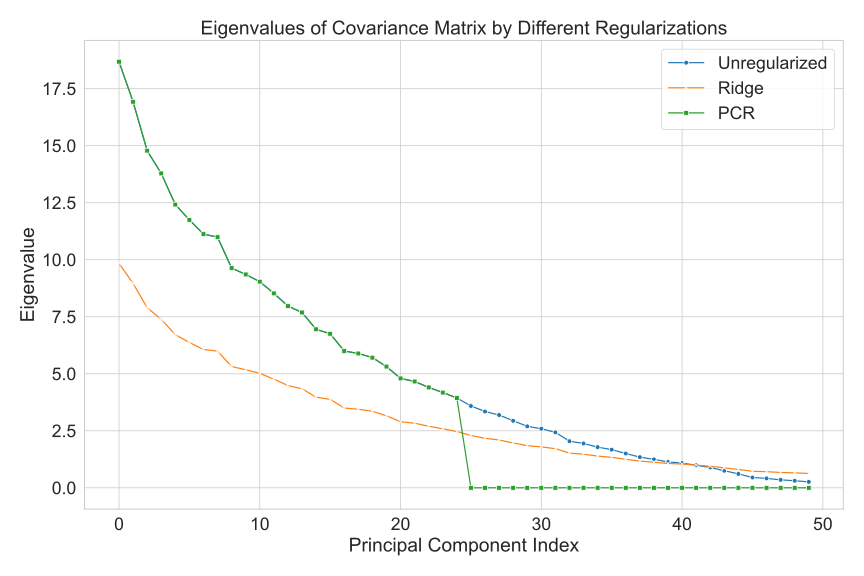
\includegraphics[width=0.9\textwidth]{figures/shrinkage/shrinkage}
    \caption{Comparison of the effect of OLS, Ridge, and PCA regularisation on the eigenvalues of the covariance matrix.}\label{fig:shrinkage}
\end{figure}

When these effective covariance matrices are inverted to form the CCA objective, these effects are reversed.
Ridge regularisation increases the magnitude of the weights associated with the largest eigenvalues and decreases the magnitude of the smallest eigenvalues.
PCA maintains the weights associated with the largest eigenvalues and sets the weights associated with the smallest eigenvalues to zero.
The visualisation underscores the intrinsic nature of each regularisation method:
\begin{itemize}
    \item \textbf{Unregularised}: Presents the unaltered spectrum, making it susceptible to noise but preserving potential subtle patterns.
    \item \textbf{Ridge}: Warps the spectrum, shrinking the largest eigenvalues and expanding the smallest eigenvalues, potentially missing subtle patterns but offering a cleaner representation of stronger associations.
    \item \textbf{PCA}: Truncates the spectrum, ignoring the smallest eigenvalues and preserving the largest eigenvalues, potentially missing subtle patterns but offering a cleaner representation of stronger associations.
\end{itemize}

However, while these shrinkage techniques can improve the performance of CCA, they do not obviously improve the interpretability of the results.
Weights are shrunk towards zero, but they are not set to zero.
This means that the model still uses all the features, and the results are not sparse.

\subsection{Sparse Regularisation}

Sparse regularisation is a powerful tool for improving the performance and interpretability of linear models.
Sparse regularisation encourages the model to use only a subset of the features, which can both help to avoid overfitting and improve the interpretability of the model.
Sparse regularisation works on the premise that only a subset of the features are relevant to the model.
Sparsity is typically achieved by adding either an L1 penalty or constraint\footnote{The L0 norm of the weight vector is the number of non-zero elements in the vector and is arguably a closer match to the goal, but the L0 norm is (a) not a proper norm in the mathematical sense and (b) not convex and so is difficult to optimize.}.
The L1 penalty is defined as:

\begin{align}
    \|u\|_1 = \sum_i |u_i|
\end{align}

Intuitively, this is the sum of the absolute values of the elements of the vector.
Now, with a foundational understanding of sparse regularisation, we review a number of approaches to adding sparsity to the CCA problem.

\paragraph{Sparse PLS: Penalised Matrix Decomposition}
Penalised Matrix Decomposition (PMD)~\citep{witten2009penalized} provides an approximate solution to the sparse CCA problem by altering the constraints of the classical CCA formulation.
Specifically, PMD replaces the constraints \(u\spsT{i} \hat{\Sigma_{ii}} u\sps{i} = 1\) with the PLS constraints \(u\spsT{i} u\sps{i}= 1\) and additionally imposes \(\|u\spsT{i}\|_1 \leq \tau\).
The optimisation problem for PMD is then given by:

\begin{align}
    & u^{opt}=\underset{u}{\mathrm{argmax}}\{ u\spsT{1} \hat{\Sigma_{12}} u\sps{2} \} \\
    & \text{subject to:} \notag \\
    & u\spsT{1} u\sps{1} = 1 , u\spsT{2} u\sps{2} = 1 \notag \\
    & \|u\sps{1}\|_1 \leq \tau_1 , \|u\sps{2}\|_1 \leq \tau_2 \notag
\end{align}

This Sparse PLS (SPLS) approximation has been highly influential as a form of Sparse CCA because it is extremely computationally efficient method \footnote{it can be solved by a variant of the power method; iteratively multiplying $u\sps{1}$ by $\hat{\Sigma_{12}}$ and soft-thresholding}.
Like the relationship between PLS and CCA, PMD and a form of CCA with constrained L1 norm are equivalent only when the covariance matrices are identity matrices.
There are a number of other sparse CCA methods that employ the PLS approximation \citep{parkhomenko2009sparse, waaijenborg2008quantifying, lindenbaum2021l0}.
However, while the PLS approximation is efficient, it means these methods inherit a bias towards the largest principal components from PLS.

To address these problems and truly tackle the sparse CCA optimisation, another class of approaches have adopted a penalised least squares approach.

\paragraph{Sparse CCA: Least Squares Approaches}

It is well known that the CCA problem can be formulated as a constrained least squares problem with the intuition that
for \(X\sps{1} u\sps{1}=1\) and \(X\sps{2} u\sps{2}=1\), correlation is maximised when the squared distance
between \(X\sps{1} u\sps{1}\) and \(X\sps{2} u\sps{2}\) is minimised. \citep{golub1995canonical} proved the
convergence of a simple algorithm which alternates between solving the least squares problem for \(u\sps{1}\) and
\(u\sps{2}\) while keeping the other fixed.

With this intuition, \cite{wilms2015sparse} and \cite{mai2019iterative} separately proposed iterative penalised least
squares methods for sparse CCA\@.

\begin{align}
    \label{eq:mai}
    u^{opt} &= \underset{u}{\mathrm{argmin}} \left\{ \|X\sps{1}u\sps{1} - X\sps{2}u\sps{2}\|_2^2 + P(u) \right\} \\
    &\text{subject to:} \notag \\
    &u\spsT{1} \hat{\Sigma_{11}} u\sps{1}=1 \notag \\
    &u\spsT{2} \hat{\Sigma_{22}} u\sps{2}=1 \notag
\end{align}

Where \(P(u)\) is a penalty function.
The penalty term can be any function that penalises the norm of the vector \(u\).
\citep{mai2019iterative} proved that solving the subproblems where one of $u\sps{i}$ is fixed is easy for one-homogenous $P$ where
\( P((\mu + 1)\theta) = (\mu + 1)P(\theta) \) which notably includes the lasso penalty.
This means a sparse CCA based
on alternating lasso regressions can be solved relatively efficiently using existing solvers.
However, the one homogenous penalty in practice limits the flexibility of the method.
For example, the elastic net penalty is not one-homogenous and therefore cannot be used with this method.
\citet{6556581} and \cite{Mullins2021} added ridge penalties to the subproblems to improve the conditioning of the problem in a way that could be considered a form of elastic net regularisation but the subproblems no longer correctly optimize the global objective\footnote{when rescaling the penalised solutions back to unit variance}.

\paragraph{Sparse CCA: Proximal Gradient Descent and ADMM}
\citet{kanatsoulis2018structured} proposed solving equation~\ref{eq:mai} for more general classes of $P$ using the alternating direction method of multipliers (ADMM)~\citep{boyd2011distributed}.
\cite{fu2017scalable} propose a regularised CCA based on an alternative classical CCA formulation, sometimes called the MAXVAR formulation, which views the problem as a constrained least squares with an auxiliary representation $T$\citep{carroll1968generalization,kettenring1971canonical}.

\begin{align}
    \label{eq:fu}
    \underset{U, T}{\mathrm{argmin}}\left\{\sum_i \|X\sps{i} U\sps{i} - T\|_F^2\right\}\\
    \text{subject to: }T^\top T = I\\
\end{align}

In this formulation, \(U\sps{i}\) represents the \gls{weights} for the $i^{\text{th}}$ view, and \(T\) denotes the latent variable matrix.
The premise is that when \(T\) closely mirrors \(X\sps{i} U\sps{i}\) across all \(i\), the scores correlate.
Notably, this method is adaptable to multiple views.
The authors employed proximal gradient descent for regularisation, specifically suited for penalties like the lasso.
While these methods are flexible, they don't have the plug-and-play nature of the penalised least squares methods.
Not just a matter of convenience, this means that these methods are not compatible with existing solvers for regularised least squares problems like for example total variation regularisation solvers in nilearn, which are often highly optimised for specific problems and modalities.

\paragraph{Structured Regularisation}

As highly structured data, linear models using both structural \acrshort{mri} and f\acrshort{mri} data have been shown to benefit from structured regularisation methods but notably these methods have not been applied to CCA.
Total variation regularisation, which biases spatially neighboring weights to be similar, has been shown to improve the performance of PCA \citep{de2017structured} and regression \citep{michel2011total,dohmatob2014benchmarking, baldassarre2012structured}.
Similarly, Laplacian (or GraphNet) regularisation, which induces a similar spatial bias with additional smoothness, has been shown to improve the performance of CCA on functional MRI data \citep{grosenick2013interpretable,cuingnet2012spatial}.

Having discussed the benefits of both shrinkage (e.g., PCA-CCA, Ridge CCA, PLS), sparsity (SPLS, Sparse CCA), and structure (Total Variation, Laplacian) in handling high-dimensional, noisy, and structured data, a natural progression is to integrate these advantages.
Specifically, the challenge lies in creating a framework that allows for users to match the regularisation method to their data and research question, enhancing the interpretability and performance of Brain-Behaviour association models.
This led us to propose the Flexible Regularised Alternating Least Squares (FRALS).

\section{Methods: Flexible Regularised Alternating Least Squares (FRALS)}\label{subsec:flexible-regularised-alternating-least-squares-(frals)}

The primary goal of our Flexible Regularised Alternating Least Squares framework is to provide a versatile and user-friendly interface for Canonical Correlation Analysis (CCA). This is achieved by designing the framework to be compatible with any scikit-learn compatible regularised least squares solver.
This compatibility is pivotal as it allows researchers and practitioners to leverage the extensive range of solvers available in scikit-learn, a popular machine learning library in Python.

This approach marks a significant departure from traditional methodologies in CCA, which often focused on developing or utilizing specific solvers tailored for particular types of data or computational constraints.
By contrast, \acrshort{frals} democratises access to advanced CCA techniques, allowing users to select solvers that best fit their specific data characteristics, computational needs, or familiarity.
Such flexibility is particularly advantageous in interdisciplinary fields like neuroimaging, where diverse datasets and varying levels of technical expertise are common.

For example, users dealing with high-dimensional, sparse neuroimaging data could opt for solvers optimised for such datasets, while those needing parallel computation for large data sets might choose solvers with GPU acceleration capabilities.
In principle, \acrshort{frals} can even be used with Neural Network-based solvers, which are becoming increasingly popular in machine learning\footnote{Though for reasons that will later become clear, we do not reccommend this!}.
This adaptability enhances \acrshort{frals}' accessibility and future-proofs the framework against evolving computational technologies and data analysis needs.

In the \acrshort{frals} framework, we consider the formulation for a single latent variable \(t\) with regularisation \(\lambda_i P_i\) on the weights \(u^{(i)}\):

\begin{align}
    \underset{u}{\mathrm{argmin}}\left\{\sum_i \|X^{(i)} u^{(i)} - t\|_2^2 + \textcolor{red}{\lambda_i P_i(u^{(i)})} \right\}\\
    \text{subject to: }t^\top t = 1 \notag
\end{align}

This problem can be decomposed into three subproblems.
The first subproblem for the auxiliary variable \(t\):

\begin{align}
    \underset{t}{\mathrm{argmin}}\left\{\sum_i \|X^{(i)} u^{(i)} - t\|_2^2\right\}\\
    \text{subject to: }t^\top t = 1 \notag
\end{align}

is a standard least squares problem and can be solved in closed form by averaging \(X^{(i)} u^{(i)}\) and normalizing i.e. \(t = \frac{\sum_i X^{(i)} u^{(i)}}{\|\sum_i X^{(i)} u^{(i)}\|_2}\).
As shown earlier this makes \(t\) an estimate of the latent variables of a generative CCA model.

The subproblems for the weights \(u^{(i)}\):

\begin{align}
    \underset{u^{(i)}}{\mathrm{argmin}}\left\{\|X^{(i)} u^{(i)} - t\|_2^2 + \textcolor{red}{\lambda_i P_i(u^{(i)})} \right\}
\end{align}

are regularised least squares problems that can be solved using any suitable regularised least squares solver\footnote{We could also in principle replace $X^{(i)} u^{(i)}$ with $f(X^{(i)})$ for any function $f$ including kernels, neural networks, or random forests}.

In this chapter, we illustrate the power of the \acrshort{frals} framework by implementing the well-tested Elastic Net solver from the \texttt{scikit-learn} package~\citep{pedregosa2011scikit}, where \(P_i = \alpha_i \times \text{l1\_ratio} \|u^{(i)}\|_1 + \alpha_i \times (1-\text{l1\_ratio}) \|u^{(i)}\|_2^2\), allowing for independent tuning of shrinkage and sparsity of the weights in both views.

In summary, the \acrshort{frals} framework is a flexible and user-friendly interface for CCA that allows users to combine scikit-learn compatible regularised least squares solvers to solve regularised CCA problems.

\section{Experiment Design}

This section outlines the methodologies used in our study to explore the Flexible Regularized Alternating Least Squares (FRALS) and associated techniques in Canonical Correlation Analysis (CCA). We focus on fitting a single latent dimension for the analyses.

\subsection{Datasets}\label{subsec:datasets}

For this chapter, we chose the \acrshort{hcp} and the \acrshort{adni} datasets to facilitate comparison with two influential brain-behaviour studies \citep{smith2015positive, monteiro2016multiple} as well as the tutorial paper that this chapter is loosely related to \citep{mihalik2022canonical}.
We are particularly interested in the performance of an Elastic Net \acrshort{frals} on these datasets as Ridge CCA has been shown to outperform PLS \citep{mihalik2022canonical}, implying that shrinkage regularisation is beneficial, and Sparse PLS has been shown to outperform PLS \citep{monteiro2016multiple}, implying that sparsity is beneficial. 
We therefore expect that Elastic Net \acrshort{frals} will outperform PLS, Ridge CCA, and Sparse PLS on these datasets.

\subsection{The Predictive Framework for CCA}\label{subsec:the-predictive-framework-for-cca}

Our evaluation of CCA models used a standard predictive framework, dividing the data into an 80:20 ratio for training and testing. This method ensures fitting the model on the training set without incorporating information from the test set.

\subsubsection{Model Comparisons}

The experiment aims to demonstrate the effectiveness of tunable shrinkage and sparsity in CCA models, enabled by the FRALS framework.
We compare the performance of Elastic Net FRALS with other CCA variants such as PCA, PLS, Ridge CCA, SPLS, and Elastic Net CCA, particularly in the context of high-dimensional datasets like HCP and ADNI\@.

\begin{table}[h]
    \centering
    \caption{Employed CCA Variants}
    \begin{tabular}{|l|l|l|l|}
        \hline
        \textbf{Model}               & \textbf{Abbreviation} & \textbf{Hyperparameters}                         & \textbf{Hyperparameter Range} \\
        \hline
        Principal Component Analysis & PCA                   & -                                                & -                             \\
        \hline
        Regularised CCA              & RCCA                  & \(c_1, c_2\)                                     & 0-1 (log scaled)              \\
        \hline
        FRALS - Elastic              & Elastic               & \(\alpha_1, \alpha_2, \text{l1}_1, \text{l1}_2\) & (1e-5,1e-1), (0-1)            \\
        \hline
        Partial Least Squares        & PLS                   & -                                                & -                             \\
        \hline
        Sparse PLS                   & SPLS                  & \(\tau_1, \tau_2\)                               & 0-1 (log scaled)              \\
        \hline
    \end{tabular}\label{tab:cca-variants}
\end{table}

\subsubsection{Model Selection}

For models that require hyperparameter tuning, a grid search was employed to find the best hyperparameters. 
We used 5-fold cross-validation to assess the performance of each model with various hyperparameters across different training data splits. 
The optimization goal was to achieve the highest average out-of-sample correlation.

\subsubsection{The Human Connectome Project (\acrshort{hcp})}

The \acrshort{hcp} offers publicly available resting-state functional MRI (rs-fMRI) and non-imaging measures like demographics, psychometrics, and other behavioral measures.
Specifically, we sourced data from 1003 subjects out of the 1200-subject data release of the \acrshort{hcp}.
The rs-fMRI data provided brain connectivity matrices. These were derived from pairwise partial correlations between subject components obtained through group independent component analysis (ICA), utilizing 25 components. This resulted in 300 brain variables, corresponding to the lower triangle of the connectivity matrix. In our analysis, 145 non-imaging subject measures were incorporated, similar to prior studies, with the exception of 13 measures (ASR\_Aggr\_Pct, ASR\_Attn\_Pct, ASR\_Intr\_Pct, ASR\_Rule\_Pct, ASR\_Soma\_Pct, ASR\_Thot\_Pct, ASR\_Witd\_Pct, DSM\_Adh\_Pct, DSM\_Antis\_Pct, DSM\_Anxi\_Pct, DSM\_Avoid\_Pct, DSM\_Depr\_Pct, DSM\_Somp\_Pct) that were unavailable in the 1200-subject data release. Furthermore, nine confounding variables, including the acquisition reconstruction software version, a summary statistic of head motion during rs-fMRI acquisition, weight, height, systolic and diastolic blood pressure, hemoglobin A1C level, and cube-root of total brain and intracranial volumes as estimated by FreeSurfer, were regressed out from both data types.
More details can be found in \citet{smith2015positive, mihalik2022canonical}.
We summarize the parameters of the \acrshort{hcp} data in table~\ref{tab:hcp-parameters}.

\begin{table}
    \centering
    \caption{HCP Data Parameters}
    \begin{tabular}{| l | l |}
        \hline
        \textbf{Parameter}                        & \textbf{Value} \\
        \hline
        Number of samples (\textit{n})            & 1003           \\
        Number of features in View 1 (\textit{p}) & 300          \\
        Number of features in View 2 (\textit{q}) & 145            \\
        \hline
    \end{tabular}\label{tab:hcp-parameters}
\end{table}

\subsubsection{The Alzheimer's Disease Neuroimaging Initiative (ADNI)}

Accessible at \url{adni.loni.usc.edu}, the \acrshort{adni} database was initiated in 2003. 
Its primary aim is the examination of how well serial MRI, PET (Positron Emission Tomography), biological markers, along with clinical and neuropsychological assessments, track the progression of Mild Cognitive Impairment (MCI) and the early stages of Alzheimer’s disease. 
In our study, we utilised data from a subset of 592 unique individuals, comprising 309 males (average age 74.68 ± 7.36 SEM) and 283 females (average age 72.18 ± 7.50 SEM). This subset included 147 healthy controls, 335 individuals with Mild Cognitive Impairment (MCI), and 110 diagnosed with dementia. 
T1 weighted structural MRI (sMRI) scans were the source of whole-brain voxel-based grey matter volumes. The sMRI data underwent preprocessing with SPM12 \citep{ashburner2014spm12}, which involved segmentation, normalisation using DARTEL, reslicing to a resolution of \(2 \times 2 \times 2 \, \text{mm}^3\)
, and spatial smoothing using a Gaussian kernel with 2 mm full width at half maximum (FWHM). A grey matter voxel selection mask, with a threshold of $\geq$10\%, was applied to all participants' scans, resulting in 168,130 brain variables. 
The Mini-Mental State Examination (MMSE) is a widely recognised neurocognitive test comprising 30 questions across five cognitive domains\citep{folstein1975mini}: orientation (questions 1-10), registration (questions 11-13), attention and calculation (questions 14-18), recall (questions 19-21), and language (questions 22-30).
An additional item was included in our study to account for the number of attempts a subject needed to correctly respond to the registration domain questions, leading to a total of 31 variables. As in \citet{monteiro2016multiple}, no confounds were removed from these data.
We summarize the parameters of the \acrshort{adni} data in table~\ref{tab:adni-parameters}.

\begin{table}
    \centering
    \caption{ADNI Data Parameters}
    \begin{tabular}{| l | l |}
        \hline
        \textbf{Parameter}                        & \textbf{Value} \\
        \hline
        Number of samples (\textit{n})            & 592            \\
        Number of features in View 1 (\textit{p}) & 168130         \\
        Number of features in View 2 (\textit{q}) & 31             \\
        \hline
    \end{tabular}\label{tab:adni-parameters}
\end{table}

\subsection{The predictive framework for CCA}\label{subsec:the-predictive-framework-for-cca}

To evaluate the performance of CCA models, we employ a standard predictive framework.
We split the data into training and test sets using a 80:20 split, and use the training set to fit the model.
We then use the test set to evaluate the model's performance.
Where relevant, pre-processing is performed on the training set and the same pre-processing is applied to the test set.
This is important to avoid data leakage, where information from the test set is used to fit the model.

\subsubsection{Model Comparisons}
In the experiments in this section, we are interested in illustrating the effects of tunable shrinkage and sparsity on the performance and interpretability of CCA models, enabled by the \acrshort{frals} framework.
To this end, we compare the performance of Elastic Net \acrshort{frals} with other CCA variants, including PCA, PLS, Ridge CCA, Sparse PLS, and Elastic Net CCA\@.
Since the \acrshort{hcp} and \acrshort{adni} data are high-dimensional, we drop CCA from the analysis since it would produce random results.

\begin{table}[h]
    \centering
    \caption{Employed CCA Variants}
    \begin{tabular}{|l|l|l|l|}
        \hline
        \textbf{Model}               & \textbf{Abbreviation} & \textbf{Hyperparameters}                         & \textbf{Hyperparameter Range}                                                                                             \\
        \hline
        Principal Component Analysis & PCA                   & -                                                & -                                                                                                                         \\
        \hline
        Regularised CCA              & RCCA                  & \(c_1, c_2\)                                     & 0-1 (log scaled)                                                                                                          \\
        \hline
        FRALS - Elastic              & Elastic               & \(\alpha_1, \alpha_2, \text{l1}_1, \text{l1}_2\) & (1e-5,1e-1), (0-1)                                                                                                        \\
        \hline
        Partial Least Squares        & PLS                   & -                                                & -                                                                                                                         \\
        \hline
        Sparse PLS                   & SPLS                  & \(\tau_1, \tau_2\)                               & 0-1\footnote{As in \citet{witten2013package}, these are converted to 0-$\sqrt {\text{number of features}}$)} (log scaled) \\
        \hline
    \end{tabular}\label{tab:cca-variants}
\end{table}

\subsubsection{Model Selection}

For the models that require hyperparameter tuning, we use a grid search to find the best hyperparameters.
Specifically, we use 5-fold cross-validation to evaluate the performance of a model with a given set of hyperparameters on 5 different splits of the training data with non-overlapping validation sets.
We optimise for the hyperparameters that give the best average out of sample correlation.

\section{Experiment Results}

\subsection{\acrshort{hcp} Results}

Next, we consider the results of applying the various CCA variants to the \acrshort{hcp} data.

\subsubsection{Out of Sample Correlation}

Both Ridge CCA and Elastic Net outperformed PLS and SPLS in terms of holdout correlation captured (Figure~\ref{fig:performance}).
This suggests that tunable L2 regularisation is important, even for very high-dimensional data, and that resorting to PLS is suboptimal.
On the other hand, while the additional sparsity improved SPLS over PLS (consistent with previous work \cite{monteiro2016multiple}), it did not improve the performance of the Elastic Net model over Ridge CCA\@.

\begin{figure}[h]
    \centering
    \includegraphics[width=0.5\linewidth]{figures/hcp/holdout_correlations}
    \caption{\textbf{HCP:} Comparative out-of-sample canonical correlations among PCA, RCCA, ElasticNet, PLS, and SPLS models. The bars represent the correlation coefficients, indicating that Ridge CCA and Elastic Net models have superior performance over PLS and SPLS in capturing holdout correlation.}
    \label{fig:performance}
\end{figure}

Nonetheless, the Elastic Net model demonstrated a more sparse representation than the Ridge CCA model, with the Elastic Net model utilizing 241 and 96 non-zero weights for the brain and behaviour views, respectively (Table~\ref{tab:sparse-weights-hcp}). In contrast, the Ridge CCA model used 300 and 145 non-zero weights for the respective views.
Moreover, the SPLS model achieved an even sparser solution with only 118 and 56 non-zero weights for the brain and behaviour views. Considering the comparable performance of the Elastic Net and Ridge CCA models, the former's sparsity may offer a preferable solution.

\begin{table}[h]
    \centering
    \caption{\textbf{HCP:} Sparsity of models reflected by the count of non-zero weights. Elastic Net and SPLS demonstrate increased sparsity in the model weights for both brain and behaviour views, compared to PCA, RCCA, and PLS.}
    \begin{tabular}{|c|c|c|}
        \hline
        Model       & Brain Weights (out of 300) & Behaviour Weights (out of 145) \\
        \hline
        PCA         & 300           & 145               \\
        RCCA        & 300           & 145               \\
        Elastic Net & 241           & 96                \\
        PLS         & 300           & 145               \\
        SPLS        & 118           & 56                \\
        \hline
    \end{tabular}\label{tab:sparse-weights-hcp}
\end{table}

\subsubsection{Behaviour Weights}

Figure~\ref{fig:behaviour} presents the top eight positive and negative non-imaging weights for each model to visualize the behavioural data variations observed in the previous section. The PCA model emphasizes a mode of variation with positive correlations to psychiatric and life function tests, contrasting with negative correlations to certain emotion and personality tests. In comparison, the RCCA and Elastic Net models highlight a variation mode negatively correlated with the Line Orientation test and to a lesser extent, smoking, while showing positive correlations with other cognitive assessments. The PLS model's variation mode echoes the positive-negative pattern identified by \cite{smith2015positive}, showing positive correlations with agreeableness, vocabulary tests, and life satisfaction, juxtaposed with strong negative correlations with smoking and antisocial behaviors. SPLS selects a similar mode but prioritizes vocabulary tests and smoking over rule-breaking and antisocial personality traits, aligning with the preprocessing steps described in \cite{smith2015positive} which incorporated a top-100 PCA projection of both brain and behavioural data.

\begin{figure}[h]
    \centering
    \includegraphics[width=0.8\linewidth]{figures/hcp/PCA behaviour weights}
    \includegraphics[width=0.8\linewidth]{figures/hcp/RCCA behaviour weights}
    \includegraphics[width=0.8\linewidth]{figures/hcp/ElasticNet behaviour weights}
    \includegraphics[width=0.8\linewidth]{figures/hcp/PLS behaviour weights}
    \includegraphics[width=0.8\linewidth]{figures/hcp/SPLS behaviour weights}
    \caption{\textbf{HCP:} Behavioural weights highlighting the top-8 positive and negative non-imaging weights. Each subfigure represents a distinct model's weight distribution across various behavioural domains such as cognition, emotion, personality, substance use, alertness, and psychiatric and life function. The variations in the weight profiles across models reflect differing patterns of association with the behavioural traits considered in the study.}
\end{figure}

\subsubsection{Brain Connectivity Weights}

In this section, we use two different methods to visualize the brain connectivity weights.
The first method is to use chord diagrams to visualize the top 8 positive and negative brain \gls{weights} for each model.
This approach is inspired by the chord diagrams used in \cite{smith2015positive}.
The second method is to use surface maps to visualize the brain connectivity weights.
This approach has been used by both \cite{ferreira2022hierarchical} and \cite{smith2015positive}.

\paragraph{Chord Diagrams}
We grouped the nodes of the connectivity matrix of our data into 7 parcels according to the Yeo 7 network parcellation \cite{yeo2011organization}.
This was achieved by assigning each node to the network with the highest voxelwise overlap.
These are then arranged around the circumference of the chord diagram using the Nichord package \citep{bogdan2023connsearch}.
The plots then show the 8 strongest positive and negative \gls{weights} for each model as `chords'.
The chord diagrams in Figure~\ref{fig:chord_weights} show the top 8 positive and negative brain \gls{weights} for each model.

\begin{itemize}
    \item The \textbf{RCCA} model displays a diverse set of connections across all networks, with especially prominent weights in the \textcolor{red}{somatomotor} and \textcolor{blue}{default mode} networks.

    \item The \textbf{ElasticNet} model presents similar connections between the \textcolor{red}{somatomotor} and \textcolor{blue}{default mode} networks.

    \item The \textbf{PLS} model exhibits strong connections between the \textcolor{green}{frontoparietal} and \textcolor{pink}{visual} networks.

    \item The \textbf{SPLS} model exhibits similar connections between the \textcolor{green}{frontoparietal} and \textcolor{pink}{visual} networks.
\end{itemize}

This is perhaps consistent with the behaviour data as the somatomotor network is associated with motor function and sensory processing which is related to the Line Orientation test, requiring spatial reasoning and motor coordination.

The correlations made by the PLS and SPLS models between substance abuse and cognitive tests could be due to the significant role the frontoparietal network plays in executive function, which can be impaired by substance abuse.
Likewise, the visual network is likely involved in a number of the cognitive tests and could be disrupted by substance abuse.

The RCCA and ElasticNet models might be detecting more integrative and possibly higher cognitive functions, while the PLS and SPLS models might be highlighting the more immediate cognitive processes that can be disrupted by substance abuse.

\begin{figure}[h]
    \centering
    \includegraphics[width=0.49\linewidth]{figures/hcp/RCCA brain weights}
    \includegraphics[width=0.49\linewidth]{figures/hcp/ElasticNet brain weights}
    \includegraphics[width=0.49\linewidth]{figures/hcp/PLS brain weights}
    \includegraphics[width=0.49\linewidth]{figures/hcp/SPLS brain weights}
    \includegraphics[width=0.49\linewidth]{figures/hcp/PCA brain weights}
    \caption{\textbf{HCP:} Brain connectivity weights visualized through chord diagrams for multiple models. Each diagram portrays the 8 strongest positive (red to blue gradient) and negative (blue to red gradient) weights, grouped by the Yeo 7 network parcellation.}\label{fig:chord_weights}
\end{figure}

\subsubsection{Model Similarity}

In this section, we compare the models in terms of their similarity.
We can measure the pairwise similarity between two models by comparing their \gls{weights} and their \gls{representations}.
We can compare the \gls{weights} by computing the correlation between the \gls{weights} of the two models and we can compare the \gls{representations} by computing the correlation between the \gls{representations} of the two models.

In Figure~\ref{fig:brain-behaviour-scores-sim}, we plot the correlation between the brain and behaviour \gls{representations} for each model. 
We can see clearly that both PCA, PLS, and SPLS are all highly correlated in terms of their brain representations, revealing the bias of PLS towards the largest principal components.
On the other hand, in the behaviour space, the models are less correlated, with the exception of PLS and SPLS which are highly correlated with one another. 
There is however still substantial correlation between the PCA and PLS models.
The very low correlation between the Ridge CCA and Elastic Net models with the PCA model is evidence that there are stronger correlations outside of the first principal components.

In Figure~\ref{fig:brain-behaviour-weights-sim}, we similarly plot the correlation between the brain and behaviour \gls{weights} for each model. 
The story is similar, albeit with marginally lower correlations between the PLS and PCA-based models. Finally, in the weights space, the Ridge CCA and ElasticNet models are even less correlated with the PCA model.

\begin{figure}
    \centering
    \includegraphics[width=0.8\linewidth]{figures/hcp/brain and behaviour scores correlation}
    \caption{\textbf{HCP:} Pairwise correlation matrix of brain representations across different models. The high correlation coefficients between PCA, PLS, and SPLS indicate a significant overlap in the brain representations they produce, suggesting a bias of PLS toward principal components. Contrarily, the Ridge CCA and Elastic Net models show notably lower correlations with PCA, indicating that these models capture brain representations beyond the first principal components.}\label{fig:brain-behaviour-scores-sim}
\end{figure}

\begin{figure}
    \centering
    \includegraphics[width=0.8\linewidth]{figures/hcp/brain and behaviour weights correlation}
    \caption{\textbf{HCP:} Pairwise correlation matrix of the brain and behaviour weights used by each model. Similar to the brain representations, PCA, PLS, and SPLS show a high correlation in their weights, indicating similarity in the factors they consider significant. The lower correlations observed for Ridge CCA and Elastic Net with PCA suggest that these models give importance to different aspects of the data, potentially capturing more nuanced relationships.}\label{fig:brain-behaviour-weights-sim}
\end{figure}


\subsection{\acrshort{adni} Results}\label{subsec:adni}


\subsubsection{Out of Sample Correlation}

In this experiment, the Elastic Net model outperformed all other models in terms of out-of-sample correlation (Figure~\ref{fig:adni-performance}).
The RCCA model also outperformed the PLS and SPLS models while SPLS outperformed PLS.
Suprisingly, PCA performed almost as well as PLS.
This suggests that there is value in both tunable shrinkage and sparsity in this dataset.
It also reveals that the correlated signal between the brain structure and behavioural data is relatively much stronger than in the \acrshort{hcp} data.

\begin{figure}
    \centering
    \includegraphics[width=0.5\linewidth]{figures/adni/holdout_correlations}
    \caption{\textbf{ADNI:} Comparative out-of-sample canonical correlations among PCA, RCCA, ElasticNet, PLS, and SPLS models. The bars represent the correlation coefficients, indicating that the Elastic Net models has superior performance over Ridge CCA, PLS, and SPLS in capturing holdout correlation.}\label{fig:adni-performance}
\end{figure}

\subsubsection{Sparsity of Weights}

Table~\ref{tab:brain-behaviour-weights-adni} once again shows the number of non-zero \gls{weights} for each model.
We can see that tuned SPLS and Elastic Net once again identify sparse weights.
In this case, the difference in performance is more convincing and suggests that this sparsity is less spuriously induced than for the \acrshort{hcp} data.
This is supported by the fact that Elastic Net and SPLS models find a similar level of sparsity in the brain weights.
On the other hand SPLS finds a much sparser set of behavioural weights.

\begin{table}
    \centering
    \caption{\textbf{ADNI:} Number of non-zero \gls{weights} for each model.}
    \begin{tabular}{|c|c|c|}
        \hline
        Model       & Brain Weights (out of 168130) & Behaviour Weights (out of 31) \\
        \hline
        PCA         & 168130        & 31                \\
        RCCA        & 168130        & 31                \\
        Elastic Net & 59617         & 17                \\
        PLS         & 168130        & 31                \\
        SPLS        & 74995         & 10                \\
        \hline
    \end{tabular}\label{tab:brain-behaviour-weights-adni}
\end{table}

\subsubsection{Behaviour Weights}

As for the \acrshort{hcp} data, Figure \ref{fig:adni-beh} plots the top 8 positive and negative non-imaging \gls{weights} for each model.
Some of the identified behavioural \gls{weights} including a number of orientation tests are similar across all of the models, including even PCA.
This is indicative of the strong shared signal between the behavioural data and the brain structure data.
SPLS and Elastic Net both emphasize the orientation and recall tests in the weight space.
The RCCA and Elastic Net models are suprisingly different in the weight space, with the RCCA \gls{weights} on a couple of attention and calculation tests in addition to the ubiquitous orientation and recall tests.

\begin{figure}
    \centering
    \includegraphics[width=0.8\linewidth]{figures/adni/PCA behaviour weights}
    \includegraphics[width=0.8\linewidth]{figures/adni/RCCA behaviour weights}
    \includegraphics[width=0.8\linewidth]{figures/adni/ElasticNet behaviour weights}
    \includegraphics[width=0.8\linewidth]{figures/adni/PLS behaviour weights}
    \includegraphics[width=0.8\linewidth]{figures/adni/SPLS behaviour weights}
    \caption{\textbf{ADNI:} Bar plots of the behaviour \gls{weights} for each model.}\label{fig:adni-beh}
\end{figure}

\subsubsection{Brain Structure Weights}

We plot the \gls{weights} as a mosaic plot with 3 slices in each direction in Figure~\ref{fig:adni-brain}.
Previous work using SPLS with the \acrshort{adni} dataset identified the same striking pattern of \gls{weights} with the model strikingly selecting the hippocampal weights \citep{monteiro2016multiple}.
The Elastic Net has a less visually appealing selection of weights, with a honeycomb pattern near the edges of the brain and likewise for RCCA.
It is noticeable that PCA, PLS and SPLS both \gls{weights} in the same direction whereas RCCA and Elastic Net weight different regions with opposite signs.

\begin{figure}
    \centering
    \includegraphics[width=0.45\linewidth]{figures/adni/PCA brain weights mosaic}
    \includegraphics[width=0.45\linewidth]{figures/adni/RCCA brain weights mosaic}
    \includegraphics[width=0.45\linewidth]{figures/adni/ElasticNet brain weights mosaic}
    \includegraphics[width=0.45\linewidth]{figures/adni/PLS brain weights mosaic}
    \includegraphics[width=0.45\linewidth]{figures/adni/SPLS brain weights mosaic}
    \caption{\textbf{ADNI:} Statistical maps of brain structure weights for each model.}
\end{figure}

\subsubsection{Model Similarity}

In this section, we once again compare the models in terms of their similarity.
In Figure~\ref{fig:brain-behaviour-scores-sim-adni}, we can see that all of the models are highly correlated in terms of their behaviour \gls{representations}.
The brain \gls{representations} are less correlated, but once again PCA, PLS, and SPLS are highly correlated with one another and less correlated with the Ridge CCA and Elastic Net models.

Suprisingly, in Figure~\ref{fig:brain-behaviour-weights-sim-adni}, we can see that the weights in both views are less correlated.
This is particularly true for the brain \gls{weights} where PCA exhibits a very low correlation with Ridge CCA and Elastic Net.

\begin{figure}
    \centering
    \includegraphics[width=0.8\linewidth]{figures/adni/brain and behaviour scores correlation}
    \caption{\textbf{ADNI:} Correlation between the brain and behaviour \gls{representations} for each model.}\label{fig:brain-behaviour-scores-sim-adni}
\end{figure}

\begin{figure}
    \centering
    \includegraphics[width=0.8\linewidth]{figures/adni/brain and behaviour weights correlation}
    \caption{\textbf{ADNI:} Correlation between the brain and behaviour \gls{weights} for each model.}\label{fig:brain-behaviour-weights-sim-adni}
\end{figure}

\section{Discussion and Limitations}


The Flexible Regularised Alternating Least Squares (FRALS) framework for CCA, introduced in this chapter, exhibits promising performance in terms of out-of-sample correlation.
Our findings indicate that, while Elastic Net CCA generally outperforms other CCA variants, much of the benefit is derived from using properly tuned Ridge regularization.
This is most obviously illustrated in the \acrshort{hcp} dataset where sparsity does not appear to be beneficial in terms of out-of-sample correlation and therefore casts doubt on whether the sparsity of the model is interpretable or spurious.
It also questions whether the additional computational cost of Elastic Net CCA is justified.
Our experiments reveal that Ridge CCA typically outperforms PLS across both datasets.
This observation is akin to the dynamics of regularized regression, where maximal ridge regularization is seldom necessary, even in high-dimensional contexts.

\subsection{FRALS Limitations}

The Flexible Regularised Alternating Least Squares (FRALS) framework, while effective in certain aspects, is notably limited by its computational inefficiency. This inefficiency arises from two main factors: the dynamic nature of regression targets and the intensive computation required for each iteration.

\subsubsection{Changing Regression Targets}

In FRALS, regression targets are not static but dynamically evolve during the algorithm's execution. These targets are essentially projections of the other view, and as they change, they alter the optimization landscape. Consequently, the algorithm must frequently recompute the least squares solution for each view. This process results in significant computational overhead and often leads to redundant calculations, thereby contributing to the inefficiency of the FRALS framework.

\subsubsection{Computational Time}

The primary computational challenge in FRALS is the repeated calculation of the least squares solution for each view in every iteration. This requirement is resource-intensive and is the main factor contributing to the slow speed of the FRALS algorithm. Empirical observations from our experiments show that FRALS operates at a pace approximately 10 times slower than Ridge CCA, varying with the specifics of the experimental setup. This disparity in speed is particularly noteworthy given the popularity of SPLS due to its speed and convenience. Figure \ref{fig:timings} provides an estimate of the time taken to fit each model across complete training datasets over ten runs. It is evident from the figure that Elastic Net CCA, despite being an iterative algorithm, is significantly slower than other models, particularly with the high-dimensional \acrshort{adni} data. While SPLS demonstrates much faster processing, it is only marginally slower than PLS and RCCA, both of which employ optimized solvers in C and use PCA preprocessing for efficiency. Consequently, PCA emerges as the fastest model in these comparisons.

\begin{figure}
    \centering
    \includegraphics[width=0.8\linewidth]{figures/model_fit_timings}
    \caption{Time taken to fit each model over ten runs. The interquartile range is plotted as a box with whiskers drawn to the farthest datapoint within 1.5 times the interquartile range.}\label{fig:timings}
\end{figure}

\subsection{Conclusion}

In this chapter, we introduced the Flexible Regularised Alternating Least Squares (FRALS) framework for CCA\@.
We used the FRALS framework to implement Elastic Net CCA\@.
We then compared the performance of Elastic Net CCA with other CCA variants on two datasets: the \acrshort{hcp} and \acrshort{adni}.
We found that Elastic Net CCA outperformed other CCA variants on both datasets but that the performance of Elastic Net CCA was similar to Ridge CCA on the \acrshort{hcp} dataset.
However, we found that Elastic Net CCA was much slower than other CCA variants.


 \graphicspath{{chapters/loadings/}}


\chapter{Insights From Generating Simulated Data for CCA}\label{ch:loadings}
% \epigraph{All models are wrong, some are useful.}{\textit{G. Box}}
\minitoc
% chktex-file 44
% chktex-file 3
\section*{Preface}

This chapter, deriving insights from various projects, lays out both my arguments for the use of loadings in the interpretation of CCA models and a number of computational tricks that we used to generate simulated data with significantly higher dimensions than have been previously considered in the literature.
The simulated data generation methods were used to generate simulated data in \citet{mihalik2022canonical}.
The arguments for the use of loadings influenced our choice of loadings for the interpretation of the results in \citet{ADAMS2024}.

\section{Introduction}

Despite its popularity, there is an ongoing debate in the CCA literature regarding the interpretation of model weights versus loadings \citep{gu2018simultaneous}. This chapter aims to contribute to this debate by providing mathematical insights from generative models of CCA and empirical results from simulated data with higher dimensionality than previously considered in the literature.

We begin by categorizing methods for generating CCA simulated data into explicit and implicit latent variable models. This categorization allows us to compare and contrast the generative models in CCA literature with the generative model for linear regression. We highlight that in linear regression, regularization can be interpreted as a prior on the weights, whereas in CCA, it is perhaps more natural to interpret regularization as a prior on the loadings. By leveraging computational tricks, we demonstrate how to generate simulated data with significantly higher dimensions than previously considered in the literature \citep{helmer2020stability, matkovivc2023static}.

Furthermore, we rigorously prove that loadings are invariant to columnwise transformations in data matrices, unlike weights. This property makes CCA unique compared to Principal Component Analysis (PCA) or Partial Least Squares (PLS) and is particularly relevant in fields like brain-behavior studies, where data preprocessing often involves columnwise manipulation.

Our experimental design focuses on two main aspects. First, we evaluate the ability of CCA models to accurately recover the true model weights and loadings. Second, we examine the out-of-sample performance, which is often observed to be poor in practical datasets despite statistical significance, particularly for PLS-based models. This observation led us to question whether the issue lies in poor model fit or a lack of signal in the data with weak or biologically spurious correlations.

One of our most striking findings, consistent with the previous chapter, is the efficacy of Ridge Regularized CCA models compared to PLS models in identifying high correlations under anisotropic noise conditions; where the noise covariance matrices ($\Psi$) are not scalar multiples of the identity matrix, leading to non-spherical noise distributions. This complements earlier work \citep{helmer2020stability} that found that the number of samples needed to find high correlations increases with dimensionality; our results suggest that the important variable is the dimensionality of the smaller view.

Through this chapter, we aim to provide a comprehensive understanding of the relationship between weights and loadings in CCA models, the impact of regularization on model interpretation, and the performance of CCA models in high-dimensional settings. By unifying generative perspectives, proving mathematical properties, and conducting extensive simulations, we contribute to the ongoing debate in the CCA literature and provide valuable insights for researchers and practitioners applying CCA in various domains.

\section{Background: Weights and Loadings in Canonical Correlation Analysis}

CCA can be interpreted in two ways: either as a method that finds linear combinations of variables in two datasets that exhibit the highest correlation, or as a technique that estimates latent variables that are maximally correlated.

The concept of latent variables is particularly important in biomedical applications, as it can help uncover underlying factors influencing observable data. For example, in brain-behavior studies, latent variables may represent hidden neurological or cognitive processes that drive the relationship between brain structure or function and behavioral outcomes. Similarly, in imaging-genetics, latent variables can capture the genetic factors that influence brain morphology or activity patterns. By introducing latent variables, CCA enables researchers to gain a deeper understanding of complex phenomena like gene expression, pathologies, and normative variations in health-related data \citep{lawry2023multi}.

\subsection{Generative and Discriminative Approaches in CCA}

CCA's practical application revolves around two main approaches: the discriminative approach and the generative approach. 
The generative approach, known as the `forward model', emphasizes the data generation process and employs loadings to describe the relationship between latent variables and observed data. It models the joint distribution of the observed data conditioned on the latent variables, expressed as $P(X\sps{1},X\sps{2}|Z)$. In this approach, the latent variables are assumed to be the underlying cause\footnote{Used here very loosely to give intuition} of the observed data, and the goal is to learn the parameters of the generative model that best explains the data.

In contrast, the discriminative approach, represented as the `backward model' in Figure~\ref{fig:forward-backward-models}, uses weights to estimate highly correlated latent variables from observed data. It focuses on modeling the conditional distribution of the latent variables given the observed data, denoted as $P(Z|X\sps{1},X\sps{2})$. The discriminative approach aims to find the optimal linear combinations of the observed variables that maximize the correlation between the latent variables, without explicitly modeling the data generation process.

\begin{figure}
    \centering
    \tikz{
    % nodes
        \node[latent, align=center, minimum size=2cm] (Z) {Severity\\z};
        \node[obs, below left=of Z, minimum size=2cm, align=center] (x1) {Brain\\$x^{(1)}$};
        \node[obs, below right=of Z, minimum size=2cm, align=center] (x2) {Behaviour\\$x^{(2)}$};
        % edges
        \edge[blue]{Z} {x1};
        \edge[blue]{Z} {x2};
        \edge[red, tension=0.1]{x1} {Z};
        \edge[red, tension=0.1]{x2} {Z};
    }
    \caption[Forward and Backward Multiview Models]{\textit{\textbf{Forward and Backward Multiview Models:}} The \textcolor{blue}{generative/forward} and \textcolor{red}{discriminative/backward} approaches in \acrshort{cca}.}\label{fig:forward-backward-models}
\end{figure}

\subsection{Analogy Between CCA and PCA}

The distinction between the generative and discriminative approaches in CCA is analogous to the different interpretations of Principal Component Analysis (PCA) \citep{park2023critical}. PCA can also be viewed from a generative perspective, where the observed data are assumed to be generated from latent variables \citep{tipping1999probabilistic}, or from a discriminative perspective, where the principal components are linear combinations of the observed variables that maximize the variance \citep{hotelling1933analysis}.

In both CCA and PCA, the generative approach focuses on modeling the joint distribution of the observed data and the latent variables, while the discriminative approach emphasizes finding the optimal linear combinations of the observed variables to estimate the latent variables or principal components.

\subsection{The Debate Regarding Weights and Loadings in CCA}

In CCA research, there is an ongoing debate regarding the interpretation of models in terms of weights or loadings \citep{gu2018simultaneous}. Weights are often preferred for prediction tasks, as they directly relate the observed variables to the latent variables. On the other hand, loadings are favored for interpretation, as they provide insights into the structure and relationships within the data \citep{liu2022improved}. This discussion is particularly relevant to our work in chapter \ref{ch:als} and various studies involving sparse CCA and sparse Partial Least Squares (PLS), where understanding the meaning and implications of sparse loadings and weights is crucial.

Given the importance of this topic, especially in the context of our work in chapter \ref{ch:als} and other studies employing variants of sparse CCA and sparse PLS, it is essential to delve deeper into the interpretation of sparse loadings and weights. In the following sections, we will explore the mathematical properties and practical implications of weights and loadings in CCA, with a focus on sparse and regularized models. By addressing this key aspect of CCA, we aim to contribute to the ongoing debate and provide insights that can guide the application and interpretation of CCA in various domains, including neuroimaging, genetics, and health-related research.

\section{Methods: Unifying Generative Perspectives in CCA: Explicit and Implicit Latent Variable Models of Multiview Data}

This section categorizes the generative models in CCA literature into explicit and implicit latent variable types, each offering distinct insights into the data generation process and the relationship between weights and loadings.

\subsection{Additional Notational Conventions}

We will use some additional notational convention to describe probabilistic models.
We will use lowercase letters to represent samples from a distribution, and uppercase letters to represent random variables.
For example, \(x\) represents a sample from the distribution \(P(X)\), and \(X\) represents the random variable \(X\).
We will use $\sim$ to denote the sampling process, and $|$ to denote conditioning.
For example, \(x | z \sim \mathcal{N}(\mu, \Psi)\) represents a sample \(x\) from a Gaussian distribution with mean \(Wz\) and covariance \(\Psi\) conditioned on the latent variable \(z\).
We also introduce the notation \(w\sps{i}_{j}\) to refer to the loading of the \(j\)-th feature in the \(i\)-th view on a latent variable, as well as \(W\sps{i}\) to refer to the matrix of loadings for the \(i\)-th view on all latent variables.

\subsection{Explicit Latent Variable Models: Probabilistic CCA and Group Factor Analysis}

Explicit latent variable models assume that the observed data in each view is generated from a shared latent space, with view-specific linear transformations and added noise. These models provide a probabilistic framework for understanding the relationship between multiple views of data and the underlying latent factors that give rise to them.

\subsubsection{Probabilistic CCA}
Probabilistic CCA (PCCA) is an explicit latent variable model that extends classical CCA to a probabilistic setting. In PCCA, the generative process for two views can be described as follows:
\begin{align}
z &\sim \mathcal{N}(0, I)\\
x\sps{i} &\sim \mathcal{N}(W\sps{i} z + \mu\sps{i}, \Psi\sps{i})
\end{align}
where $z$ is a shared latent variable drawn from a standard normal distribution, $x\sps{i}$ represents a sample from the $i$-th view, $W\sps{i}$ are the view-specific loadings that map the latent space to the observed space, $\mu\sps{i}$ is the mean of the $i$-th view, and $\Psi\sps{i}$ is the view-specific noise covariance matrix.

The key idea behind PCCA is that the shared latent variable $z$ captures the common structure across views, while the view-specific loadings $W\sps{i}$ allow for flexibility in how this structure is expressed in each view. The noise covariance matrices $\Psi\sps{i}$ account for view-specific variation not explained by the shared structure.
\citet{bach2005probabilistic} showed that the maximum likelihood estimates of the loadings $W\sps{i}$ in PCCA are related to the classical CCA weights $U\sps{i}$ by the within-view covariance matrices $\Sigma_{ii}$:
\begin{align}\label{eq:weights-to-loadings}
W\sps{i} &= \Sigma_{ii} U\sps{i} R\\
U\sps{i} R &= \Sigma_{ii}^{-1} W\sps{i}
\end{align}
where $R$ is an arbitrary rotation matrix. This result provides a link between the probabilistic and non-probabilistic formulations of CCA, and suggests that the classical CCA weights can be interpreted as estimates of the true loadings, up to a rotation.
\subsubsection{Group Factor Analysis}
Group Factor Analysis (GFA) \citep{klami2014group} is another explicit latent variable model that extends PCCA by assuming isotropic (i.e., spherical) noise in each view:
\begin{align}
z &\sim \mathcal{N}(0, I)\
x\sps{i} &\sim \mathcal{N}(W\sps{i} z + \mu\sps{i}, \sigma_i^2 I)
\end{align}
where $\sigma_i^2$ is the noise variance in the $i$-th view. This assumption simplifies the model and can lead to computational benefits, as well as supporting extensions like sparsity on the loadings.
The joint distribution of multiple views under the GFA model is a multivariate Gaussian distribution with a structured covariance matrix:
\begin{align}
\begin{bmatrix}
X\sps{1} \ \vdots \ X\sps{m}
\end{bmatrix} \sim \mathcal{N} \left( \begin{bmatrix}
\mu\sps{1} \ \vdots \ \mu\sps{m}
\end{bmatrix}, \begin{bmatrix}
W\sps{1}W\spsT{1} + \sigma_1^2 I & \cdots & W\sps{1}W\spsT{m} \\
\vdots & \ddots & \vdots \\
W\sps{m}W\spsT{1} & \cdots & W\sps{m}W\spsT{m} + \sigma_m^2 I
\end{bmatrix} \right)
\end{align}
This highlights the fact that the covariance structure in each view is determined by the view-specific loadings and noise variances. When the loadings $W\sps{i}$ have large singular values compared to the noise variances $\sigma_i^2$, the resulting covariance matrices $\Sigma_{ii} = W\sps{i}W\spsT{i} + \sigma_i^2 I$ are often referred to as "spiked covariance matrices" \citep{johnstone2001distribution}.

\subsubsection{Connecting GFA and Probabilistic PCA}
Probabilistic PCA (PPCA) \citep{tipping1999probabilistic} is a special case of GFA applied to a single view:
\begin{align}
z &\sim \mathcal{N}(0, I)\\
x &\sim \mathcal{N}(W z + \mu, \sigma^2 I)
\end{align}
Like GFA, PPCA assumes isotropic noise and seeks to identify a lower-dimensional latent space that captures the structure in the observed data. The key difference is that PPCA does not model multiple views or the relationships between them.
However, the connection between GFA and PPCA provides an important insight: when the noise in each view is low and isotropic, the shared latent structure dominates the view-specific noise. In this scenario, applying PPCA to a single view should recover latent variables that are very similar to those obtained by applying GFA to multiple views.
This suggests that, in low-noise settings, it may be possible to uncover meaningful latent structure using just a single view of the data. Consequently, PPCA can serve as a useful baseline for evaluating the performance of multi-view models like GFA. Likewise in the discriminative setting, if a multi-view model does not significantly outperform PCA applied to a single view, it may indicate that the additional complexity of the multi-view approach is not justified for that particular dataset.
For this reason, it is always my reccomendation to compare the performance of multi-view models to that of PCA applied to each individual view\footnote{In the growing Deep Multiview Learning literature this is analagous to comparing to separate autoencoders applied to each view}. This can help assess whether the multi-view approach is truly leveraging complementary information across views, or if the observed performance gains are due to other factors, such as noise reduction or increased model capacity.
By understanding the relationships between these explicit latent variable models, researchers can make more informed decisions about when and how to apply them to real-world datasets, and can better interpret the results obtained from multi-view analyses.

\subsection{Implicit Latent Variable Models: The Joint Covariance Matrix Perspective}

The joint covariance matrix perspective, prevalent in sparse CCA literature \citep{suo2017sparse,chen2013sparse}, emphasizes covariance matrices over direct modeling of latent variables.
This approach allows us to directly control the sparsity of the weights and the strength of the canonical correlations by constructing the covariance matrices accordingly. By focusing on the covariance structure, we can generate data with desired properties without explicitly modeling the latent variables.
This is achieved by constructing the joint covariance matrix of the distribution \(P(X\sps{1},X\sps{2})\):

\begin{align}
    \begin{bmatrix}
        X\sps{1} \\ X\sps{2}
    \end{bmatrix} \sim \mathcal{N} \left( \begin{bmatrix}
                                              0 \\ 0
    \end{bmatrix}, \begin{bmatrix}
                       \Sigma_{11} & \Sigma_{12} \\ \Sigma_{21} & \Sigma_{22}
    \end{bmatrix} \right)
\end{align}

Where \(\Sigma_{11}\) and \(\Sigma_{22}\) are the within-view covariance matrices and \(\Sigma_{12}\) and \(\Sigma_{21}\) are the between-view covariance matrices.

For clarity and simplicity in our discussion, we refer to a single canonical correlation coefficient, \(\rho\), without loss of generality.
This allows us to focus on the structure of the covariance matrices without the complexity of multiple canonical correlations.

In constructing the between-view covariance matrices \(\Sigma_{12}\) and \(\Sigma_{21}\), we control the true signal by setting active variables and correlations.
Specifically, the between-view covariance matrix is constructed as follows:

\begin{align}
    \Sigma_{12} = \rho \Sigma_{11} u\sps{1}_{1} u\spsT{2}_{1} \Sigma_{22}
\end{align}
%
Here, \(\rho\) is the canonical correlation, and \(u\sps{i}_{1}\) is the first column of the matrix of weights \(U\sps{i}\) for the \(i\)-th view.

This perspective simplifies the structure of covariance matrices, focusing on the relationship between views as controlled by the canonical correlation coefficient, \(\rho\), and the weights \(u\sps{i}\).

\subsection{Noise Structures and Their Impact on Covariance Modeling}
The noise covariance matrices $\Psi\sps{i}$ in the explicit latent variable models play a crucial role in determining the nature of the noise in each view. When the noise covariance matrix is a scalar multiple of the identity matrix, i.e., $\Psi\sps{i} = \sigma_i^2 I$, the noise is considered isotropic or spherical, with equal variance in all dimensions and no correlations. On the other hand, when the noise covariance matrix is not a scalar multiple of the identity matrix, the noise is considered anisotropic or non-spherical, with potentially different variances across dimensions and correlations between noise components.
In real-world datasets, such as those involving brain and behavioral data, the assumption of isotropic noise may not always hold. The correlation between brain regions or behavioral measures refers to the structured relationships in the data, captured by the loadings $W\sps{i}$ in the explicit latent variable models. The noise, on the other hand, represents the unstructured variation or measurement error not explained by the latent factors. While brain regions and behavioral measures may be correlated due to shared underlying processes, this does not necessarily imply that the noise itself is correlated.
When analyzing brain and behavioral data using explicit latent variable models or related methods, it is important to consider the potential for both correlated and uncorrelated noise structures. Ignoring the possibility of correlated noise and assuming an identity covariance matrix may oversimplify the noise characteristics, potentially leading to suboptimal results or misinterpretations. Conversely, assuming correlated noise when it is not present can lead to overparameterization and reduced interpretability.
In addition to the noise covariance, the observed covariance structures are also important to consider. Discriminative methods, such as classical CCA, often make assumptions about the observed covariance matrices $\Sigma_{ii}$, taking them as given or estimating them from the data. In contrast, generative methods, such as Probabilistic CCA and GFA, model the observed covariance as a function of the loadings and the noise covariance, as shown in Table \ref{tab:covariance-structures}.
Researchers should carefully examine the properties of the data and use prior knowledge about the measurement process to guide their assumptions about both the noise and observed covariance structures. Comparing models with different assumptions (e.g., isotropic vs. anisotropic noise, identity vs. non-identity observed covariance) and using model selection techniques can help determine the most appropriate choice when the covariance structures are uncertain. By considering the potential for different noise and observed covariance structures, researchers can make more informed decisions about the modeling assumptions and improve the accuracy and interpretability of their results.

\subsection{Summary of Data Generation Methods}

To summarize the key differences between the data generation methods discussed above, we present two tables. Table \ref{tab:covariance-structures} compares the covariance structures of each method, highlighting how the within-view and between-view covariances are modeled. Table \ref{tab:weights-loadings-population-sample} illustrates the relationship between weights and loadings in both population and sample cases, emphasizing the implications for sparsity and identifiability.

\renewcommand{\arraystretch}{2.5} % Increase the row height
\begin{table}[h]
    \centering
    \caption{Covariance Structures in Data Generation Methods}
    \begin{tabular}{|c|c|c|c|}
        \hline
        \textbf{}                                           & \textbf{Method}              & \textbf{Within-view Covariance} $\boldsymbol{\Sigma_{ii}}$ & \textbf{Between-view Covariance} $\boldsymbol{\Sigma_{12}}$ \\
        \hline
        \multirow{2}{*}{\rotatebox[origin=c]{90}{Explicit}} & Probabilistic \acrshort{cca} & $W\sps{i}W\spsT{i} + \Psi\sps{i}$ & $W\sps{1}W\spsT{2}$ \\
        \cline{2-4}
        & \acrshort{gfa}               & $W\sps{i}W\spsT{i} + {\sigma\sps{i}}^2 I$                    & $W\sps{1}W\spsT{2}$                                                 \\
        \hline
        \multirow{2}{*}{\rotatebox[origin=c]{90}{Implicit}} & Joint Covariance             & $\Sigma_{ii}$ & $\rho \Sigma_{11}u\sps{1}_1 u\spsT{2}_1 \Sigma_{22}$ \\
        \cline{2-4}
        & Joint Covariance (Identity)  & $I$                                                        & $\rho u\sps{1}_1 u\spsT{2}_1$                       \\
        \hline
    \end{tabular}
    \label{tab:covariance-structures}
\end{table}

As shown in Table \ref{tab:covariance-structures}, the explicit latent variable models (Probabilistic CCA and GFA) incorporate the noise covariance matrices $\Psi\sps{i}$ or $\sigma_i^2 I$ into the within-view covariance expressions. This allows for more flexible modeling of the noise structure, as the noise covariance can be either isotropic (in the case of GFA) or anisotropic (in the case of Probabilistic CCA). In contrast, the implicit latent variable models (Joint Covariance) assume a simpler noise structure, often taking the within-view covariance matrices $\Sigma_{ii}$ as given or assuming an identity covariance for tractability.

Table \ref{tab:weights-loadings-population-sample} summarizes the relationship between the weights and loadings in each data generation method, distinguishing between population and sample cases.
This distinction is crucial, especially in scenarios where the population covariance matrix \( \Sigma \) is identity, but the sample covariance matrix \( \hat{\Sigma} \) is only an approximation.
An important observation is that for the implicit latent variable models, we can generate data with sparse weights but not, in general, sparse loadings.
For the explicit latent variable models, we can generate data with sparse loadings but not, in general, sparse weights.

\begin{table}[h]
    \centering
    \caption{Relationship Between Weights and Loadings in Population and Sample Cases}
    \begin{tabular}{|c|c|c|c|c|}
        \hline
        \textbf{}                                           & \textbf{Method}                 & \textbf{Case} & \textbf{Weights}                            & \textbf{Loadings}                \\
        \hline
        \multirow{4}{*}{\rotatebox[origin=c]{90}{Explicit}} & Probabilistic \acrshort{cca} & Population & $(W\sps{i}W\spsT{i} + \Psi\sps{i})^{-1}W\sps{i}$ & $W\sps{i}$ \\
        &                                 & Sample        & $\hat{\Sigma_{ii}}^{-1}W\sps{i}$             & $W\sps{i}$                        \\
        \cline{2-5}
        & \acrshort{gfa}                  & Population    & $(W\sps{i}W\spsT{i} + {\sigma\sps{i}}^2 I)^{-1}W\sps{i}$      & $W\sps{i}$                        \\
        &                                 & Sample        & $\hat{\Sigma_{ii}}^{-1}W\sps{i}$             & $W\sps{i}$                        \\
        \hline
        \multirow{4}{*}{\rotatebox[origin=c]{90}{Implicit}} & Joint Covariance (Non-Identity) & Population & $U\sps{i}$ & $\Sigma_{ii}U\sps{i}$ \\
        &                                 & Sample        & $U\sps{i}$                                   & $\hat{\Sigma_{ii}}\hat{U\sps{i}}$ \\
        \cline{2-5}
        & Joint Covariance (Identity)     & Population    & $U\sps{i}$                                   & $U\sps{i}$                        \\
        &                                 & Sample        & $U\sps{i}$                                   & $\hat{\Sigma_{ii}}\hat{U\sps{i}}$ \\
        \hline
    \end{tabular}
    \label{tab:weights-loadings-population-sample}
\end{table}

\subsection{Regularization and Generative Models}

Regularization is crucial in CCA to prevent overfitting and promote interpretability. However, the way regularization is interpreted in CCA differs from linear regression due to the latent variable nature of CCA models. In linear regression, regularization can be directly interpreted as a prior on the weights. In contrast, for CCA, regularization can be interpreted as a prior on either the loadings or the weights, depending on the generative perspective. This distinction has important implications for model interpretation and the identifiability of weights in CCA.

\subsubsection{Regularization and the Generative Model for Linear Regression}
Linear regression assumes data generation from a linear model with added noise:

\begin{align}
    y = xU + \epsilon, \quad \epsilon \sim \mathcal{N}(0, \sigma^2 I)
\end{align}

Here, $y$ are samples of the target variable, $x$ samples from the data matrix, $U$ the regression coefficients, and $\epsilon$ represents independent and identically distributed (i.i.d.) Gaussian noise.

\paragraph{Lasso Regression}
The Lasso imposes a Laplace prior on the regression coefficients, leading to a double-exponential prior on weights:

\begin{align}
    U \sim \mathcal{L}(0, \lambda)
\end{align}

\paragraph{Ridge Regression}
Ridge regression, in contrast, employs a Gaussian prior on the regression coefficients, equivalent to a Gaussian prior on weights:

\begin{align}
    U \sim \mathcal{N}(0, \lambda)
\end{align}

\subsubsection{Regularization and Generative Models for CCA}
CCA models differ in their approach to regularization compared to linear regression because they are latent variable models.

\paragraph{Explicit Latent Variable Model}
Regularization in the context of the explicit latent variable naturally relates to priors on the loadings \(W\sps{i}\).
For example, sparsity in the loadings can be achieved by imposing a Laplace prior on the loadings:

\begin{align}
    W\sps{i} \sim \mathcal{L}(0, \lambda)
\end{align}

This expresses the prior belief that latent factors only explain the data through a small number of features.
For example, in the context of latent factors in brain-behavior studies, this prior belief is equivalent to the assumption that a latent mode of variance (perhaps a subtype) is only expressed through a small number of brain regions.

\paragraph{Implicit Latent Variable Model}
In the implicit latent variable model of CCA, the joint likelihood is modeled as a block covariance matrix \(\Sigma\)\citep{suo2017sparse}, constructed from the weights \(U\sps{i}\).

\begin{equation}
    \Sigma = \begin{bmatrix}
                 \Sigma_{1} & \Sigma_{1} U\sps{1} \rho U\spsT{2} \Sigma_{2} \\
                 \Sigma_{2} U\sps{2} \rho U\spsT{1} \Sigma_{1} & \Sigma_{2}
    \end{bmatrix}
\end{equation}

Where the off-diagonal blocks \(\Sigma_{1} U\sps{1} \rho U\spsT{2} \Sigma_{2}\) and its transpose represent the between-view covariance matrices.
These matrices are functions of the weights \(U\sps{i}\) and within-view covariance matrices \(\Sigma_{i}\), modulated by \(\rho\), the canonical correlation coefficients.

Here the regularization naturally relates to priors on the weights \(U\sps{i}\).
For example, sparsity in the weights can be achieved by imposing a Laplace prior on the weights:

\begin{align}
    U\sps{i} \sim \mathcal{L}(0, \lambda)
\end{align}

This expresses the more nuanced prior belief that the latent factors are expressed through a subset of features and then distorted by arbitrary rotations as well as the within-view covariance matrices.
Manipulating equation \ref{eq:weights-to-loadings}, the conditional distribution of the implicit latent variable model we have:

\begin{align}
    x\sps{i} | z &\sim \mathcal{N}(\Sigma_{i}U\sps{i}R z=W\sps{i}z, \Sigma_{i}-W\sps{i}W\spsT{i}=\Psi\sps{i}) \\
    z &\sim \mathcal{N}(0, I)
\end{align}

The arbitrary rotation matrix \(R\) means that for multidimensional $U\sps{i}$, even if $\Sigma_{i}=I$, and even if the true loadings are sparse, the weights may still not be sparse!

\begin{align}
    x\sps{i} | z &\sim \mathcal{N}(U\sps{i}R z=W_{sparse}\sps{i}z, \Sigma_{i}-W_{sparse}\sps{i}W_{sparse}\spsT{i}=\Psi\sps{i}) \\
    z &\sim \mathcal{N}(0, I)
\end{align}

Alternatively, even if we know the true weights (i.e. $R=I$), the CCA model may not be able to recover them.
This is to say they are not, in general, identifiable \citep{park2023critical}.
In other words there are multiple values of $W\sps{i}$ that can produce the same covariance structure.

We can illustrate this with a trivial example:

\begin{align}
    \Sigma_{1} &= \begin{bmatrix}
                         1 & 1 & 0 \\
                         1 & 1 & 0 \\
                         0 & 0 & 1
    \end{bmatrix}\begin{bmatrix}
                     1 \\
                     0 \\
                     1
    \end{bmatrix}=
    \begin{bmatrix}
        1 & 1 & 0 \\
        1 & 1 & 0 \\
        0 & 0 & 1
    \end{bmatrix}\begin{bmatrix}
                     0.5 \\
                     0.5 \\
                     1
    \end{bmatrix}= \begin{bmatrix}
                        1 \\
                        1 \\
                        1
    \end{bmatrix} \\
\end{align}

In this example, we show that the same covariance matrix $\Sigma_1$ can be obtained using different weight matrices. The first weight matrix has entries [1, 0, 1], while the second weight matrix has entries [0.5, 0.5, 1]. This example clearly demonstrates the non-identifiability issue in the implicit latent variable model, where multiple weight matrices can produce the same covariance structure. This means that even if we know the true covariance structure, we may not be able to uniquely recover the true weights.

One practical implication of this observation is that it raises serious questions about using stability selection, a common practice in the sparse \acrshort{cca} literature \citep{mihalik2020multiple, deng2021sparse}, to select the optimal regularization parameter.For instance, suppose we run stability selection multiple times on the same dataset to select the optimal regularization parameter. Due to the non-identifiability of weights, each run may result in different rotations of the weights, even though the underlying representations and correlations remain the same. This can lead to inconsistent selection of the regularization parameter across runs, potentially resulting in suboptimal hyperparameter choices or incorrect conclusions about the sparsity structure of the data.

In summary, understanding the generative perspectives in CCA is crucial for interpreting regularization, sparsity, and identifiability in these models. The explicit latent variable model allows for intuitive priors on the loadings, while the implicit latent variable model enables priors on the weights, albeit with less straightforward interpretations. The non-identifiability issue in the implicit model highlights the challenges in recovering unique weights and raises questions about the reliability of stability selection. By considering these generative perspectives, researchers can make more informed choices when applying regularization and interpreting the results of CCA models.

\section{Invariance of Loadings in CCA: An Intuitive Mathematical Argument}

In this section, we present an intuitive mathematical argument for favoring loadings over weights in the interpretation of CCA models. We will demonstrate that loadings are invariant to certain common transformations of the data matrix, including scaling, duplication, and summation of columns. This property is not shared by weights. This invariance has significant practical implications, especially when working with heterogeneous or transformed data.

\subsection{Solving CCA in Principal Component Space}
Consider the singular value decomposition (SVD) of the data matrices:

\begin{align}
X\sps{i} = U\sps{i}S\sps{i}V\spsT{i} \label{eq:svd}
\end{align}

Here, $U\sps{i}$ contains the left singular vectors (principal components) of $X\sps{i}$, $S\sps{i}$ is a diagonal matrix of singular values, and $V\sps{i}$ contains the right singular vectors. The columns of $U\sps{i}$ span the column space of $X\sps{i}$, which is the space of all possible linear combinations of the columns of $X\sps{i}$. Intuitively, the column space captures all the directions in which the data varies.

The CCA objective is to find weights $u\sps{1}, u\sps{2}$ that maximize the correlation between the canonical variables $X\sps{1}u\sps{1}$ and $X\sps{2}u\sps{2}$:

\begin{align}
\max_{u\sps{1}, u\sps{2}} \Corr(X\sps{1}u\sps{1}, X\sps{2}u\sps{2}) &= \max_{u\sps{1}, u\sps{2}} \Corr(U\sps{1}S\sps{1}V\spsT{1}u\sps{1}, U\sps{2}S\sps{2}V\spsT{2}u\sps{2}) \label{eq:cca_obj}
\end{align}

By reparameterizing the weights as $v\sps{i} = S\sps{i}V\spsT{i}u\sps{i}$, we obtain:

\begin{align}
\max_{v\sps{1}, v\sps{2}} \Corr(U\sps{1}v\sps{1}, U\sps{2}v\sps{2}) \label{eq:reparam}
\end{align}

This shows that CCA can be solved entirely in the principal component space spanned by the matrices $U\sps{i}$. The loadings $w\sps{i}_j$, defined as the correlations between the original features $X\sps{i}_j$ and the canonical variables $U\sps{i}v\sps{i}$, capture the relationships in this space.

\subsection{Invariance of Loadings to Data Transformations}

We now show that the loadings are invariant to certain transformations of the data matrix $X\sps{i}$, while the weights are not. The key insight is that these transformations change the right singular vectors $V\sps{i}$ and singular values $S\sps{i}$, but not the left singular vectors $U\sps{i}$. Since the loadings depend only on $U\sps{i}$, they remain invariant. Moreover, these transformations preserve the column space of $X\sps{i}$, which is why the principal components $U\sps{i}$ are unaffected.

\subsubsection{Scaling Transformation}
Consider a diagonal scaling matrix $B$ that scales the columns of $X\sps{i}$:

\begin{align}
\tilde{X}\sps{i} = X\sps{i}B = (U\sps{i}S\sps{i}V\spsT{i})B = U\sps{i}(S\sps{i}B)(V\spsT{i}) \label{eq:scaling}
\end{align}

The weights $\tilde{u}\sps{i}$ in the transformed space are related to the original weights by $\tilde{u}\sps{i} = B^{-1}u\sps{i}$, and thus change with the scaling. However, the principal components $U\sps{i}$ remain unchanged, so the loadings $\tilde{w}\sps{i}_j = \Corr(\tilde{X}\sps{i}_j, U\sps{i}v\sps{i}) = w\sps{i}_j$ are invariant.

\subsubsection{Duplication Transformation}
Consider duplicating columns of $X\sps{i}$ using a transformation matrix $B$ that contains an identity matrix $I_n$ and a duplication matrix $D$:

\begin{align}
B = \begin{bmatrix}
I_n \
D
\end{bmatrix}, \quad
\tilde{X}\sps{i} = X\sps{i}B = U\sps{i}(S\sps{i}B)(V\spsT{i}) \label{eq:duplication}
\end{align}

The weights $\tilde{u}\sps{i}$ become underdetermined in the transformed space due to the added linear dependencies. However, since the column space of $\tilde{X}\sps{i}$ is the same as that of $X\sps{i}$, the principal components $U\sps{i}$ and thus the loadings remain unchanged.

\subsubsection{Linear Combination Transformation}
Consider adding or removing linear combinations of columns using a transformation matrix $B$ that contains an identity matrix $I_n$ and a coefficient matrix $C$:

\begin{align}
B = \begin{bmatrix}
I_n & C
\end{bmatrix}, \quad
\tilde{X}\sps{i} = X\sps{i}B = U\sps{i}(S\sps{i}B)(V\spsT{i}) \label{eq:linear_combination}
\end{align}

As before, the weights $\tilde{u}\sps{i}$ change in the transformed space, but since the column space is preserved, the principal components $U\sps{i}$ and loadings remain invariant.

\subsection{Practical Implications}
The invariance of loadings to data transformations has significant practical implications, especially in fields like biomedical research, psychometrics, and social sciences where questionnaire and survey data are common:
\begin{itemize}
    \item \textbf{Interpretability}: Loadings provide a consistent interpretation of the relationships between the original features and the canonical variables, even if the data is rescaled or transformed. This is particularly valuable in interdisciplinary research, where different data normalization practices may be employed.
    \item \textbf{Feature Selection}: Decisions about including, excluding, or combining features can be made based on the loadings without worrying about their impact on the CCA solution. This is especially relevant when dealing with summary measures that effectively sum other variables, a common scenario in questionnaire and biomedical data. The invariance of loadings to such alterations in the data structure makes them a more robust choice for interpreting relationships between variables in these contexts.
    \item \textbf{Robustness}: CCA models can be trained on transformed data (e.g., normalized or standardized) while still allowing for meaningful interpretation in the original feature space. While the identifiability of weights can be partially solved by the standardization of data, and while this is a common practice, it is not always necessary or desirable and always introduces assumptions.
\end{itemize}

In conclusion, this section provides a strong mathematical foundation for the preference of loadings over weights in the interpretation of CCA models. The invariance of loadings to columnwise transformations, including scaling and linear combinations, ensures a more robust and consistent interpretation of variable relationships. This property is especially valuable in fields dealing with heterogeneous or transformed data, where data preprocessing choices may vary. By focusing on loadings, researchers can obtain more reliable insights into the underlying structure of their data, facilitating cross-disciplinary collaborations and the advancement of knowledge.

\section{Methods: Efficient Sampling of Simulated CCA Data}\label{sec:efficient}

Efficient sampling is crucial for CCA because it allows researchers to work with larger datasets and explore more complex or more nuanced relationships between variables, ultimately expanding the scope of research and analysis. Traditional methods can be computationally intensive and storage-demanding, especially for large datasets.
This has in practice limited the dimensionality of simulated data, restricting the scope of research and analysis.
For example \citet{matkovic2023contribution} simulate data with 8,000 observations and 100 features while \citet{helmer2020stability} used at most 10,000 observations and 64 features.
We were interested in the behavior of CCA in high-dimensional settings like voxel-wise MRI and brain connectivities, which can have hundreds of thousands of features \citep{jack2008alzheimer} and up to tens of thousands of observations \citep{sudlow2015uk}.
By leveraging the assumptions that biomedical data often exhibit low-rank and/or sparse covariance structures, we develop efficient sampling methods that overcome the computational and storage limitations associated with high-dimensional data.

\subsection{Challenges with High-Dimensional Data}
Direct sampling from a multivariate normal distribution is impractically slow for high-dimensional data, which has been a core research challenge for Monte Carlo methods \citep{mackay1998introduction}. The implicit latent variable model, in particular, requires storage of the full covariance matrix, which is prohibitive for high-dimensional data. For example, a covariance matrix with 100,000 dimensions would require 80GB of memory, far exceeding the capacity of most personal computers.

\subsection{Efficient Sampling for Explicit Latent Variable Models}
The explicit latent variable model offers more efficient approaches for sampling high-dimensional data by employing sparse and low-rank covariance matrices.

\subsubsection{Sampling from Multivariate Normal Distributions}
An efficient approach to sampling from a multivariate normal distribution is to use the Singular Value Decomposition (SVD) or Cholesky decomposition of the covariance matrix. This involves decomposing the covariance matrix and using the resulting components to transform samples from a standard multivariate normal distribution:

\begin{align}
Z~\sim \mathcal{N}(0, I) \\
X = \Sigma^{1/2}Z
\end{align}

Where \( \Sigma^{1/2} \) is a square root of the covariance matrix, obtained through SVD or Cholesky decomposition. This is the same as the generative model for the explicit latent variable model, where \( \Sigma^{1/2} \) is the matrix of loadings. Low-rank noise can be added by sampling from an independent multivariate normal distribution and adding it to the transformed samples. This approach requires sampling from a univariate normal distribution and performing a matrix multiplication of complexity \(\mathcal{O}(np^2)\).

\subsubsection{Using Sparse and Low-Rank Covariance Matrices}
Sparse covariance matrices, with many zero entries, reduce both computational complexity and storage requirements. For example, a sparse covariance matrix with 100,000 dimensions and 10\% density would only require 8GB of memory to store.

Low-rank covariance matrices further reduce complexity by storing only the factorized rank-$k$ components, reducing storage requirements to \(\mathcal{O}(kp)\). For example, a low-rank covariance matrix with 100,000 dimensions, 10\% density, and rank 1000 would only require 80MB of memory to store. This approach also requires drawing \(\mathcal{O}(kp)\) samples from a univariate normal distribution and performing a matrix multiplication with complexity \(\mathcal{O}(nkp)\), rather than \(\mathcal{O}(np^2)\) for the full-rank case.

\subsection{Calculating True Canonical Correlations and Weights}
The population canonical correlations can be controlled by varying the signal-to-noise ratio (SNR), i.e., the ratio of the signal variance to the noise variance.

For the explicit latent variable model, the loadings are obtained directly as the low-rank square root of the covariance matrix. The weights can be calculated from the loadings and the covariance matrix using the relationship:

\begin{align}
\hat{W}\sps{i} = \Sigma_{ii} \hat{U}\sps{i} R
\end{align}

Where $R$ is an arbitrary rotation matrix and $\hat{U}\sps{i}$ is the matrix of \acrshort{cca} weights for the $i$th view. For invertible covariance matrices, the `true' \acrshort{cca} weights associated with the top-k subspace can be accessed by multiplying the \gls{loadings} by the inverse of the covariance matrix:

\begin{align}
\hat{U}\sps{i}R = \Sigma_{ii}^{-1} \hat{W}\sps{i}
\end{align}

Although inverting the \(\mathcal{O}(p^2)\) covariance matrix is computationally expensive, the Sherman-Morrison-Woodbury formula can be used to calculate the inverse in \(\mathcal{O}(kp^2)\) time for a rank-$k$ covariance matrix. This allows for the calculation of weights in \(\mathcal{O}(kp^2)\) time, which is faster than the \(\mathcal{O}(p^3)\) time required to calculate the weights directly from the covariance matrix.

In the next section, we will present experiments demonstrating the relationship between weights and \gls{loadings} in simulated data using these efficient sampling techniques.

\section{Experiment Design}

Our goal in this section is to empirically demonstrate the relationship between weights and \gls{loadings} in \acrshort{cca} models as well as to better understand the behavior of \acrshort{cca} models in the high-dimensional settings that section \ref{sec:efficient} enables, and which are of interest in the neuroimaging community.

The first set of experiments illustrates the relationship between weights and \gls{loadings} in simulated data using explicit latent variable models with identity and non-identity covariance matrices.
The second set of experiments illustrates the ammount of information that can be recovered from simulated data using \acrshort{cca} and \acrshort{pls} models with varying signal-to-noise ratios and sample sizes.

\subsection{Exploring the Relationship Between Weights and Loadings in CCA Using Simulated Data}

Our first experiment is designed to illustrate the challenges of recovering the true weights and \gls{loadings} respectively in \acrshort{cca} models for explicit and implicit latent variable models with identity and non-identity covariance matrices.

We compare the true weights derived from the data generation model with the estimated weights of CCA, Ridge CCA, Elastic Net CCA (implemented with FRALS-EN), PLS, and PCA models.
We expect that when the covariance matrix is identity, the weights and \gls{loadings} will be identical.
When the covariance matrix is non-identity, we expect that the weights and \gls{loadings} will be different.
Moreover, we expect that the estimated loadings will be more stable than the estimated weights for CCA models because the weights are not always identifiable.
Under the explicit latent variable model, we expect that the weights will only be (close to) sparse when the covariance matrix is close to identity.
This means we do not expect the Elastic Net CCA model to improve on the Ridge CCA model since the Lasso regularizes the weights but not the \gls{loadings}.
Finally, we expect that when using the explicit latent variable model, for high signal-to-noise ratios, the PLS and even PCA models will recover the true weights and \gls{loadings} because the majority of the variance is explained by the latent variables.

\subsubsection{Detailed Parameters of Simulated Data for Weights and Loadings Analysis in CCA} We generate data with 100 samples and 10 features in each view.
We then generate data under two implicit latent variable models and two explicit latent variable models.
The ridge penalty is coarsely tuned between 0.1 and 0.9 in order to illustrate the effect of regularization as we already show the corner cases of no regularization (CCA) and full regularization (PLS).
For the Elastic Net CCA model, we tune the l1 ratio between 0.1 and 0.9. This ensures that the Elastic Net CCA has some sparsity as compared to the Ridge model, effectively avoiding the corner case of no sparsity where the Elastic Net CCA is equivalent to the Ridge model.
We summarize the parameters of these experiments in table \ref{tab:simulated-data-parameters}.

\begin{table}
    \centering
    \caption{Simulated Data Parameters for Weight and Loadings Recovery Experiments}
    \begin{tabular}{| l | l |}
        \hline
        \textbf{Parameter}                        & \textbf{Value}                               \\
        \hline
        Number of samples (\textit{n})            & 100 train, 500 test                            \\
        Number of features in View 1 (\textit{p}) & 10 \\
        Number of features in View 2 (\textit{q}) & 10 \\
        True Latent dimensions                    & 1                                            \\
        Fraction of active features View 1            & 0.5                                          \\
        Fraction of active features View 2            & 0.5                                          \\
        \hline
    \end{tabular}\label{tab:simulated-data-parameters}
\end{table}

\subsection{Assessing Information Recovery in CCA and PLS Models Under Varying Signal-to-Noise Ratios}

Our next experiment was motivated by the observation that \acrshort{pls} models (including sparse PLS) often exhibit low but non-zero out of sample correlations in real high-dimensional data.
We want to understand how much of this is due to the fact that PLS models optimize covariance rather than correlation, and how much is due to the fact that the signal-to-noise ratio is too low.
In order to understand this, we simulated data with varying signal-to-noise ratios and compared the out of sample correlations of \acrshort{pls} models with the out of sample correlations of Ridge \acrshort{cca} models with varying regularization.
Since we are interested in studying these effects in high-dimensional data, we aimed to simulate data with similar numbers of features to real brain-behavior datasets.
This means that we are only able to use our memory-efficient sampling methods for the explicit latent variable model.

\subsubsection{Detailed Parameters of Simulated Data for Signal-to-Noise Simulations}
We simulated data with 1000 samples and between 100 and 10,000 features in one view and 100 features in the other.
These are of the same order of magnitude as typical brain-behaviour datasets.
We summarise these data properties in table \ref{tab:simulated-data-parameters-bb}.

\begin{table}
    \centering
    \caption{Simulated Data Parameters for Brain-Behaviour Simulations}
    \begin{tabular}{| l | l |}
        \hline
        \textbf{Parameter}                        & \textbf{Value}                               \\
        \hline
        Number of features in View 1 (\textit{p}) & 100-10000 \\
        Number of features in View 2 (\textit{q}) & 100-10000 \\
        True Latent dimensions                    & 1                                            \\
        Fraction of active features View 1            & 1.0                                          \\
        Fraction of active features View 2            & 1.0                                          \\
        Signal-to-noise ratio                    & 0.001-1 \\
        \hline
    \end{tabular}\label{tab:simulated-data-parameters-bb}
\end{table}

\subsection{Methodology for Constructing Correlated Covariance Matrices in CCA Simulations}

In both experiments, we construct correlated covariance matrices by generating a random matrix $A$ with entries drawn from a uniform distribution between -1 and 1.
We then construct the covariance matrix as $\Sigma = AA^\top$.
This ensures that the covariance matrix is positive semi-definite and also tends to produce strong correlations.

We plot an example of the covariance matrices for correlated covariance matrices in both views in figure \ref{fig:covariance-matrices}.

\begin{figure}
    \centering
    \includegraphics[width=0.8\linewidth]{figures/simulated/explicit/True_Covariance_Correlated.pdf}
    \caption{Example instances of correlated covariance matrices.}\label{fig:covariance-matrices}
\end{figure}

Recalling table \ref{tab:covariance-structures}, note that in the implicit latent variable models, these covariance matrices are precisely the population within-view covariance matrices.
In the explicit latent variable models, these covariance matrices are just the covariance matrices of the noise to which we add the signal covariance matrices.
Nonetheless, for strong enough noise, this process ensures that there are large correlations between features.

\section{Experiment Results}

\subsection{Exploring the Relationship Between Weights and Loadings in CCA Using Simulated Data}

We first present the results of the experiments demonstrating the relationship between weights and \gls{loadings} in simulated data from explicit and implicit latent variable models with identity and non-identity covariance matrices.

For both cases, we plot the true weights and loadings along with the estimated weights and loadings for each model.
We estimate model loadings by multiplying the model weights by the sample within-view covariance matrix following equation \ref{eq:weights-to-loadings}.
This means that the estimated model loadings may not be sparse even when the estimated model weights are sparse and the \textit{population} covariance matrix is identity.

We can also quantify the similarity between the true and estimated weights and \gls{loadings} using the cosine similarity; a measure of the similarity between two vectors that is invariant to the scale of the vectors.
The cosine similarity between two vectors is defined as the cosine of the angle between them \citep{luo2018cosine}.
Since we are indifferent to the direction of the vectors, we take the absolute value of the cosine similarity.
The absolute cosine similarity between two vectors is 1 if they are identical (up top a sign) and 0 if they are orthogonal.

\subsubsection{Implicit Latent Variables (Sparse Weights)}

Figure \ref{fig:implicit-weights-loadings} shows the true and estimated weights and \gls{loadings} for data generated from the implicit latent variable models with sparse weights.
The Elastic net model exhibits no false negatives (i.e. where the true weight is non-zero but the estimated weight is zero) in both cases.
This shows that the Elastic Net CCA model is able to recover the true weights and that the Lasso penalty is indeed inducing sparsity in the weights.
The CCA model appears recover spectrum of the true weights much better for the identity covariance matrices than for the correlated covariance matrices.
This is likely because the multicollinearity introduced makes the learnt weights substantially less stable with respect to a change in the data.

\begin{figure}
\centering
\begin{subfigure}{0.49\linewidth}
\centering
\includegraphics[width=\linewidth]{figures/simulated/implicit/Combined_Weights_Loadings_with_Error_Bars_Identity}
\end{subfigure}
\begin{subfigure}{0.49\linewidth}
\centering
\includegraphics[width=\linewidth]{figures/simulated/implicit/Combined_Weights_Loadings_with_Error_Bars_Correlated}
\end{subfigure}
\caption{Bar plots of the true and estimated weights and \gls{loadings} for data generated from the implicit latent variable models with sparse weights. The left column shows the results for the identity covariance matrices, while the right column shows the results for the correlated covariance matrices.}\label{fig:implicit-weights-loadings}
\end{figure}

We plot the cosine similarity between the true and estimated weights and \gls{loadings} for data generated from the implicit latent variable models with sparse weights in figure \ref{fig:implicit-weights-loadings-cosine}.

\begin{figure}
\centering
\includegraphics[width=0.8\linewidth]{figures/simulated/implicit/weight_loading_difference}
\caption{Cosine similarity between the true and estimated weights and \gls{loadings} for data generated from the implicit latent variable models with sparse weights. We plot each run as a point on a scatter plot with a log scale. The grey line indicates where the similarity between weights and loadings are equal.}\label{fig:implicit-weights-loadings-cosine}
\end{figure}

Interestingly, we see that for the identity covariance matrices, weight differences are smaller than loading differences.
On the other hand for the correlated covariance matrices, the loading differences are smaller than the weight differences.
This is evidence of the fact that the weights are not identifiable in the implicit latent variable model as suggested by our theory.
Only when the covariance matrices are identity, and when there is only one latent variable, are the weights identifiable.

\subsubsection{Explicit Latent Variables}

Figure \ref{fig:explicit-weights-loadings} shows the true and estimated weights and \gls{loadings} for data generated from the explicit latent variable models with sparse \gls{loadings}.
The left column shows the results for the identity covariance matrices, while the right column shows the results for the correlated covariance matrices.
Once again, the Elastic Net CCA model exhibits no false negatives (i.e. where the true weight is non-zero but the estimated weight is zero) when the noise covariance matrix is identity such that both the weights and \gls{loadings} are sparse.

\begin{figure}
\centering
\begin{subfigure}{0.49\linewidth}
\centering
\includegraphics[width=\linewidth]{figures/simulated/explicit/Combined_Weights_Loadings_with_Error_Bars_Identity}
\end{subfigure}
\begin{subfigure}{0.49\linewidth}
\centering
\includegraphics[width=\linewidth]{figures/simulated/explicit/Combined_Weights_Loadings_with_Error_Bars_Correlated}
\end{subfigure}
\caption{Bar plots of the true and estimated weights and \gls{loadings} for data generated from the explicit latent variable models with sparse loadings. The left column shows the results for the identity covariance matrices, while the right column shows the results for the correlated covariance matrices.}\label{fig:explicit-weights-loadings}
\end{figure}

Once again, we can quantify the similarity between the true and estimated weights and \gls{loadings} using the cosine similarity (Figure \ref{fig:explicit-weights-loadings-cosine}).

\begin{figure}
\centering
\includegraphics[width=0.8\linewidth]{figures/simulated/explicit/weight_loading_difference}
\caption{Cosine similarity between the true and estimated weights and \gls{loadings} for data generated from the explicit latent variable models with sparse \gls{loadings}. We plot each run as a point on a scatter plot with a log scale. The grey line indicates where the similarity between weights and loadings are equal.}\label{fig:explicit-weights-loadings-cosine}
\end{figure}

Notably, when the noise covariance matrix is correlated, the difference in recovery of the weights is much larger than the difference in recovery of the \gls{loadings}.
Suprisingly, when the noise covariance matrix is identity, the PLS and PCA models appear to better recover the weights than the loadings in this case.

\subsection{Assessing Information Recovery in CCA and PLS Models Under Varying Signal-to-Noise Ratios}

In Figures \ref{fig:snr-scores-identity} and \ref{fig:snr-scores-random} we plot the test correlation (score) varying the signal-to-noise ratio and the number of features under the identity and correlated noise covariance matrices respectively.

In figure \ref{fig:snr-scores-identity}, we can see that the PLS model outperforms all of the Ridge CCA models for all values of the signal-to-noise ratio and dimensionality, though only by a small margin.
The unregeularized CCA model is much worse than even the Ridge CCA model with the smallest regularization.
In this experiment the performance of PLS is directly related to the signal-to-noise ratio.

\begin{figure}
    \centering
    \includegraphics[width=\linewidth]{figures/brain_behaviour_sim/snr_vs_scores_facet_identity}
    \caption{Varying signal to noise ratio with identity covariance matrices. We plot the performance of different levels of Regularized CCA from 0 (CCA) to 1 (PLS) for different sample sizes. }\label{fig:snr-scores-identity}
\end{figure}

In figure \ref{fig:snr-scores-random}, we see a totally different picture.
The PLS model is now outperformed by the Ridge CCA model with the smallest regularization.
While CCA is still the worst performing model, PLS is now much worse across signal-to-noise ratios and dimensions than any of the Ridge CCA models.
This suggests that the PLS model is not able to recover anything like the true signal when the covariance matrices are correlated.


In this experiment it is also clear that the signal-to-noise ratio must be higher to obtain the same performance with higher dimensional data.
It is interesting that performance of the Ridge CCA improves across the board with lower regularization.


\begin{figure}
    \centering
    \includegraphics[width=\linewidth]{figures/brain_behaviour_sim/snr_vs_scores_facet_random}
    \caption{Varying signal to noise ratio with correlated covariance matrices. We plot the performance of different levels of Regularized CCA from 0 (CCA) to 1 (PLS) for different sample sizes.}\label{fig:snr-scores-random}
\end{figure}

\section{Discussion and Limitations}

\subsection{Revisiting the results from chapter \ref{ch:als}}

In appendix \ref{appendix:loadings}, we revisit the results from chapter \ref{ch:als} in the context of the theoretical results from this chapter. While they are not the focus of this chapter, they provide a useful comparison and point of reference for the results in this chapter.

\subsection{Future Work}

Given our theoretical observations in this chapter, a natural question to ask is whether we can construct a regularization functional that imposes sparsity on the \gls{loadings} (instead of the weights).
The answer is yes, but it is not straightforward and in the small sample setting, it is not clear that it is a good idea.
The principle would be much the same as the Lasso, but we would need to use the sample covariance matrix to define the norm:

\begin{align}
    P(W)=\|W\|_1 \\
    P(L)=\|\hat{\Sigma}U\|_1
\end{align}

Which imposes an L1 penalty on the \gls{loadings} via an L1 penalty on the \gls{weights} multiplied by the sample covariance matrix.
We could in principle apply the soft-thresholding operator to the estimated loadings.
However we would need to be careful to ensure that the sample covariance matrix is invertible in order to get back to the weights.
This is of course not guaranteed in the small sample setting.

\subsection{Conclusion}

In this chapter, we explored the relationship between weights and loadings in CCA models from both theoretical and empirical perspectives. We unified methods for generating simulated multiview data using implicit and explicit latent variable models, providing a framework for understanding the properties of CCA and PLS models.

Through a rigorous mathematical argument, we demonstrated that loadings are invariant to columnwise transformations of the data matrix, while weights are not. This invariance property makes loadings a more reliable choice for interpreting CCA models, as the weights can be arbitrarily set by scaling the data matrix or adding linear combinations of columns.

Our experiments using simulated data provided empirical evidence supporting the theoretical findings. We showed that the recovery of true weights and loadings depends on the underlying covariance structure and the choice of regularization. The results highlighted the importance of considering the signal-to-noise ratio and dimensionality when applying CCA and PLS models to real-world datasets.

Overall, this chapter contributes to a better understanding of the behavior and interpretation of CCA models, providing valuable insights for researchers and practitioners working with multiview data. The findings emphasize the importance of considering the invariance properties of loadings and the impact of covariance structure and regularization on model performance. Future research could explore the extension of these insights to more complex data scenarios and the development of efficient algorithms for imposing sparsity on loadings in CCA models.

\graphicspath{{chapters/gradient_descent/}}


\chapter{Efficient Algorithms for the CCA Family: Unconstrained Losses with Unbiased Gradients}\label{chap:gradient_descent}
\epigraph{It seems easier to train a bi-directional LSTM with attention than to compute the SVD of a large matrix}{Chris Ré}\cite{gemp2021}
\minitoc
% chktex-file 44
% chktex-file 3
\section*{Preface}
The content of this chapter is based on a series of papers~\citep{chapman2022generalized, chapman2023efficient} as well as a NeurIPS workshop paper~\citep{chapman2023neurips}.
I am grateful to my co-authors Lennie Wells and Ana Lawry Aguila for their contributions to this work.
In particular, Lennie's mathematical expertise improved the theoretical grounding of the idea greatly and Ana's access to the UK Biobank dataset enabled the application of our methods to a real-world biomedical dataset.
In this thesis I include much of the work from these papers, but I exclude many of Lennie's extensive proofs where I can make no claim to have contributed beyond proofreading.

\section{Introduction}

There are significant computational challenges when applying these CCA methods to large scale data.



Classical algorithms for linear CCA methods require computing full covariance matrices and so scale quadratically with dimension, becoming intractable for many large-scale datasets of practical interest.
There is therefore great interest in approximating solutions for CCA in stochastic or data-streaming settings \citep{arora2012stochastic}.




\section{Background: Efficient CCA}\label{sec:background-unified}

\subsubsection{Challenges in Solving Generalized Eigenvalue Problems}

The GEP is often represented as \( Ax = \lambda Bx \), where \( A \) and \( B \) are matrices. To generalize the dimensions of these matrices, let's denote them as \( m \times m \). This dimension \( m \) can vary based on the specific method in use. For instance, in Principal Component Analysis (PCA), represented as \acrshort{pca}, \( m \) would be equal to \( p \) since \( A \) and \( B \) are \( p \times p \) matrices. In methods like Partial Least Squares (PLS) and Canonical Correlation Analysis (CCA), represented as \acrshort{pls} and \acrshort{cca} respectively, \( m \) would be \( p_1+p_2 \), as \( A \) and \( B \) in these cases are \( (p_1+p_2) \times (p_1+p_2) \).


% Table summarizing the definitions of A and B for various methods
\begin{table}[h]
    \centering
    \begin{tabular}{|c|c|c|c|c|}
        \hline
        Method         & \( A \)           & \( B \)   & \( x \)        & Dimensions       \\
        \hline
        \acrshort{pca} & \( \Sigma_{11} \) & \( I \)   & \( u\sps{1} \) & \( p \times p \) \\
        \hline
        LDA            & \( S_B \)         & \( S_W \) & \( u\sps{1} \) & \( p \times p \) \\
        \hline
        \acrshort{cca} & \( \begin{pmatrix}
                                \Sigma_{11} & \Sigma_{12} \\ \Sigma_{21} & \Sigma_{22}
        \end{pmatrix} \) & \( \begin{pmatrix}
                                  \Sigma_{11} & 0 \\ 0 & \Sigma_{22}
        \end{pmatrix} \) & \( \begin{pmatrix}
                                  u\sps{1} \\ u\sps{2}
        \end{pmatrix} \) & \( (p_1+p_2) \times (p_1+p_2) \) \\
        \hline
        \acrshort{pls} & \( \begin{pmatrix}
                                0 & \Sigma_{12} \\ \Sigma_{21} & 0
        \end{pmatrix} \) & \( I \) & \( \begin{pmatrix}
                                            u\sps{1} \\ u\sps{2}
        \end{pmatrix} \) & \( (p_1+p_2) \times (p_1+p_2) \) \\
        \hline
    \end{tabular}
    \caption{Definitions and dimensions of \( A \)and \( B \)for different subspace learning methods.}
    \label{tab:subspace}
\end{table}

To solve the GEP, one common technique is to transform it into a standard eigenvalue problem \( B^{-\frac{1}{2}} A B^{-\frac{1}{2}} y = \lambda y \), followed by eigendecomposition.
However, this approach has computational complexity \( O((p_1+p_2)^3) \) and may suffer from numerical instability.

\subsubsection{\acrshort{pca}-CCA}

One way to reduce the complexity of solving GEPs is to use the \acrshort{pca}-CCA method, which first applies \acrshort{pca} to the data and then solves the GEP in the reduced space.
An important advantage of using \acrshort{pca}-CCA is computational efficiency, especially for high-dimensional data.
The overall complexity of \acrshort{pca}-CCA involves two main steps.
First, applying PCA has a complexity of \( O(p_1^3+ p_2^3) \), dominated by the larger of the two matrices.
Second, solving the generalized eigenvalue problem in the reduced space with \( K \) components in each view leads to a complexity of \( O((2K)^3) \).
Thus, the overall complexity of \acrshort{pca}-CCA is \( O(p_1^3+ p_2^3) + (2K)^3) \), which is significantly lower than the complexity of solving the GEP directly.
Since CCA, ridge CCA, and PLS can all be solved in the principal component space, \acrshort{pca}-CCA can be used to compute solutions efficiently \textit{even if we keep all the principal components}.
Most obviously, this is the case when the number of samples \( n \) is smaller than either of the number of features \( p_1 \) or \( p_2 \), i.e. \( n < p_1 \) or \( n < p_2 \).
In this case the maximum number of principal components is \( K=n \), and the complexity of PCA is \( O(n^3+ n^3) \) so that the overall complexity of \acrshort{pca}-CCA is thus \( O(2n^3+(2n^3)^3) \) = \( O(10n^3) \).
For fat data where \( p_1 \) and \( p_2 \) are larger than \( n \), we can reasonably expect $10n^3<p_1^3+ p_2^3$ and thus \acrshort{pca}-CCA is still more efficient than solving the original GEP.
This approach has been employed to great effect in neuroimaging but suprisingly is not used even in the scikit-learn implementation of \acrshort{cca} \citep{pedregosa2011scikit}.
Nonetheless, for the large sample sizes (desirable for machine learning frameworks as well as statistical power), the complexity of even \acrshort{pca}-CCA can render the problems nearly intractable.

\subsubsection{Kernel CCA}

Kernel \acrshort{cca} (\acrshort{kcca}) also offers computational efficiency for high-dimensional data (\(p_i>n\)) as its complexity scales with the number of samples \(n\), not the number of features \(p_i\).
It casts the CCA optimisation as a dual problem:

\begin{align}
    & \alpha_{\text{opt}}=\underset{\alpha_{\text{opt}}}{\mathrm{argmax}}\{ \alpha\sps{1}K\spsT{1}K\sps{2}\alpha\sps{2}  \} \\
    & \text{subject to:} \notag                                                                                            \\
    & \alpha\sps{1}K\spsT{1}K\sps{1}\alpha\sps{1}=1 \notag                                                                  \\
    & \alpha\sps{2}K\spsT{2}K\sps{2}\alpha\sps{2}=1 \notag
\end{align}

Where \(\alpha\sps{1}=\)

The kernel function in KCCA can be computed iteratively on pairwise comparisons of samples, allowing for memory efficiency by not requiring the entire dataset to be loaded into RAM.
This iterative approach uses slow hard drive memory access instead of RAM, making KCCA RAM memory-efficient but slower.
However, a significant drawback of KCCA is the need for access to all training data at test time, which raises concerns about efficiency and scalability.

\subsection{Stochastic PLS and CCA}
Recently, a number of algorithms have been proposed to approximate GEPs including PCA and PLS \citep{arora2012stochastic}, and CCA specifically \citep{bhatia2018gen}, in the `stochastic' or `data-streaming' setting; these can have big computational savings.
Typically, the computational complexity of classical GEP algorithms is $\mathcal{O}\left((n + k)p^2\right)$; by exploiting parallelism (both between eigenvectors and between samples in a mini-batch), we can reduce this down to $\mathcal{O}\left(d k \right)$ \citep{arora2016stochastic}.
Stochastic algorithms also introduce a form of regularisation which can be very helpful in these high-dimensional settings.
To the best of our knowledge, the state-of-the-art in Stochastic PLS and CCA are the subspace Generalized Hebbian Algorithm (SGHA) \citep{chen2019constrained} and $\gamma$-EigenGame \citep{gemp20,gemp2021}.
Specifically, SGHA utilizes a Lagrange multiplier heuristic along with saddle-point analysis, albeit with limited convergence guarantees.
EigenGame focuses on top-k subspace learning but introduces an adaptive whitening matrix in the stochastic setting with an additional hyperparameter.

\section{Methods: Novel Objectives and Algorithms}\label{sec:contributions}

In this section, we introduce a novel class of objectives for GEPs, which we call the Eckhart--Young (EY) objectives. They can be applied to any GEP, including CCA, PLS, and PCA but we will focus on CCA.

\subsection{Unconstrained objective for GEPs}\label{sec:gep-ey-formulation}
First, we present proposition \ref{prop:EY-charac}, a formulation of the top-$K$ subspace of GEP problems, which follows by applying the Eckhart--Young--Minsky inequality \citep{stewart_matrix_1990} to the eigen-decomposition of $B^\mhalf A B^\mhalf$. However, making this rigorous requires some technical care which we defer to the proof in supplement \ref{supp:proofs}.

\begin{restatable}[Eckhart--Young inspired objective for GEPs]{proposition}{EYcharac}
    \label{prop:EY-charac}
    The top-$K$ subspace of the GEP $(A,B)$ can be characterized by minimizing the following objective over $U \in \R^{D \times K}$:
    \begin{align}\label{eq:EY-charac}
    \LEYGEP(U) \defeq \tr \left( - 2\,U^T A U + \left(U^T B U\right) \left(U^T B U\right) \right)
    \end{align}
    Moreover, the minimum value is precisely $- \sum_{k=1}^K \lambda_k^2$, where $(\lambda_k)$ are the generalized eigenvalues.
\end{restatable}

This objective also has appealing geometrical properties.
It is closely related to a wide class of unconstrained objectives for PCA and matrix completion which have no spurious local optima \citep{ge_no_2017}, i.e. all local optima are in fact global optima.
This implies that certain local search algorithms, such as stochastic gradient descent, should indeed converge to a global optimum.

\begin{restatable}{proposition}{NoSpuriousLocalMinima}[No spurious local minima]\label{prop:no-spurious}
The objective $\LEYGEP$ has no spurious local minima.
That is, any matrix $\bar{U}$ that is a local minimum of $\LEYGEP$ must in fact be a global minimum.
\end{restatable}

It is also possible to make this argument quantitative by proving a version of the strict saddle property from \cite{ge_no_2017,ge2015escaping}; we state an informal version here and give full details in \cref{supp:tractable-optimization}.

\begin{corollary}[Informal: Polynomial-time Optimization]
    Under certain conditions on the eigenvalues and generalized eigenvalues of $(A,B)$, one can make quantitative the claim that:
    any $U_K \in \R^{D \times K}$ is either close to a global optimum, has a large gradient $\nabla \LEYGEP$, or has Hessian $\nabla^2 \LEYGEP$ with a large negative eigenvalue.

    Therefore, for appropriate step-size sequences, certain local search algorithms, such as sufficiently noisy SGD, will converge in polynomial time with high probability.
\end{corollary}

\subsection{Corresponding Objectives for the CCA family}
For the case of linear CCA we have $U^T A U = \sum_{i \neq j} \Cov(Z\sps{i}, Z\sps{j}), U^T B U = \sum_{i} \Var(Z\sps{i})$.
To help us extend this to the general case of nonlinear transformations, \cref{eq:general-form-of-representations}, we define the analogous matrices of total between-view covariance and total within-view variance
\begin{align}\label{eq:def-C-V-matrices}
\vphantom{\bigl(\bigr)} % increase vertical space
C(\theta) = \sum_{i \neq j} \Cov(Z\sps{i}, Z\sps{j}), \quad
V(\theta) = \sum_{i} \Var(Z\sps{i})
\end{align}
In the case of linear transformations, \cref{eq:cca-linear-function-def}, it makes sense to add a ridge penalty so we can define
\begin{align}\label{eq:v-alpha-ridge-definition}
V_\alpha(\theta) = \sum_i \alpha_i {U\spsT{i}} U\sps{i} +  (1 - \alpha_i) \Var(Z\sps{i})
\end{align}
This immediately leads to following unconstrained objective for the CCA-family of problems.
\begin{definition}[Family of EY Objectives]
    Learn representations $Z\sps{i} = f\sps{i}( X\sps{i}; \theta\sps{i})$ minimizing
    \begin{align}\label{eq:EY-loss-def-C-V}
    \LEY(\theta) = - 2 \tr C(\theta) + \norm{V_\alpha(\theta)}_F^2
    \end{align}
\end{definition}

\textbf{Unbiased estimates:}
since empirical covariance matrices are unbiased, we can construct unbiased estimates to $C, V$ from a batch of transformed variables $\Z$.
\begin{align}\label{eq:def-C-V-matrices-empirical}
\hat{C}(\theta)[\Z] = \sum_{i \neq j} \empCov(\Z\sps{i}, \Z\sps{j}), \quad
\hat{V}(\theta)[\Z] = \sum_{i} \empVar(\Z\sps{i})
\end{align}
In the linear case we can construct $\hat{V}_\alpha(\theta)[\Z]$ analogously by plugging sample covariances into \cref{eq:v-alpha-ridge-definition}.
Then if $\Z, \Z'$ are two independent batches of transformed variables, the batch loss
\begin{align}\label{eq:empirical-EY-loss-estimate-def}
\empLEY[\Z, \Z'] \defeq - 2 \tr \hat{C}[\Z] + \langle \hat{V}_\alpha[\Z], \hat{V}_\alpha[\Z'] \rangle_F
\end{align}
gives an unbiased estimate of $\LEY(\theta)$.
This loss is a differentiable function of $\Z, \Z'$ and so also of $\theta$.

\textbf{Simple algorithms:}
We first define a very general algorithm using these estimates in Algorithm \ref{alg:general}.
In the next section we apply this algorithm to multi-view stochastic CCA and PLS.

\begin{algorithm}
    \caption{GEP-EY: General algorithm for learning correlated representations}
    \label{alg:general}
    \begin{algorithmic}
        \STATE {\bfseries Input:} data stream of mini-batches $(\X(b))_{b=1}^\infty$ where each consists of $M$ samples from the original dataset. Learning rate $(\eta_t)_t$. Number of time steps $T$. Class of functions $f(\cdot; \theta)$ whose outputs are differentiable with respect to $\theta$.
        \STATE {\bfseries Initialize:} $\hat{\theta}$ with suitably random entries
        \FOR{$t=1$ {\bfseries to} $T$}
        \STATE Obtain two independent mini-batches \( \X(b), \X(b') \) by sampling \( b, b' \) independently
        \STATE Compute batches of transformed variables $\Z(b) = f(\X(b); \theta), \Z(b') = f(\X(b'); \theta)$
        \STATE Estimate loss $\empLEY(\theta)$ using \cref{eq:empirical-EY-loss-estimate-def}
        \STATE Obtain gradients by back-propagation and step with your favourite optimizer.
        \ENDFOR
    \end{algorithmic}
\end{algorithm}

\subsection{Applications to (multi-view) stochastic CCA and PLS}
\begin{lemma}[Objective recovers GEP formulation of linear (multi-view) CCA]
    When the $f\sps{i}$ are linear, as in \cref{eq:cca-linear-function-def}, the population loss from \cref{eq:EY-loss-def-C-V} recovers MCCA as defined in \cref{sec:CCA-family}.
\end{lemma}
\begin{proof}
    By construction, for linear MCCA we have $C = U^T A U,\, V_\alpha=U^T B_\alpha U$, where $(A, B_\alpha)$ define the GEP for MCCA introduced in \cref{eq:gep-most-general-formulation}.
    So $\LEY(U) = \LEYGEP(U)$ and by \cref{prop:EY-charac} the optimal set of weights define a top-$K$ subspace of the GEP, and so is a MCCA solution.
\end{proof}

Moreover, by following through the chain of back-propagation, we obtain gradient estimates in $\mathcal{O}(MKD)$ time.
Indeed, we can obtain gradients for the transformed variables in $\mathcal{O}(M K^2)$ time so the dominant cost is then updating $U$; we flesh this out with full details in \cref{supp:fast-updates}.

\section{Experiments}

\subsection{Stochastic CCA}
First, we compare our proposed method, CCA-EY, to the baselines of $\gamma$-EigenGame and SGHA.
Our experimental setup is almost identical to that of \cite{meng2021online, gemp2022generalized}; unlike \cite{gemp2022generalized} we do not simplify the problem by first performing PCA on the data before applying the CCA methods, which explains the decrease in performance of $\gamma$-EigenGame compared to their original work.
All models are trained for a single epoch with varying mini-batch sizes ranging from 5 to 100. We use Proportion of Correlation Captured (PCC) as our evaluation metric, defined as \( \text{PCC} = (\sum_{i=k}^K \rho_k)/ ({\sum_{k=1}^K \rho_k^*}) \) where $\rho_k$ are the full batch correlations of the learnt representations, and $\rho_k^*$ are the canonical correlations computed numerically from the full batch covariance matrices.

\textbf{Parameters:} For each method, we searched over a hyperparameter grid using \citet{wandb}.

\begin{table}[h!]
    \centering
    \begin{tabular}{|l|l|}
        \hline Parameter             & Values              \\
        \hline minibatch size        & 5,20,50,100         \\
        \hline components            & 5                   \\
        \hline epochs                & 1                   \\
        \hline seed                  & 1, 2, 3, 4, 5       \\
        \hline lr                    & 0.01, 0.001, 0.0001 \\
        \hline $\gamma$\footnotemark & 0.01,0.1,1,10       \\
        \hline
    \end{tabular}
    \footnotetext{gamma is only used for $\gamma$-EigenGame}
\end{table}

\textbf{Observations:}
Figure \ref{fig:scca_mediamill} compares the algorithms on the MediaMill dataset. \cref{fig:corr_mediamill} shows that CCA-EY consistently outperforms both $\gamma$-EigenGame and SGHA in terms of PCC across all evaluated mini-batch sizes.
\cref{fig:lr_mediamill} examines the learning curves for batch sizes 5 and 100 in more detail; CCA-EY appears to learn more slowly than SGHA at the start of the epoch, but clearly outperforms SGHA as the number of samples seen increases. $\gamma$-EigenGame significantly underperforms SGHA and CCA-EY, particularly for small batch sizes.

\begin{figure}
    \centering
    \begin{subfigure}[b]{0.49\textwidth}
        \centering
        \includegraphics[width=\textwidth]{figures/CCA/mediamill_models_different_batch_sizes}
        \caption{}
        \label{fig:corr_mediamill}
    \end{subfigure}
    \hfill
    \begin{subfigure}[b]{0.49\textwidth}
        \centering
        \includegraphics[width=\textwidth]{figures/CCA/mediamill_allbatchsizes_pcc}
        \caption{}
        \label{fig:lr_mediamill}
    \end{subfigure}
    \caption{Stochastic CCA on MediaMill using the Proportion of Correlation Captured (PCC) metric: (a) Across varying mini-batch sizes, trained for a single epoch, and (b) Training progress over a single epoch for mini-batch sizes 5, 100.
    Shaded regions signify \(\pm\) one standard deviation around the mean of 5 runs.}\label{fig:scca_mediamill}
\end{figure}

\begin{figure}
    \centering
    \begin{subfigure}[b]{0.49\textwidth}
        \centering
        \includegraphics[width=\textwidth]{figures/CCA/cifar_models_different_batch_sizes}
        \caption{}
        \label{fig:corr_cifar}
    \end{subfigure}
    \hfill
    \begin{subfigure}[b]{0.49\textwidth}
        \centering
        \includegraphics[width=\textwidth]{figures/CCA/cifar_allbatchsizes_pcc}
        \caption{}
        \label{fig:lr_cifar}
    \end{subfigure}
    \caption{Stochastic CCA on CIFAR using the Proportion of Correlation Captured (PCC) metric: (a) Across varying mini-batch sizes, trained for a single epoch, and (b) Training progress over a single epoch for mini-batch sizes 5, 100.
    Shaded regions signify \(\pm\) one standard deviation around the mean of 5 runs.}\label{fig:scca_cifar}
\end{figure}

\subsection{Stochastic PLS UK Biobank}
Next, we demonstrate the scalability of our methods to extremely high-dimensional data by applying stochastic PLS to imaging genetics data from the UK Biobank \citep{sudlow2015uk}.
PLS is typically used for imaging-genetics studies owing to the extremely high dimensionality of genetics data requiring lots of regularisation.
PLS can reveal novel phenotypes of interest and uncover genetic mechanisms of disease and brain morphometry.
Previous imaging genetics analyses using full-batch PLS were limited to much smaller datasets \citep{Lorenzi2018,Taquet2021,Lefloch2012}.
The only other analysis on the UK Biobank at comparable scale partitions the data into clusters and bootstrapping local PLS solutions on these clusters \citep{lorenzi2017secure, altmann2023tackling}.
We ran PLS-EY with mini-batch size 500 on brain imaging (82 regional volumes) and genetics (582,565 variants) data for 33,333 subjects. See supplement (Section \ref{sec:ukbb_preprocessing}) for data pre-processing details.
To our knowledge, this is the largest-scale PLS analysis of biomedical data to-date.

\textbf{Further details:} The UK BioBank data consisted of real-valued continuous brain volumes and ordinal, integer genetic variants.
We used pre-processed (using FreeSurfer \citep{Fischl2012}) grey-matter volumes for 66 cortical (Desikan-Killiany atlas) and 16 subcortical brain regions and 582,565 autosomal genetic variants.
The affects of age, age squared, intracranial volume, sex, and the first 20 genetic principal components for population structure were removed from the brain features using linear regression to account for any confounding effects.
Each brain ROI was normalized by removing the mean and dividing the standard deviation.
We processed the genetics data using PLINK \citep{Purcell2007} keeping genetic variants with a minor allele frequency of at least 1\%  and a maximum missingness rate of 2\%.
We used mean imputation to fill in missing values and centered each variant.

To generate measures of genetic disease risk, we calculated polygenic risk scores using PRSice \citep{PRSice2014}. We calculated scores, with a p-value threshold of 0.05, using GWAS summary statistics for the following diseases; Alzheimer's \citep{Lambert2013}, Schizophrenia \citep{Trubetskoy2022}, Bipolar \citep{Mullins2021}, ADHD \citep{Demontis2023}, ALS \citep{Van_Rheenen2021}, Parkinson's \citep{Nalls2019}, and Epilepsy \citep{International_League_Against_Epilepsy_Consortium_on_Complex_Epilepsies2018}, using the referenced GWAS studies.

The GEP-EY PLS analysis was trained for 100 epochs using a learning rate of 0.0001 with a minibatch size of 500.

\textbf{Observations:} We see strong validation correlation between all 10 corresponding pairs of vectors in the PLS subspace and weak cross correlation, indicating that our model learnt a coherent and orthogonal subspace of covariation (Figure \ref{fig:UKBB_corr}), a remarkable feat for such high-dimensional data. We found that the PLS brain subspace was associated with genetic risk measures for several disorders (Figure \ref{fig:genetic_risk}), suggesting that the PLS subspace encodes relevant information for genetic disease risk, a significant finding for biomedical research.

\begin{figure}
    \centering
    \begin{subfigure}[b]{0.27\textwidth}
        \centering
        \includegraphics[width=\textwidth,trim={0.8cm 0cm 0.3cm 0cm}]{figures/UKBB/cross_corr.png}
        \caption{}
        \label{fig:UKBB_corr}
    \end{subfigure}
    \begin{subfigure}[b]{0.72\textwidth}
        \centering
        \includegraphics[width=\textwidth,trim={0.5cm 0cm 0.7cm 0cm}]{figures/UKBB/prs_correlations.png}
        \caption{}
        \label{fig:genetic_risk}
    \end{subfigure}
    \caption{(a) Correlations between PLS components for UK Biobank. (b) Correlations between PLS brain components and genetic risk scores. AD=Alzheimer's disease, SCZ=Schizophrenia, BP=Bipolar, ADHD=Attention deficit hyperactivity disorder, ALS=Amyotrophic lateral sclerosis, PD=Parkinson's disease, EPI=Epilepsy. $\text{ns}: 0.05< p <= 1, \ast: 0.01< p <=0.05, \ast\ast: 0.001< p <= 0.01, \ast\ast\ast: 0.0001< p <= 0.001$.}
\end{figure}

\section{Conclusion}

In this chapter, we introduced a class of efficient, scalable algorithms for Canonical Correlation Analysis, and Generalized Eigenvalue Problems more broadly, rooted in a novel unconstrained loss function.
These algorithms are computationally lightweight, making them uniquely suited for large-scale problems where traditional methods struggle.

\graphicspath{{chapters/deep_learning/}}

\chapter{Deep Stochastic CCA: Bridging Multiview and Self-Supervised Learning}\label{ch:deep_learning}
\minitoc
% chktex-file 44
% chktex-file 3
\section*{Preface}

This chapter is based on work presented in \citet{chapman2023cca} and \citet{chapman2023efficient}.

\section{Introduction}

Deep CCA \citep{andrew2013deep} secured a runner-up position for the test-of-time award at ICML 2023 \citep{ICML2023TOT}.
However, its direct application has been limited in large datasets due to biased gradients in the stochastic minibatch setting.
There have since been proposals to scale-up Deep CCA in the stochastic case with adaptive whitening \citep{wang2015stochastic} and regularization \citep{chang2018scalable}, but these techniques are highly sensitive to hyperparameter tuning.

Self-Supervised Learning (SSL) methods have reached state-of-the-art in tasks such as image classification \citep{balestriero2023cookbook}, learning representations without labels that capture salient features so that they can be used for general downstream tasks.
A family of SSL methods that are closely aligned with Canonical Correlation Analysis has garnered particular interest.
This family notably includes Barlow Twins \citep{zbontar2021barlow}, VICReg \citep{bardes2021vicreg}, and W-MSE \citep{ermolov2021whitening} and they aim to transform a pair of data views into similar representations, similar to the objective of CCA. Similarly, some generative approaches to SSL\citep{sansone2022gedi} bear a striking resemblance to Probabilistic CCA\citep{bach2005probabilistic}.
These connections have started to be explored in \citet{balestriero2022contrastive}.

In this chapter, we propose a novel formulation of Deep CCA that is unbiased in the stochastic setting and scales to large datasets.
We also propose a novel SSL method, SSL-EY, that is competitive with existing methods on CIFAR-10 and CIFAR-100.
We highlight the connections between our work and existing SSL methods, and show that our method is more robust to hyperparameter tuning.

\section{Background: Deep Representation Learning}

This section explores the evolution of deep representation learning techniques, from traditional autoencoders to more sophisticated approaches like Deep Canonical Correlation Analysis (Deep CCA) and Self-Supervised Learning (SSL).

\subsection{Deep Learning and Neural Networks}
Deep learning, a subfield of machine learning, utilizes neural networks to learn complex representations from data. Neural networks are composed of interconnected layers of artificial neurons, typically including an input layer, one or more hidden layers, and an output layer. Each neuron computes a weighted sum of its inputs, followed by a nonlinear activation function.
A key component of modern neural networks is the rectified linear unit (ReLU) activation function, defined as:
\begin{equation}
\ReLU(x) = \max(0, x)
\end{equation}
ReLU and its variants have become popular due to their simplicity and effectiveness in mitigating the vanishing gradient problem during training.
The power of neural networks lies in their ability to approximate complex functions. 
The Universal Approximation Theorem \citep{cybenko1989approximation} states that a feedforward network with a single hidden layer containing a finite number of neurons can approximate any continuous function on compact subsets of $\mathbb{R}^n$, given certain mild assumptions about the activation function.
Neural networks are typically trained using backpropagation and stochastic gradient descent (SGD) or its variants. The backpropagation algorithm efficiently computes gradients of the loss function with respect to the network parameters, while SGD allows for training on large datasets by updating parameters using small batches of data.
\subsection{Autoencoders and Representation Learning}
Autoencoders represent an early approach to unsupervised representation learning. These neural networks are designed to learn compact data representations by reconstructing input data through a bottleneck layer. The basic structure of an autoencoder consists of:

An encoder function $f_{\theta}: \mathcal{X} \to \mathcal{Z}$ that maps input data to a latent representation.
A decoder function $g_{\phi}: \mathcal{Z} \to \mathcal{X}$ that attempts to reconstruct the input from the latent representation.

The autoencoder is trained to minimize a reconstruction loss:
\begin{equation}
\mathcal{L}(\theta, \phi) = \mathbb{E}_{x \sim p_{\text{data}}}[\|x - g_{\phi}(f_{\theta}(x))\|^2]
\end{equation}

Autoencoders can be viewed as a nonlinear generalization of Principal Component Analysis (PCA). In fact, a linear autoencoder with a single hidden layer and mean squared error loss is equivalent to PCA when the hidden layer dimension is less than the input dimension.
While autoencoders have been successful in various applications, they face limitations. The focus on reconstruction may lead to learning fine-grained details that are not necessarily useful for downstream tasks, and there's no explicit encouragement for the learned representations to capture meaningful features or disentangled factors of variation.

These limitations have motivated the development of more sophisticated autoencoder variants and alternative representation learning approaches.
\subsection{Variational Autoencoders}
Variational Autoencoders (VAEs) \citep{kingma2013auto} extend the autoencoder framework to learn probabilistic generative models. VAEs model the latent space as a probability distribution, typically a multivariate Gaussian, and are trained to maximize the evidence lower bound (ELBO):
\begin{equation}
\mathcal{L}_{ELBO}(\theta, \phi) = \mathbb{E}_{q_{\phi}(z|x)}[\log p_{\theta}(x|z)] - D_{KL}(q_{\phi}(z|x) || p(z))
\end{equation}
where $q_{\phi}(z|x)$ is the encoder (or inference) network, $p_{\theta}(x|z)$ is the decoder (or generative) network, and $p(z)$ is a prior distribution over the latent space.
VAEs provide a principled way to generate new samples and perform probabilistic inference, making them useful for both representation learning and generative modeling.

Research has extended Autoencoders to multiview settings, such as Multiview Autoencoders \citep{ngiam2011multimodal} which regularise autoencoders for each view to be somewhat similar to each other. Contributions of my own to this area include applications to neuroscience data \citep{lawry2023multi} and the development of a software package for multiview autoencoders \citep{florence_townend_2023_10228564}. 

However given the deep connection between Autoencoders and PCA, it is natural to consider the extension of CCA to the deep learning setting. This leads to the development of Deep CCA, which aims to learn nonlinear representations that are maximally correlated across different views.

\subsection{From Autoencoders to Deep CCA}

A natural objective of Deep CCA is to maximize the correlation between learned \textit{representations} of different views:
\begin{align}
\label{eq:DMCCA-def}
\norm{\MCCA_K\left(Z^{(1)}, \ldots, Z^{(I)}\right)}_2
\end{align}
where $Z^{(i)} = f^{(i)}(X^{(i)}; \theta^{(i)})$ are the learned representations for each view.
\begin{figure}
\centering
\includegraphics[width=0.5\textwidth]{figures/dcca_schematic}
\caption{Schematic of the Deep CCA approach highlighting the nonlinear transformation of data into correlated views.}
\label{fig:dcca_schematic}
\end{figure}
Figure \ref{fig:dcca_schematic} illustrates how Deep CCA transforms data from different views through neural networks to achieve correlated representations. This approach allows for capturing complex, nonlinear relationships between views that linear methods might miss.

\subsubsection{Full-batch Deep CCA}
The full-batch approach of Deep CCA, formulated by \citet{andrew2013deep} has been the foundation for subsequent work in this area and won the ICML 2023 test-of-time award. This method maximizes the correlation between learned representations using the following loss function:

\begin{align}\label{eq:T_definition}
    T          & = \left(\text{cov}(Z^{(1)})\right)^{-\frac{1}{2}} Z^{(1)\top} Z^{(2)} \left(\text{cov}(Z^{(2)})\right)^{-\frac{1}{2}} \\
    \LRayleigh & = -\Tr(T)
\end{align}

We refer to this as the Rayleigh loss because it effectively maximizes the Generalized Rayleigh Quotient associated with the canonical correlation problem. While theoretically sound, this approach faces substantial scalability issues with large datasets.

The Rayleigh loss is only valid for full batch gradient descent, which becomes computationally infeasible for large datasets. This limitation has led to numerous issues reported on the GitHub implementation, with users experiencing problems with ill-conditioned matrices and exploding gradients. These problems arise because the covariance matrices can become singular or nearly singular when working with small batches or high-dimensional data, leading to instability in the matrix inversions required by the loss function.

\subsubsection{DCCA-STOL}
DCCA-STOL, proposed by \citet{wang2015unsupervised}, attempts to use the full-batch objective with large mini-batches but suffers from biased gradients due to the matrix inversions in Equation \eqref{eq:T_definition}. This bias is fundamentally a consequence of Jensen's inequality applied to the inverse of a random variable. 

For a positive random variable $X$, Jensen's inequality states that:

\begin{equation}
\frac{1}{E[X]} \leq E[\frac{1}{X}]
\end{equation}

This inequality arises because $f(x) = \frac{1}{x}$ is a convex function for $x > 0$. 

To illustrate this, consider a simple example: Let $X$ be a random variable that is 1 with probability 0.5 and 0.1 with probability 0.5. Then:

\begin{align}
    E[X] &= 0.5 \cdot 1 + 0.5 \cdot 0.1 = 0.55 \\
    \frac{1}{E[X]} &= \frac{1}{0.55} \approx 1.82 \\
    E[\frac{1}{X}] &= 0.5 \cdot \frac{1}{1} + 0.5 \cdot \frac{1}{0.1} = 0.5 + 5 = 5.5
\end{align}

As we can see, $\frac{1}{E[X]} < E[\frac{1}{X}]$, confirming the inequality. 

In the context of DCCA-STOL, this inequality leads to biased estimates when inverting covariance matrices estimated from mini-batches. The expectation of the inverse of the sample covariance matrix is not equal to the inverse of the expected covariance matrix. This bias necessitates batch sizes larger than the representation size, limiting the method's practical application.

The problem becomes even more severe when the batch size is smaller than the representation dimension. In this case, the sample covariance matrix is guaranteed to be singular. To understand why, consider that a batch of size $n$ in a $d$-dimensional space (where $n < d$) can only span an $n$-dimensional subspace. Consequently, the sample covariance matrix will have at most rank $n$, making it singular in the $d$-dimensional space.

For singular matrices, the inverse is undefined, which is equivalent to division by zero in the scalar case. This causes Jensen's inequality to blow up to infinity, making the optimization problem ill-posed and impossible to solve.

Even when the batch size is slightly larger than the representation dimension, the covariance matrix can be nearly singular, leading to numerical instability and unreliable results.

A practical example illustrates the severity of this issue: Consider training deep neural networks on 3D MRI scans. Due to memory constraints of GPUs, it's often impossible to use large batch sizes for such high-dimensional data. If we attempt to use small batch sizes with the Rayleigh or STOL objective, we encounter singular (when batch size < representation dimension) or near-singular (when batch size $\approx$ representation dimension) matrices. The singularity effectively causes division by zero in Jensen's inequality, blowing up the expectation to infinity.

This problem has caused confusion for many GitHub users (including myself!) who attempted to implement these methods. The nuanced nature of this issue is not immediately apparent, leading to unexpected behavior and optimization failures. It's crucial to understand that to even get the optimization to run, we require batch sizes substantially larger than the representation dimension, before even considering problems of bias. This requirement severely limits the applicability of the method to high-dimensional data or large models, as it demands enormous batch sizes that often exceed available computational resources.

\subsubsection{Deep MCCA and Deep GCCA}
Extensions such as Deep MCCA \citep{somandepalli2019multimodal} and Deep GCCA \citep{benton2017deep} are multiview extensions of Deep CCA. 
Recalling the notation from \ref{sec:dim-reduction}, where $\hat{C}(\theta)$ and $\hat{V}(\theta)$ are the mini-batch estimates of the between-view and within-view covariance matrices, respectively, the loss function for Deep MCCA is given by:

\begin{align}
    T      & = \left(\hat{V}(\theta)^{-\frac{1}{2}} \hat{C}(\theta)\hat{V}(\theta)^{-\frac{1}{2}}\right) \\
    \LDMCCA & = -\Tr(T)
\end{align}

However, these methods still require large batch sizes due to biased gradients from small mini-batch covariance matrices. This issue stems from the same problem as DCCA-STOL: the matrix inversions in the loss function lead to biased estimates when using small mini-batches, again due to Jensen's inequality.

\subsubsection{Adaptive Whitening Methods}
Adaptive whitening methods \citep{wang2015stochastic, chang2018scalable} offer another solution to the scalability problem. These methods aim to approximate the matrix inversion in the loss function without actually inverting the matrix, functioning similarly to a preconditioner in optimization. By doing so, they attempt to mitigate the bias introduced by direct matrix inversion on small mini-batches.

One such method is DCCA-NOI \citep{wang2015unsupervised}, which uses Nonlinear Orthogonal Iteration to approximate the whitening transformation. The loss function of DCCA-NOI is:

\begin{align}
    \LNOI & = |{\tilde{\Sigma}_{11}}^{-\frac{1}{2}} Z\sps{1}-{\tilde{\Sigma}_{22}}^{-\frac{1}{2}} Z\sps{2}|^2_F
\end{align}

where $\tilde{\Sigma}_{11}$ and $\tilde{\Sigma}_{22}$ are estimates of the covariance matrices of $Z\sps{1}$ and $Z\sps{2}$. The adaptive whitening approach aims to iteratively refine these estimates over time, potentially allowing for smaller batch sizes. However, these methods introduce a time constant that complicates analysis and requires extensive tuning. This time constant represents the rate at which the whitening estimates are updated, and finding the right balance between stability and adaptivity can be challenging.

\subsection{Self-Supervised Learning and Joint Embedding}

Self-Supervised Learning (SSL) has emerged as a powerful approach for learning representations from unlabeled data. A key strategy in SSL involves creating joint embeddings of augmented data, typically images.

\begin{figure}
\centering
\tikz{
    \node[latent, align=center] (x) {Original Data\\$X$};
    \node[obs, below left=of x, align=center] (x1) {Augmented Data\\$X^{(1)}$};
    \node[obs, below right=of x, align=center] (x2) {Augmented Data\\$X^{(2)}$};
    \edge{x} {x1}
    \edge{x} {x2}
}
\caption{Joint Embedding Data Generation Process in SSL}
\label{fig:joint_embedding}
\end{figure}

SSL methods often employ an encoder-projector model:

\begin{figure}
\centering
\includegraphics[width=0.9\textwidth]{figures/ssl_schematic}
\caption{Encoder-Projector Model in SSL}
\label{fig:sslschematic}
\end{figure}

\subsubsection{CCA-based SSL Methods: Barlow Twins and VICReg}

Two prominent self-supervised learning (SSL) methods, Barlow Twins and VICReg (Variance-Invariance-Covariance Regularization), utilize objectives that share similarities with Canonical Correlation Analysis principles. These methods aim to learn representations that are invariant to data augmentations while maintaining informative and decorrelated features.

\paragraph{Barlow Twins}
Introduced by \citet{zbontar2021barlow}, Barlow Twins is inspired by the redundancy reduction principle in neuroscience \citep{barlow1961possible}. The method aims to create embeddings that are invariant to distortions of the input sample while avoiding the collapse of the learned representations.

\textbf{Barlow Twins Loss:}
\begin{equation}
\LBT = \underbrace{\gamma \mathbb{E} \norm{Z^{(1)} - Z^{(2)}}^2}_{\text{Invariance}} + \underbrace{\beta \sum_{\substack{k,l=1 \\ k \neq l}}^K \Cov(\hat{Z}^{(i)}_k, \hat{Z}^{(i)}_l)^2}_{\text{Redundancy Reduction}}
\end{equation}

The loss function consists of two terms:
\begin{itemize}
    \item \textbf{Invariance term:} Encourages the embeddings of distorted versions of a sample to be similar.
    \item \textbf{Redundancy reduction term:} Minimizes the redundancy between the dimensions of the embedding vectors.
\end{itemize}

\paragraph{VICReg}
VICReg, proposed by \citet{bardes2021vicreg}, builds upon the ideas of Barlow Twins but introduces an additional variance term to explicitly encourage the embeddings to be diverse and avoid dimensional collapse.

\textbf{VICReg Loss:}
\begin{equation}
\begin{split}
\LVR = &\underbrace{\gamma \mathbb{E} \norm{Z^{(1)} - Z^{(2)}}^2}_{\text{Invariance}} + \\
&\underbrace{\sum_{i \in \{1,2\}} \alpha \sum_{k=1}^K \left(1 - \sqrt{\Var(Z^{(i)}_k)}\right)_+}_{\text{Variance}} + 
\underbrace{\beta \sum_{\substack{k,l=1 \\ k \neq l}}^K \Cov(Z^{(i)}_k, Z^{(i)}_l)^2}_{\text{Covariance}}
\end{split}
\end{equation}

The VICReg loss function comprises three terms:
\begin{itemize}
    \item \textbf{Invariance term:} Similar to Barlow Twins, it encourages the embeddings of augmented versions of a sample to be close.
    \item \textbf{Variance term:} Ensures that the variance of each embedding dimension is above a certain threshold, preventing dimensional collapse.
    \item \textbf{Covariance term:} Minimizes the covariance between different dimensions of the embeddings, promoting decorrelation.
\end{itemize}

\paragraph{Relation to CCA}
Both Barlow Twins and VICReg share similarities with CCA in their objectives:

\begin{itemize}
    \item The invariance terms in both methods are analogous to maximizing correlation in CCA, as they encourage similar representations for related inputs.
    \item The redundancy reduction term in Barlow Twins and the covariance term in VICReg are similar to the orthogonality constraints in CCA, promoting decorrelated features.
    \item VICReg's variance term can be seen as a way to ensure that the learned representations capture meaningful variations in the data, which is implicitly achieved in CCA through its formulation.
\end{itemize}

These methods demonstrate the effectiveness of CCA-inspired principles in self-supervised learning, providing a promising direction for learning robust and informative representations without relying on labeled data.

\section{Methods: DCCA-EY and SSL-EY, extending GEP-EY to Deep Learning}

Building upon the Eckart-Young inspired objective introduced in the previous chapter, we now extend our approach to non-linear transformations of the data. The key idea is to replace linear representations with non-linear ones, effectively optimizing the representation of the original data to maximize canonical correlations.

Recall the objective function from the previous chapter:
\begin{align}
\LEY(\theta) = -2 \Tr C(\theta) + \norm{V_\alpha(\theta)}_F^2
\end{align}
In this chapter, we consider non-linear transformations of the data, defined as:
\begin{align}
Z^{(i)} = f^{(i)}(X^{(i)}; \theta^{(i)})
\end{align}
where $f^{(i)}$ are non-linear functions (typically neural networks) parameterized by $\theta^{(i)}$.

\subsection{Deep Multiview Canonical Correlation Analysis (DCCA-EY)}

We first show that our objective recovers Deep Multi-view CCA at any local optimum, assuming a final linear layer in each neural network.

\begin{restatable}{lemma}{recoverDeepCCA}[Objective recovers Deep Multi-view CCA]\label{lem:recover-DeepCCA}
    Assume that there is a final linear layer in each neural network $f\sps{i}$.
    Then at any local optimum, $\hat{\theta}$, of the population problem, we have
    \begin{align*}
        \LEY(\hat{\theta}) = - \norm{\MCCA_K(\hat{Z})}_2^2
    \end{align*}
    where $\hat{Z} = f_{\hat{\theta}}(X)$.
    Therefore, $\hat{\theta}$ is also a local optimum of objectives from \citet{andrew2013deep, somandepalli2019multimodal} as defined in \cref{eq:DMCCA-def}.
\end{restatable}

\begin{proof}[Proof sketch:]
    Consider treating the penultimate-layer representations as fixed, and optimising over the weights in the final layer.
    This is precisely equivalent to optimising the Eckhart-Young loss for linear CCA where the input variables are the penultimate-layer representations.
    So by \cref{prop:EY-charac} the optimal value is the negative sum of squared generalised eigenvalues.
\end{proof}

This result shows that our objective, which we call \textbf{DCCA-EY}, is a valid generalization of Deep CCA and can be used to learn correlated non-linear representations.

\subsection{Application to Self-Supervised Learning (SSL-EY)}

We can directly apply the DCCA-EY approach to the self-supervised learning (SSL) setting, which we call \textbf{SSL-EY}. The key differences between DCCA-EY and SSL-EY are:

\begin{enumerate}
    \item Data source: In SSL-EY, the two views are augmented versions of a single sample, whereas in DCCA-EY, they are separate views of the data.
    \item Encoder architecture: SSL-EY uses the same encoder for both views as a regularization strategy, while DCCA-EY uses separate encoders for each view.
\end{enumerate}

The use of a shared encoder in SSL-EY is motivated by the fact that the paired data are generated from applying independent, identically distributed (i.i.d.) augmentations to the same original input. This approach acts as a regularizer and is intuitively sensible given that the distributions of both views are identical.

Our loss function for both DCCA-EY and SSL-EY bears some resemblance to those of Barlow Twins and VICReg:

\begin{align*}
    \LEY(\theta) = - 2 \tr C(\theta) + \norm{V_\alpha(\theta)}_F^2
\end{align*}

where $C(\theta)$ is the cross-covariance matrix between the representations of the views, and $V_\alpha(\theta)$ is a matrix involving the individual covariance matrices of each view.

This objective has two terms:
\begin{enumerate}
    \item $- 2 \tr C(\theta)$: encourages correlated representations across views, similar to the invariance term in Barlow Twins and VICReg.
    \item $\norm{V_\alpha(\theta)}_F^2$: involves individual covariance matrices, analogous to the variance and covariance terms in VICReg.
\end{enumerate}

The main difference is that our method is based on canonical correlation principles, which may offer additional benefits in terms of representation quality and interpretability.

\subsection{PyTorch Implementation}

We provide a unified PyTorch implementation for both DCCA-EY and SSL-EY in Listing \ref{lst:pytorch-unified}. This implementation defines a single class that can be used for both methods, with the key difference being in how the encoders are initialized and used.

\begin{listing}[ht]
    \begin{minted}{python}
import torch
import torch.nn as nn

class UnifiedEY(nn.Module):
    def __init__(self, encoders, ssl_mode=False):
        super(UnifiedEY, self).__init__()
        self.ssl_mode = ssl_mode
        if ssl_mode:
            assert len(encoders) == 1, "SSL mode requires a single encoder"
            self.encoder = encoders[0]
        else:
            self.encoders = nn.ModuleList(encoders)

    def forward(self, Xs):
        if self.ssl_mode:
            Zs = [self.encoder(X) for X in Xs]
        else:
            Zs = [encoder(X) for encoder, X in zip(self.encoders, Xs)]
        return Zs

    def loss(self, Zs, alphas=[0, 0]):
        # Compute total between-view covariance matrix
        C = torch.zeros(Zs[0].shape[1], Zs[0].shape[1])
        for i in range(len(Zs)):
            for j in range(i + 1, len(Zs)):
                C += torch.matmul(Zs[i].T, Zs[j]) / Zs[i].shape[0]
        
        # Compute total within-view variance matrix
        V = torch.zeros(Zs[0].shape[1], Zs[0].shape[1])
        for i, alpha in enumerate(alphas):
            Vi = torch.matmul(Zs[i].T, Zs[i]) / Zs[i].shape[0]
            V += alpha * torch.eye(Vi.shape[0]) + (1 - alpha) * Vi
        
        # Compute loss
        loss = -2 * torch.trace(C) + torch.norm(V, p='fro') ** 2
        
        return loss
    \end{minted}
    \caption{Unified PyTorch implementation for DCCA-EY and SSL-EY.}
    \label{lst:pytorch-unified}
\end{listing}

This unified implementation can be used for both DCCA-EY and SSL-EY by setting the \texttt{ssl\_mode} parameter appropriately. When \texttt{ssl\_mode=True}, it uses a single shared encoder for both views (SSL-EY), and when \texttt{ssl\_mode=False}, it uses separate encoders for each view (DCCA-EY).

In the next section, we will present experiments demonstrating the effectiveness of our DCCA-EY and SSL-EY methods in their respective settings.

\section{Experiments and Results}

\subsection{Deep CCA}\label{sec:experiments-DCCA}
This experiment aims to demonstrate the effectiveness of our DCCA-EY method compared to existing Deep Canonical Correlation Analysis approaches including DCCA-STOL and DCCA-NOI. We focus on three key aspects: correlation capture, convergence speed, and ease of hyperparameter tuning. Our experimental setup closely follows that of \citet{wang2015stochastic}, enabling a direct and fair comparison.

\subsubsection{Datasets}
We evaluate our method on two diverse datasets: Split MNIST and the X-Ray Microbeam Speech Production Database (XRMB).

The Split MNIST dataset is a modified version of the original MNIST dataset, designed to challenge models with partial information. Each 28x28 pixel grayscale image is split into left and right halves, creating two distinct views. The dataset consists of 50,000 training images and 10,000 test images. This splitting mechanism tests the model's ability to learn correlated representations from incomplete digit information.

The XRMB dataset provides a more complex, real-world challenge in the domain of speech production. It comprises approximately 40,000 spoken utterances from 47 American English speakers, offering a rich multiview perspective on articulatory speech data. The dataset presents two views: acoustic features and articulatory measurements. The acoustic features are represented by 273-dimensional vectors capturing spectral characteristics, while the articulatory measurements are 112-dimensional vectors describing the position and movement of speech articulators. The high dimensionality and complexity of XRMB make it an excellent testbed for assessing the scalability and robustness of DCCA methods.

\subsubsection{Experimental Setup}

Our experimental design is crafted to rigorously evaluate DCCA-EY against existing methods across a range of operational conditions. We employ a network architecture consisting of multilayer perceptrons with two hidden layers, each containing 800 units, followed by an output layer of 50 units. ReLU activations are used throughout the network, closely aligning with the architecture used by \citet{wang2015stochastic}. This architectural choice ensures a fair comparison with previous work while providing sufficient model capacity to capture complex correlations between views.

To thoroughly assess both the initial convergence behavior and long-term performance stability of each method, we train each model for 50 epochs. This extended training period allows us to observe how different approaches perform over time, particularly in terms of their ability to maintain and refine learned correlations.

The dimensionality of the learned representations (K) is set to 50, matching the output layer size. This choice facilitates direct comparison with previous work and ensures that we are evaluating each method's ability to capture a consistent number of canonical components.

To evaluate performance across different levels of stochasticity, we experiment with batch sizes of 20, 50, and 100. This range allows us to assess each method's robustness to varying degrees of sample randomness, with a particular focus on how well they perform with smaller batch sizes that introduce more stochasticity into the training process.

Our hyperparameter tuning process includes a grid search over learning rates (1e-3, 1e-4, 1e-5) for all methods, with additional tuning of $\rho$ values (0.6, 0.8, 0.9) for DCCA-NOI. By exploring more hyperparameters for the benchmark DCCA-NOI method compared to our approach, we ensure a fair comparison that, if anything, favors the baseline method.

Through this carefully designed experimental setup, we aim to systematically evaluate DCCA-EY against existing methods, with a particular focus on its performance across different batch sizes. By closely following the methodology of \citet{wang2015stochastic} while introducing our own innovations, we strive to provide a fair and comprehensive comparison that highlights the strengths of our approach, especially in terms of correlation capture, convergence speed, and ease of hyperparameter tuning.

\subsubsection{Evaluation Metric: Total Correlation Captured (TCC)}
We introduce the Total Correlation Captured (TCC) metric for evaluation:

\[
    \text{TCC} = \sum_{k=1}^K \rho_k
\]

where $\rho_k$ are the empirical correlations between the neural network-based representations $Z^{(i)} = f^{(i)}(X^{(i)})$ on a validation set.
The TCC metric differs from previously used measures such as the Proportion of Correlation Captured (PCC) in that it does not require ground truth correlations for its computation, making it applicable to datasets where such ground truth is unavailable. By evaluating on a validation set, TCC measures how well the learned correlations generalize to unseen data.

TCC provides a sum of the estimated correlations across views: a higher TCC value indicates stronger correlations between the learned representations in the validation set. This allows for quantitative comparison between different methods and across various experimental conditions.

\subsubsection{Objectives}

This experiment compares DCCA-EY with existing DCCA methods across three dimensions: correlation capture (measured by TCC scores), convergence speed, and behavior across varying batch sizes. We examine how each method performs under different computational constraints, focusing particularly on scalability and stability during training. Through these comparisons, we aim to understand the practical trade-offs between DCCA-EY and current approaches when applied to different dataset sizes and computational settings.

\subsubsection{Observations on SplitMNIST}
For the SplitMNIST dataset, Figure~\ref{fig:corr_mnist} shows the comparison of methods across different batch sizes.
We observe that DCCA-STOL captures substantially less correlation than the other methods and breaks down when the mini-batch size is smaller than the dimension $K=50$.
Figure~\ref{fig:lr_mnist} illustrates the learning progress over 50 epochs, where DCCA-NOI, despite performing similarly to DCCA-EY, requires more careful hyperparameter tuning and demonstrates a slower convergence speed.

\subsubsection{Observations on XRMB}
On the XRMB dataset, as seen in Figure~\ref{fig:corr_xrmb}, similar trends are evident.
DCCA-STOL struggles with smaller mini-batch sizes, while DCCA-NOI, though comparable to DCCA-EY in performance, lags in convergence speed, as shown in Figure~\ref{fig:lr_xrmb}.

\begin{figure}
    \centering
    \includegraphics[width=0.8\textwidth]{figures/DCCA/SplitMNIST_models_different_batch_sizes}
    \caption{Deep CCA on SplitMNIST: Comparison of methods across varying batch sizes.}
    \label{fig:corr_mnist}
\end{figure}

\begin{figure}
    \centering
    \includegraphics[width=0.8\textwidth]{figures/DCCA/SplitMNIST_allbatchsizes_pcc}
    \caption{Deep CCA on SplitMNIST: Learning progress over 50 epochs.}
    \label{fig:lr_mnist}
\end{figure}

\begin{figure}
    \centering
    \includegraphics[width=0.8\textwidth]{figures/DCCA/XRMB_models_different_batch_sizes}
    \caption{Deep CCA on XRMB: Comparison of methods across varying batch sizes.}
    \label{fig:corr_xrmb}
\end{figure}

\begin{figure}
    \centering
    \includegraphics[width=0.8\textwidth]{figures/DCCA/XRMB_allbatchsizes_pcc}
    \caption{Deep CCA on XRMB: Learning progress over 50 epochs.}
    \label{fig:lr_xrmb}
\end{figure}

\subsection{Deep Multiview CCA: Robustness Across Different Batch Sizes}

In this experiment, we evaluate the performance and adaptability of our DCCA-EY method in a multiview context, comparing it against established multiview DCCA methods including Deep MCCA and Deep GCCA. Our primary goal is to assess how these methods perform across various batch sizes, with a particular focus on their ability to capture correlations between multiple views.

\subsubsection{Dataset: mfeat}

For this experiment, we utilize the mfeat dataset \citep{misc_multiple_features_72}, which provides an ideal testbed for multiview learning methods. This dataset consists of 2,000 handwritten numeral patterns, each represented by six distinct feature sets. These feature sets include Fourier coefficients, profile correlations, Karhunen-Love coefficients, pixel averages in 2x3 windows, Zernike moments, and morphological features.

The mfeat dataset is particularly valuable for our study due to its diverse feature types, which challenge the algorithms' ability to find correlations across heterogeneous data representations. This diversity allows us to assess the robustness and flexibility of our DCCA-EY method in dealing with varied data characteristics, a crucial aspect in real-world multiview learning scenarios.

\subsubsection{Experimental Setup}

Our experimental design aims to comprehensively evaluate the performance of various multiview Deep CCA methods across a range of batch sizes, with a particular focus on small batch scenarios. We hypothesize that our method will demonstrate superior performance across all batch sizes, but with a marked advantage in smaller batch conditions where existing methods are expected to struggle.

The core of our experiment involves training each Deep CCA variant to learn a shared representation space of 50 dimensions (K = 50). To ensure a thorough assessment of each method's convergence properties and final performance, we extend the training process over 100 epochs. This duration allows us to observe both the initial learning dynamics and the long-term stability of the learned representations.

A key aspect of our experimental design is the variation in batch sizes. We explore a wide spectrum, ranging from very small batches of 5 samples to larger batches of 200 samples. Specifically, we test batch sizes of 5, 10, 20, 50, 100, and 200. This range enables us to closely examine how each method's performance scales with increasing batch size, with particular attention to the challenging small-batch regime.

To ensure a fair comparison and to optimize each method's performance, we conduct a comprehensive hyperparameter search. The key hyperparameters and their ranges are summarized in Table \ref{tab:hyperparameters}.

\begin{table}[h!]
    \centering
    \caption{Hyperparameter ranges for Deep CCA methods}
    \label{tab:hyperparameters}
    \begin{tabular}{|l|l|}
        \hline
        Parameter                   & Values                    \\
        \hline
        Representation Dimensionality & 50                        \\
        Training Epochs             & 100                       \\
        Batch Sizes                 & 5, 10, 20, 50, 100, 200   \\
        Learning Rates              & 0.01, 0.001, 0.0001, 0.00001 \\
        \hline
    \end{tabular}
\end{table}

By systematically varying these parameters, particularly the batch size, we aim to provide a nuanced understanding of each method's strengths and limitations. Our analysis will focus on how performance metrics evolve across different batch sizes, with special attention to the small-batch scenarios where we anticipate our method to show significant advantages.

This experimental setup allows us to rigorously test our hypothesis that our proposed Deep CCA variant offers superior performance across a range of operational conditions, with a particular emphasis on its robustness in challenging small-batch scenarios. Through this comprehensive evaluation, we seek to demonstrate the practical advantages of our approach in real-world applications where small batch processing is often necessary due to computational or data streaming constraints.

\subsubsection{Evaluation Metric}

To effectively compare the performance of different methods in this multiview setting, we introduce a novel metric: the Total Multiview Correlation Captured (TMCC). This metric extends the concept of Total Correlation Captured to accommodate multiple views. The TMCC is defined as:

\[
    \text{TMCC} = \sum_{k=1}^{K} \frac{1}{I(I-1)} \sum_{\substack{i,j \leq I \\ i \neq j}} \text{corr}(Z_k^{(i)}, Z_k^{(j)}),
\]

where \( Z_k^{(i)} \) represents the \( k \)-th dimension of the \( i \)-th view's representation, and $I$ is the total number of views. This metric quantifies the average correlation across all pairs of views for each dimension of the learned representations. A higher TMCC indicates better capture of inter-view correlations, reflecting the method's effectiveness in learning a shared multiview representation.

\subsubsection{Objectives}

Our experiment is designed with several key objectives. First, we aim to evaluate DCCA-EY's performance in capturing multiview correlations, comparing it directly with Deep MCCA and Deep GCCA. Second, we seek to assess the robustness of these methods across a wide range of batch sizes, from very small (5) to relatively large (200).

\subsubsection{Observations}
Figure~\ref{fig:dmcca_corr} illustrates the comparison of DCCA-EY with Deep GCCA and Deep MCCA across different mini-batch sizes, using the validation TMCC metric.
DCCA-EY consistently outperforms both Deep GCCA and Deep MCCA, showcasing its superior ability to capture validation TMCC. Notably, Deep MCCA encounters issues when the batch size is smaller than $K=50$, likely due to singular empirical covariances.
Deep GCCA, while not breaking down, underperforms with smaller batch sizes, highlighting limitations in scalability and efficiency for large-scale data applications.

In Figure~\ref{fig:dmcca_lr}, we observe the learning curves for batch sizes 50 and 100. Both Deep MCCA and Deep GCCA demonstrate rapid initial learning of correlations but reach a plateau relatively quickly. In contrast, DCCA-EY exhibits a consistent improvement over time and notably outperforms the other methods by the end of the training period. This behavior underscores the enhanced learning capability and efficiency of DCCA-EY, especially in the context of large-scale, high-dimensional data.

\begin{figure}
    \centering
    \includegraphics[width=0.8\textwidth]{figures/DMCCA/mfeat_models_different_batch_sizes}
    \caption{Deep Multi-view CCA on mfeat: Comparison across various mini-batch sizes using the Validation TMCC metric.}\label{fig:dmcca_corr}
\end{figure}

\begin{figure}
    \centering
    \includegraphics[width=0.8\textwidth]{figures/DMCCA/mfeat_allbatchsizes_pcc}
    \caption{Deep Multi-view CCA on mfeat: Learning progress over 100 epochs for batch sizes 50 and 100.}\label{fig:dmcca_lr}
\end{figure}

\subsection{Self-Supervised Learning with SSL-EY}

To evaluate the effectiveness of our proposed SSL-EY method in self-supervised learning tasks, we conduct a comprehensive benchmark comparison against two established baselines: Barlow Twins and VICReg. This experiment aims to assess SSL-EY's performance in learning meaningful representations from unlabeled data.

\subsubsection{Datasets}

We evaluate our method on two widely-used benchmark datasets: CIFAR-10 and CIFAR-100. Both datasets consist of 60,000 32x32 color images, divided into 50,000 training images and 10,000 test images.

CIFAR-10 contains images from 10 classes, with 6,000 images per class. This dataset provides a balanced representation of basic object categories, offering a good starting point for evaluating self-supervised learning methods.

CIFAR-100, on the other hand, presents a more challenging scenario with 100 classes and only 600 images per class. This increased number of classes and reduced per-class sample size tests the methods' ability to learn discriminative features in a more fine-grained classification setting.

These datasets provide a diverse range of image complexities and class structures, allowing for a comprehensive evaluation of SSL-EY's performance across different scenarios. The contrast between CIFAR-10 and CIFAR-100 enables us to assess how well each method scales with increasing task complexity.

\subsubsection{Experimental Setup}
We follow a standardized experimental design as outlined in \citet{tong2023emp}, utilizing the sololearn library \citep{da2022solo}. This library provides optimized setups specifically tailored for VICReg and Barlow Twins, ensuring a fair comparison.

Key aspects of the setup include:
\begin{itemize}
    \item \textbf{Encoder}: ResNet-18 architecture
    \item \textbf{Projector}: Bi-layer network
    \item \textbf{Training Duration}: 1,000 epochs
    \item \textbf{Batch Size}: 256 images
    \item \textbf{SSL-EY Hyperparameters}: Adopted from Barlow Twins optimization
\end{itemize}

For SSL-EY, we intentionally use the hyperparameters that were optimized for Barlow Twins. This choice aims to demonstrate SSL-EY's robustness and adaptability rather than seeking to outperform existing methods through extensive tuning.

\subsubsection{Evaluation Methodology}
To assess the quality of the learned representations, we employ a linear probe approach:

\begin{enumerate}
    \item Train the self-supervised models on the unlabeled training data.
    \item Fix the encoder weights and train a linear classifier on top of the learned representations using the labeled training data.
    \item Evaluate the classifier's performance on the validation set using two metrics:
        \begin{itemize}
            \item \textbf{Top-1 Accuracy}: Percentage of samples where the highest probability prediction matches the true label.
            \item \textbf{Top-5 Accuracy}: Percentage of samples where the true label is among the top 5 highest probability predictions.
        \end{itemize}
\end{enumerate}

This approach allows us to gauge how well the self-supervised methods capture meaningful and discriminative features from the unlabeled data.
It is important to note that in our figures, we actually present log accuracy rather than raw accuracy. Log accuracy provides a more revealing representation of performance differences, especially when comparing models with high accuracy scores. This is because small improvements in raw accuracy at higher levels can represent substantial performance gains, which are more clearly visible on a logarithmic scale.

By comparing SSL-EY against Barlow Twins and VICReg under these controlled conditions, we aim to provide insights into its effectiveness as a self-supervised learning algorithm, particularly its ability to learn robust and transferable representations across different datasets and task complexities.

\subsubsection{Observations} As Table \ref{tab:selfsup} demonstrates, SSL-EY rivals Barlow Twins and VICReg, despite employing general hyperparameters as opposed to the latter's specifically optimized ones.

\begin{table}[H]
    \centering
    \caption{Comparison of SSL method performance on CIFAR-10 and CIFAR-100 datasets.}
    \resizebox{\textwidth}{!}{%
    \begin{tabular}{|l|c|c|c|c|}
        \hline
        Method          & CIFAR-10 Top-1 & CIFAR-10 Top-5 & CIFAR-100 Top-1 & CIFAR-100 Top-5 \\
        \hline
        Barlow Twins    & \textbf{92.1}  & 99.73          & \textbf{71.38}  & \textbf{92.32}  \\
        \hline
        VICReg          & 91.68          & 99.66          & 68.56           & 90.76           \\
        \hline
        \textbf{SSL-EY} & 91.43          & \textbf{99.75} & 67.52           & 90.17           \\
        \hline
    \end{tabular}
    }
    \label{tab:selfsup}
\end{table}

\subsubsection{Model Convergence}
Figure \ref{fig:ssl_learning_curve} illustrates the learning curve analysis for both CIFAR-10 and CIFAR-100 datasets.

\begin{figure}[H]
    \begin{subfigure}[b]{0.48\textwidth}
        \centering
        \includegraphics[width=\textwidth]{figures/SSL/cifar100_learning_curve_log_error}
        \caption{CIFAR-100}
        \label{fig:ssl_learning_curve_cifar100}
    \end{subfigure}
    \hfill
    \begin{subfigure}[b]{0.48\textwidth}
        \centering
        \includegraphics[width=\textwidth]{figures/SSL/cifar10_learning_curve_log_error}
        \caption{CIFAR-10}
        \label{fig:ssl_learning_curve_cifar10}
    \end{subfigure}
    \caption{Learning curves for SSL-EY, Barlow Twins, and VICReg, depicting 1,000-epoch performance.}
    \label{fig:ssl_learning_curve}
\end{figure}

The learning curves in Figure \ref{fig:ssl_learning_curve} reveal a crucial insight: all compared SSL methods converge at remarkably slow rates, with hundreds of epochs required for substantial performance improvements. Even after 1,000 epochs, the models continue to learn. This observation highlights an important advantage of SSL-EY: its ability to achieve competitive performance without extensive hyperparameter tuning.

The performance variations at 1,000 epochs, as shown in Table \ref{tab:selfsup}, primarily stem from optimization noise, with convergence speeds being comparable among methods. This slow convergence underscores the importance of SSL-EY's robustness to hyperparameter choices, as it can achieve competitive results without the need for time-consuming fine-tuning.

\subsubsection{Projector Size Variation and No-Projector Performance}
We hypothesized that SSL-EY's architecture might exhibit robustness to projector size, potentially allowing for efficient performance even with smaller projectors or without one entirely. To investigate this, we conducted experiments varying the projector dimensions across SSL-EY, Barlow Twins, and VICReg, including a scenario with no projector. Figure \ref{fig:ssl_projector_dim} presents our findings on both CIFAR-100 and CIFAR-10 datasets.

\begin{figure}[H]
    \begin{subfigure}[b]{0.48\textwidth}
        \centering
        \includegraphics[width=\textwidth]{figures/SSL/cifar100_proj_dim_log_error}
        \caption{CIFAR-100}
        \label{fig:ssl_projector_dimensions_100}
    \end{subfigure}
    \hfill
    \begin{subfigure}[b]{0.48\textwidth}
        \centering
        \includegraphics[width=\textwidth]{figures/SSL/cifar10_proj_dim_log_error}
        \caption{CIFAR-10}
        \label{fig:ssl_projector_dimensions_10}
    \end{subfigure}
    \caption{Impact of projector size on SSL-EY, Barlow Twins, and VICReg performance for CIFAR-100 and CIFAR-10 datasets. The y-axis shows log error (inversely related to log accuracy), while the x-axis represents projector dimensions.}
    \label{fig:ssl_projector_dim}
\end{figure}

Figure \ref{fig:ssl_projector_dim} reveals that SSL-EY demonstrates remarkable stability across various projector sizes, maintaining high performance even as dimensions are reduced. In contrast, Barlow Twins and VICReg show more substantial performance degradation with smaller projector sizes, particularly on the more complex CIFAR-100 dataset.

To further investigate the impact of removing the projector entirely, we conducted additional experiments applying the linear probe directly to the encoder outputs. Table \ref{tab:noprojector} presents these results alongside the projector-based performance for all three methods.

\begin{table}[H]
    \centering
    \caption{Comparison of SSL method performance with and without projector on CIFAR-10 and CIFAR-100 datasets.}
    \resizebox{\textwidth}{!}{%
    \begin{tabular}{|l|c|c|c|c|c|}
        \hline
        Method          & Projector & CIFAR-10 Top-1 & CIFAR-10 Top-5 & CIFAR-100 Top-1 & CIFAR-100 Top-5 \\
        \hline
        Barlow Twins    & Yes       & \textbf{92.1}  & 99.73          & \textbf{71.38}  & \textbf{92.32}  \\
        Barlow Twins    & No        & 89.99          & 99.21          & 63.51           & 86.99           \\
        \hline
        VICReg          & Yes       & 91.68          & 99.66          & 68.56           & 90.76           \\
        VICReg          & No        & \textbf{90.99} & 99.46          & 63.82           & 86.39           \\
        \hline
        \textbf{SSL-EY} & Yes       & 91.43          & \textbf{99.75} & 67.52           & 90.17           \\
        \textbf{SSL-EY} & No        & 90.98          & 99.69          & \textbf{65.21}  & \textbf{88.09}  \\
        \hline
    \end{tabular}
    }
    \label{tab:noprojector}
\end{table}

The results in Table \ref{tab:noprojector} provide several key insights:

\begin{itemize}
    \item Both Barlow Twins and VICReg show a notable drop in performance when the projector is removed, particularly on the more complex CIFAR-100 dataset.
    \item SSL-EY demonstrates remarkable resilience, maintaining competitive performance even without a projector. This is especially evident on CIFAR-100, where SSL-EY's no-projector performance surpasses that of Barlow Twins and VICReg.
    \item On CIFAR-10, all methods show less dramatic changes when the projector is removed, likely due to the dataset's lower complexity.
\end{itemize}

These findings strongly support our initial hypothesis, highlighting SSL-EY's unique capacity to learn robust and efficient representations with minimal architectural overhead. The method's consistent performance across datasets of varying complexity and its resilience to projector removal underscore its versatility and potential for broad applicability in self-supervised learning tasks.

Despite the similarities in the underlying motivations across all three methods, our results suggest that a projector may not be a mandatory component for correlation-based models, at least in the context of our proposed method. By achieving competitive results with reduced architectural requirements, SSL-EY not only offers computational advantages but also suggests a more fundamental efficiency in its approach to representation learning.

\subsubsection{$\LEY$ as an Informative Metric}
An important challenge in self-supervised learning (SSL) is tuning models to ensure their learned representations are robust and generalizable across various potential downstream tasks. Traditionally, SSL methods are often tuned using classification accuracy as a proxy metric. However, this approach risks overfitting the model to the specific classification task, potentially compromising its versatility for other applications. This practice contradicts the fundamental goal of SSL: to create representations that are adaptable to a wide range of unforeseen challenges.

To address this issue, we propose that our EY loss ($\LEY$) could serve as a more appropriate surrogate metric for tuning and monitoring SSL models. By using $\LEY$ instead of classification accuracy, we aim to maintain the model's generality while still providing a meaningful measure of representational quality. This approach aligns more closely with the core principles of SSL, potentially leading to more versatile and robust learned representations.

To explore this possibility, we investigated the relationship between EY loss and classification accuracy. Our findings, presented in Figure \ref{fig:ssl_ey_vs_acc}, offer compelling evidence for the potential of $\LEY$ as an informative metric in SSL training.

\begin{figure}[H]
    \begin{subfigure}[b]{0.48\textwidth}
        \centering
        \includegraphics[width=\textwidth]{figures/SSL/cifar100_corr_vs_acc_log_error}
        \caption{CIFAR-100}
        \label{fig:ssl_learning_curve_cifar100_vs_corr}
    \end{subfigure}
    \hfill
    \begin{subfigure}[b]{0.48\textwidth}
        \centering
        \includegraphics[width=\textwidth]{figures/SSL/cifar10_corr_vs_acc_log_error}
        \caption{CIFAR-10}
        \label{fig:ssl_learning_curve_cifar10_vs_corr}
    \end{subfigure}
    \caption{Correlation between EY loss and classification accuracy for CIFAR-100 and CIFAR-10 datasets.}
    \label{fig:ssl_ey_vs_acc}
\end{figure}

The correlation between EY loss and classification accuracy, shown in Figure \ref{fig:ssl_ey_vs_acc}, offers two key insights:

\begin{enumerate}
    \item The strong relationship between EY loss and classification accuracy highlights the potential of maximizing canonical correlation as a pretext task in SSL.
    \item The sustained increase in correlation over 1,000 epochs suggests that even with reduced projector dimensionality, SSL-EY does not reach full capacity, indicating untapped potential in its representation capacity.
\end{enumerate}

The evolution of the correlation, measured by $\LEY$, suggests a new avenue for monitoring model training, potentially eliminating the need for a separate validation task. These results collectively demonstrate SSL-EY's robustness, efficiency, and potential for simplifying the self-supervised learning process across different dataset complexities.

This analysis not only supports the use of $\LEY$ as a valuable monitoring tool for SSL training but also highlights its potential to streamline the development process. By providing a metric that correlates strongly with downstream performance without being tied to a specific task, $\LEY$ could offer a more principled approach to model tuning in self-supervised learning contexts.

\section{Discussion and Limitations}

\subsection{Discussion}

This chapter introduces DCCA-EY and SSL-EY, novel approaches that address key limitations in Deep CCA and Self-Supervised Learning methods. These innovations offer substantial advantages in terms of scalability, convergence speed, and robustness to hyperparameter tuning, making them valuable tools for practitioners in representation learning.

One of the most notable strengths of DCCA-EY is its superior performance across various mini-batch sizes, as evidenced by our experiments on the Split MNIST and XRMB datasets. This scalability is crucial for handling large-scale datasets and diverse computational environments, a common challenge in modern machine learning applications. Moreover, both DCCA-EY and SSL-EY demonstrate faster convergence compared to existing methods, a particularly valuable trait in SSL tasks where training often requires a large number of epochs.

The reduced sensitivity to hyperparameter choices shown by our methods is another advantage. In practical applications, where extensive tuning can be prohibitively time-consuming or computationally expensive, this robustness can greatly streamline the deployment process. SSL-EY's ability to maintain performance with reduced or absent projectors suggests more efficient representation learning, potentially leading to simpler architectures and reduced computational requirements.

Furthermore, the observed correlation between EY loss and classification accuracy in SSL-EY provides a novel way to monitor training progress without relying on labeled validation data. This insight opens up new possibilities for unsupervised learning scenarios and could lead to more efficient training protocols.

\subsection{Limitations}

However, despite these advancements, our work is not without limitations. While our experiments were comprehensive, they were limited to specific datasets (Split MNIST, XRMB, CIFAR-10, CIFAR-100). Future research should explore performance on a broader range of datasets, including those from different domains such as natural language processing and time series data. This would provide a more complete picture of the methods' generalizability and robustness across diverse data types.

Additionally, while we have demonstrated improved scalability, further research is needed to assess performance on very large models and extremely high-dimensional datasets, which are increasingly common in cutting-edge machine learning applications. A more in-depth theoretical analysis of why DCCA-EY and SSL-EY perform well, particularly in stochastic settings, could provide valuable insights and guide future improvements.

Although our methods show improved convergence, a detailed study of their computational requirements compared to existing methods would be beneficial, especially for resource-constrained environments. Exploring how DCCA-EY and SSL-EY can be combined with other advanced techniques in deep learning, such as attention mechanisms or adaptive learning rates, could potentially lead to even better performance.

While our methods improve performance, further work on enhancing the interpretability of the learned representations could increase their utility in domains where model explainability is crucial. Our experiments, while extensive, were limited to 1,000 epochs. Investigating the long-term stability and performance of our methods over even longer training periods could provide insights into their asymptotic behavior.

\section*{Conclusion}

In conclusion, DCCA-EY and SSL-EY represent advancements in Deep CCA and Self-Supervised Learning, offering improved scalability, faster convergence, and robustness to hyperparameter choices. These qualities make them valuable tools for researchers and practitioners working with complex, high-dimensional data. The strong performance of our methods, even without extensive tuning, suggests that they capture fundamental aspects of correlation and representation learning. This not only enhances their practical utility but also opens up new avenues for theoretical exploration in the fields of multiview learning and self-supervised learning.

\graphicspath{{chapters/software/}}


\chapter{CCA-Zoo: A collection of Regularized, Deep Learning-based, Kernel, and Probabilistic methods in a scikit-learn style framework}\label{chap:ccazoo}

% \epigraph{And that's really the essence of programming. By the time you've sorted out a complicated idea into little steps that even a stupid machine can deal with, you've learned something about it yourself.}{\textit{Douglas Adams}}
\section*{Preface}

This work was published in the Journal of Open Source Software \citep{chapman2021cca}.
I have been the lead developer of the \texttt{CCA-Zoo} package since its inception in 2020.
All of the methods we have described in this thesis are implemented in \texttt{CCA-Zoo} and are immediately available for use by the research community.

\section{Introduction}

The Python programming language has seen a surge in popularity in the machine learning community due to its versatility and extensive libraries.
However, when it comes to the domain of multiview learning, there is a noticeable void in the Python ecosystem.
Existing libraries, such as \texttt{scikit-learn}\cite{pedregosa2011scikit}, offer basic implementations for CCA and PLS, yet fall short of providing a comprehensive toolkit for multiview learning techniques.
This is particularly striking given the widespread recognition that the availability of quality software implementations often acts as a catalyst for the adoption of novel methodologies in the statistical learning community.

One glaring example of this trend is Sparse PLS. Despite its known limitations, Sparse PLS has effectively become the go-to method for sparse CCA applications, primarily due to its robust implementation in the R programming language.
The discrepancy between the availability of multiview learning tools in R and Python has not only hindered the diversification of methodologies but also impeded the community from leveraging the more recent advances in the field.

\section{Background}

The research community continues to show a heightened interest in multiview learning.
Traditionally, this field has been dominated by contributions from statistical learning researchers who predominantly utilized R and MATLAB for their work.
These platforms have been the birthplace of many state-of-the-art algorithms and methodologies, including Sparse PLS.

However, this posed a challenge for Python-oriented researchers and practitioners, leaving them with two less-than-ideal options: either port existing R or MATLAB code into Python, often a non-trivial task requiring domain expertise, or resort to using the limited set of methods available in native Python libraries like \texttt{scikit-learn}.
This fragmentation has, in effect, created barriers to entry and possibly slowed down the progress in applying multiview learning techniques in Python-based projects.

The \texttt{CCA-Zoo} package aims to bridge this divide by offering a broad range of multiview learning algorithms, creating a unified platform that fosters both academic research and practical applications in Python.

\section{Methods}

In this section, we describe the implementation of \texttt{CCA-Zoo} as depicted in Figure \ref{fig:cca-zoo-api} and the design decisions that were made during its development.
We highlight the package's optimization for use with high-dimensional biomedical data and elaborate on its compatibility with standard machine learning packages.

\subsection{API}

\begin{figure}[ht]
    \centering
    \includegraphics[width=0.8\textwidth]{figures/CCA_Zoo_map}
    \caption[The \texttt{CCA-Zoo} compatibility map]{The \texttt{CCA-Zoo} compatibility map showcases integration with various machine learning packages. The deep learning module is built upon \texttt{PyTorch} and \texttt{Lightning}, reflecting their status as industry standards for neural network implementations. The probabilistic module employs \texttt{NumPyro} for its Bayesian inference capabilities, enhancing the application of probabilistic approaches in CCA.}
    \label{fig:cca-zoo-api}
\end{figure}

The \texttt{scikit-learn} API is familiar to many machine learning practitioners and researchers, and is the de facto standard for machine learning in Python. \texttt{CCA-Zoo} has been designed to be consistent with the \texttt{scikit-learn} API, inheriting its user-friendly characteristics and ensuring compatibility with the \texttt{scikit-learn} ecosystem. Furthermore, the deep module within \texttt{CCA-Zoo} integrates \texttt{PyTorch} and \texttt{Lightning}, harnessing their powerful features for deep learning research and applications. The probabilistic module takes advantage of \texttt{NumPyro}, which offers advanced features for probabilistic programming and Bayesian methods, further extending the versatility and functionality of \texttt{CCA-Zoo}.


\subsection{Usage}

Use of the \texttt{CCA-Zoo} package is straightforward and intuitive, as demonstrated in the following example, which implements a regularized CCA model with a ridge penalty.

\begin{minted}{python}
    # Import required libraries
    import numpy as np
    from cca_zoo.datasets import LatentVariableData
    from cca_zoo.linear import rCCA
    from cca_zoo.model_selection import GridSearchCV
    
    # Generate synthetic multiview data
    data = LatentVariableData(view_features=[10,10],latent_dims: int = 2)
    (X,Y) = data.sample(n_samples=100)

    # Define grid of potential regularization parameters
    c1 = [0.1, 0.3, 0.7, 0.9]
    c2 = [0.1, 0.3, 0.7, 0.9]
    param_grid = {'c': [c1, c2]}

    cv = 5  # Number of folds in cross-validation

    # Conduct grid search
    ridge = GridSearchCV(rCCA(latent_dimensions=2), param_grid=param_grid,
                        cv=cv, verbose=True, scoring=scorer).fit((train_view_1, train_view_2)).best_estimator_
    \end{minted}

\subsection{Linear}

\begin{table}[ht]
    \centering
    \begin{tabular}{|c|c|}
        \hline
        Class Name & Method Name \\
        \hline
        "MCCA" & Multiview CCA \\
        "CCA" & Canonical Correlation Analysis \\
        "rCCA" & Ridge CCA \\
        "PLS" & Partial Least Squares \\
        "MPLS" & Multiview Partial Least Squares \\
        "GCCA" & Generalized CCA \\
        "GRCCA" & Group Ridge Regularized CCA \\
        "PartialCCA" & Partial CCA \\
        "PRCCA" &  \\
        "TCCA" & Tensor CCA \\
        "PCACCA" & PCA CCA \\
        "SCCA_IPLS" & Sparse CCA using Iterative Lasso \\
        "ElasticCCA" & Elastic CCA using FRALS \\
        "PLS_ALS" & PLS using Alternating Least Squares \\
        "SPLS" & Sparse PLS \\
        "SCCA_Parkhomenko" & Penalized CCA \\
        "SCCA_Span" & Sparse CCA using Span Bound \\
        "CCA_EY" & CCA by Eckart-Young \\
        "PLS_EY" & PLS by Eckart-Young \\
        "CCA_GHA" & CCA using Generalized Hebbian Algorithm \\
        "CCA_SVD" & CCA using SVD \\
        "PLSStochasticPower" & PLS using Stochastic Power Method \\
        \hline
    \end{tabular}
    \caption{Class Names and Method Names}
    \label{tab:class_method}
\end{table}


\subsection{Deep}

\begin{table}[ht]
    \centering
    \begin{tabular}{|c|c|}
        \hline
        Class Name & Method Name \\
        \hline
        "DCCA" & Deep CCA \\
        "DCCA_GHA" & Deep CCA by Generalized Hebbian Algorithm \\
        "DCCA_SVD" & Deep CCA by SVD \\
        "DMCCA" & Deep Multiview CCA \\
        "DGCCA" & Geep Generalised CCA \\
        "DCCAE" & Deep Canonically Correlated Autoencoders \\
        "DCCA_NOI" & Deep CCA by nonlinear orthogonal iterations \\
        "DCCA_SDL" & Deep CCA by stochastic decorrelation loss \\
        "DVCCA" & Deep Variaitional CCA \\
        "BarlowTwins" & Barlow Twins \\
        "VICReg" & VICReg \\
        "DTCCA" & Deep Tensor CCA \\
        "DCCA_EY" & Deep CCA by Eckart-Young \\
        "architectures" & \\
        "objectives" & \\
        \hline
    \end{tabular}
    \caption{Class Names and Method Names}
    \label{tab:class_method_2}
\end{table}

\subsection{Model Selection Utilities}



\subsection{Code Availability}

The code for \texttt{CCA-Zoo} is available at.

\texttt{CCA-Zoo} has received 155 stars and 30 forks on GitHub, and has nearly 500 downloads per month on PyPI \footnote{https://pypistats.org/packages/cca-zoo}.

Documentation for \texttt{CCA-Zoo} is available at \footnote{https://cca-zoo.readthedocs.io/en/latest/}.
The documentation includes a user guide, API reference, and examples.

The package can be installed using \texttt{pip install cca-zoo} or \texttt{poetry add cca-zoo}.



\section{Benchmarking}

In this section, we compare the performance of \texttt{CCA-Zoo} against \texttt{scikit-learn}, focusing on the efficiency of the basic CCA and PLS methods.
We conducted experiments on synthetic datasets with varying dimensions to evaluate their average execution time.
The datasets consisted of random matrices with a varying number of dimensions: \(50\), \(100\), \(200\), \(400\), and \(800\). Each matrix had \(100\) samples. We set the latent dimensions for both CCA and PLS to \(10\). For each dimension, the experiment was repeated \(10\) times to obtain reliable performance metrics.

\paragraph{Libraries Used:}
\begin{itemize}
    \item \texttt{CCA-Zoo} (version: 2.4.0)
    \item \texttt{Scikit-learn} (version: 1.3.0)
\end{itemize}

\subsection{Canonical Correlation Analysis:}
Figure~\ref{fig:cca_benchmark} presents the comparison between \texttt{CCA-Zoo} and \texttt{scikit-learn} for Canonical Correlation Analysis. We observe that \texttt{CCA-Zoo} exhibits a competitive runtime profile when compared to \texttt{scikit-learn} across all dimensions.

\begin{figure}[h]
    \centering
    \includegraphics[width=0.8\textwidth]{figures/CCA_Speed_Benchmark}
    \caption{Performance comparison for CCA methods}
    \label{fig:cca_benchmark}
\end{figure}

\subsection{Partial Least Squares:}
The comparison for Partial Least Squares is shown in Figure \ref{fig:pls_benchmark}.
Like the CCA experiment, \texttt{CCA-Zoo} maintains a robust performance profile that is competitive with \texttt{scikit-learn}.

\begin{figure}[h]
    \centering
    \includegraphics[width=0.8\textwidth]{figures/CCA_Speed_Benchmark}
    \caption{Performance comparison for PLS methods}
    \label{fig:pls_benchmark}
\end{figure}

The results indicate that \texttt{CCA-Zoo} is an efficient Python package for both CCA and PLS methods, holding its own against the widely-used \texttt{scikit-learn} library.
These experiments underscore the capability of \texttt{CCA-Zoo} to handle high-dimensional data efficiently, making it a suitable choice for applications in bioinformatics, natural language processing, and other high-dimensional data domains.

\subsection{Conclusion}

\texttt{CCA-Zoo} has not only served as a tool for my research but aims to be a community resource that can accelerate research and application in multiview learning.
Its design decisions, such as API compatibility and focus on both linear and deep models, reflect a comprehensive understanding of the challenges and opportunities in this field.


\chapter*{Thoughts and Implications}
\label{chap:discussion}

\section*{Summary of findings}

\section*{Implications}

\section*{Limitations}

\section*{Future work}

\section*{Conclusion}



\begin{appendices}

\graphicspath{{chapters/loadings/}}
\section{HCP and ADNI Loadings}\label{appendix:loadings}


\subsection{Human Connectome Project (\acrshort{hcp}) Data}

\subsubsection{Brain Connectivity Weights and Loadings}

\begin{figure}
    \centering
    \includegraphics[width=0.49\linewidth]{figures/hcp/RCCA brain loadings}
    \includegraphics[width=0.49\linewidth]{figures/hcp/ElasticNet brain loadings}
    \includegraphics[width=0.49\linewidth]{figures/hcp/PLS brain loadings}
    \includegraphics[width=0.49\linewidth]{figures/hcp/SPLS brain loadings}
    \includegraphics[width=0.49\linewidth]{figures/hcp/PCA brain loadings}
    \caption{Chord diagrams of the top 8 positive and negative brain \gls{loadings} for each model.}\label{fig:chord_loadings}
\end{figure}

\newpage


\subsection{Alzheimer's Disease Neuroimaging Initiative (\acrshort{adni}) Data}

\subsubsection{Brain Structure Weights and Loadings}

\begin{figure}
    \centering
    \includegraphics[width=0.45\linewidth]{figures/adni/PCA brain loadings mosaic}
    \includegraphics[width=0.45\linewidth]{figures/adni/PCA brain weights mosaic}
    \includegraphics[width=0.45\linewidth]{figures/adni/RCCA brain loadings mosaic}
    \includegraphics[width=0.45\linewidth]{figures/adni/RCCA brain weights mosaic}
    \includegraphics[width=0.45\linewidth]{figures/adni/ElasticNet brain loadings mosaic}
    \includegraphics[width=0.45\linewidth]{figures/adni/ElasticNet brain weights mosaic}
    \includegraphics[width=0.45\linewidth]{figures/adni/PLS brain loadings mosaic}
    \includegraphics[width=0.45\linewidth]{figures/adni/PLS brain weights mosaic}
    \includegraphics[width=0.45\linewidth]{figures/adni/SPLS brain loadings mosaic}
    \includegraphics[width=0.45\linewidth]{figures/adni/SPLS brain weights mosaic}
    \caption{Statistical maps of brain structure \gls{loadings} and \gls{weights} for each model.}\label{fig:adni-brain}
\end{figure}

\graphicspath{{chapters/gradient_descent/}}
\chapter{Proofs and Additional Results for Chapter \ref{ch:gradient_descent}}\label{app:gradient_descent}
\section{Eckhart-Young characterization of GEP subspace}\label{supp:proofs}
\subsection{Formal definitions}
There are various different notations and conventions for GEPs and SVDs.
We largely follow the standard texts on Matrix Analysis \citep{stewart_matrix_1990,bhatiamatrix1997} but seek a more careful handling of the equality cases of certain results.
To help, we use the following non-standard definitions, largely inspired by \citet{carlssonvon2021}.

\begin{definition}[Top-$K$ subspace]
    Let the GEP $(A,B)$ on $\R^d$ have eigenvalues $\lambda_1 \geq \dots \geq \lambda_d$. Then \textbf{a} top-$K$ subspace is that spanned by some $w_1,\dots,w_K$, where $w_k$ is a $\lambda_i$-eigenvector of $(A,B)$ for $k=1,\dots,K$.
\end{definition}

\begin{definition}[$B$-orthonormality]
    Let $B \in \R^{d \times d}$ be strictly positive definite. Then we say a collection $w_1,\dots,w_K \in \R^{d}$ of vectors is $B$-orthonormal if $w_k^T B w_l = \delta_{kl}$ for each $k,l \in \{1,\dots,K\}$.
\end{definition}

\begin{definition}[Top-$K$ matrix]
    We say $W \in \R^{d \times K}$ is a top-$K$ matrix for a GEP $(A,B)$ if the $k^{\text{th}}$ column $w_i$ of $W$ is a $\lambda_k$-eigenvector for each $k$ and the columns are $B$-orthonormal.
\end{definition}


\subsection{Standard Eckhart--Young inequality}

\begin{theorem}[Eckhart--Young]\label{thm:eckhart-young}
Let $M \in \R^{p\times q}$. Then $\hat{M}$ minimises $\|M-\tilde{M}\|_F$ over matrices $\tilde{M}$ of rank at most $K$ if and only if $\hat{M} = A_K R_K B_K^\top$ where $(A_K,R_K,B_K)$ is some top-$K$ SVD of the target $M$.
\end{theorem}
\begin{proof}
    Let $M,\tilde{M}$ have singular values $\sigma_k,\tilde{\sigma}_k$ respectively.
    Since $\tilde{M}$ has rank at most $K$ we must have $\tilde \sigma_k = 0 \text{ for } k> K$.

    Then by von Neumann's trace inequality \citep{carlssonvon2021},
    \begin{equation*}
        \langle M, \tilde{M} \rangle_F \leq \sum_{k=1}^K \sigma_k \tilde{\sigma}_k
    \end{equation*}
    with equality if and only if $M,\tilde{M}$ `share singular vectors'; the notion of sharing singular vectors is defined as in \citet{carlssonvon2021} and in this case means that $\tilde{M} = A_K \tilde{R}_K B_K$ where $(A_K,R_K,B_K)$ is some top-$K$ SVD of $M$ and $\tilde{R}_K$ is a diagonal matrix with decreasing diagonal elements $\tilde{\sigma}_1\geq \dots \geq \tilde{\sigma}_K$.

    Expanding out the objective and applying this inequality gives
    \begin{align*}
        \norm{\tilde{M} - M}_F^2
        &\geq \sum_{k=1}^d \sigma_k^2 - 2 \sum_{k=1}^K \sigma_k \tilde{\sigma}_k + \sum_{k=1}^K \tilde\sigma_k^2 \\
        &= \sum_{k=K+1}^d \sigma_k^2 + \sum_{k=1}^K (\sigma_k - \tilde{\sigma}_k)^2 \\
        &\geq \sum_{k=K+1}^d \sigma_k^2
    \end{align*}
    so indeed to have equality in both cases requires $\sigma_k = \tilde{\sigma}_k$ for each $k\leq K$ so indeed $\tilde{R}_K = R_K$ and so $\hat{M}$, as defined in the statement of the theorem, minimises $\|M-\tilde M\|_F$ over matrices $\tilde M$ of rank at most $K$.
\end{proof}


\subsection{Supporting Results}
\begin{lemma}[Matrix square root lemma]\label{lem:square-root-lemma}
Suppose we have two full rank matrices $E,F \in \R^{d \times K}$ where $K \leq d$ and such that $E E^T = F F^T$; then there exists an orthogonal matrix $O \in \R^{K \times K}$ with $E = FO$.
\end{lemma}
\begin{proof}
    Post multiplying the defining condition gives $E E^T E = F F^T E$.
    Then right multiplying by $(E^T E)^{-1}$ gives
    \begin{align*}
        E = F F^T E (E^T E)^{-1} \eqdef F O
    \end{align*}
    to check that $O$ as defined above is orthogonal we again use the defining condition to compute
    \begin{align*}
        O^T O = (E^T E)^{-1} E^T F F^T E (E^T E)^{-1} = (E^T E)^{-1} E^T E E^T E (E^T E)^{-1} = I_K
    \end{align*}
\end{proof}

\begin{corollary}[PSD Eckhart--Young for square root matrix]\label{prop:psd-eckhart-young-factor}
Let $M \in \R^{d\times d}$ be symmetric positive semidefinite.
Then
\begin{align*}
    \argmin_{\tilde{Z} \in \R^{d \times K}} \| M - \tilde{Z} \tilde{Z}^T \|_F^2
\end{align*}
is precisely the set of $\tilde{Z}$ of the form $\tilde{Z} = Z_K \Lambda_K^\half O_K$ for some top-$K$ eigenvector-matrix $Z_K$ of the GEP $(M,I)$ and some orthogonal $O_K \in \mathcal{O}(K)$, and where $\Lambda_K$ is a diagonal matrix of the top-$K$ eigenvalues.
\end{corollary}
\begin{proof}
    First note that when $M$ is positive semi-definite the SVD coincides with the eigendecomposition.

    Second note that taking $\tilde{Z} = Z_K \Lambda_K^\half O_K$ attains the minimal value by the Eckhart--Young inequality, Theorem \ref{thm:eckhart-young}.

    Next note that if $\tilde{Z}$ attains the minimal value then it must have $\tilde{Z} \tilde{Z}^T = Z_K \Lambda_K Z_K^T$ by the equality case of Eckhart--Young.
    Then by matrix square root Lemma \ref{lem:square-root-lemma} we must indeed have $\tilde{Z} = Z_K \Lambda_K^\half O_K$ for some orthogonal $O_K$.
\end{proof}

\begin{corollary}[Symmetric Eckhart--Young for square root matrix]\label{cor:sym-eckhart-young-factor}
Let $M \in \R^{d\times d}$ be symmetric with eigenvalues $\lambda_1\geq \dots \geq \lambda_d$ such that $\lambda_K > 0$.
Then
\begin{align*}
    \argmin_{\tilde{Z} \in \R^{d \times K}} \| M - \tilde{Z} \tilde{Z}^T \|_F^2
\end{align*}
is precisely the set of $\tilde{Z}$ of the form $\tilde{Z} = Z_K \Lambda_K^\half O_K$ for some top-$K$ eigenvector-matrix $Z_K$ of the GEP $(M,I)$ and some orthogonal $O_K \in \mathcal{O}(K)$, and where $\Lambda_K$ is a diagonal matrix of the top-$K$ eigenvalues.
\end{corollary}
\begin{proof}
    Let $\tilde{Z} \in \R^{d\times K}$.
    Because $M$ is symmetric it has some eigen-decomposition; separate this into strictly positive and non-positive eigenvalues $M = M_+ + M_- = Z_+ \Lambda_+ Z_+^T + Z_- \Lambda_- Z_-^T$, with rank $d_+,d_-$ respectively.
    % In the above we separate > 0 from \leq 0 so that have P_+ + P_- = Id, which makes notation cleaner
    Let the corresponding projections be $P_+ = Z_+ Z_+^T, P_- = Z_- Z_-^T$.

    Now define $\tilde{Z}_+ = P_+ \tilde{Z}, \tilde{Z}_- = P_- \tilde{Z}$. Then note by orthogonality of the projections we have for any matrix $A$ that
    \begin{align*}
        \norm{A}^2 = \norm{(P_+ + P_-) A (P_+ + P_-)}^2 = \norm{P_+ A P_+}^2 + \norm{P_+ A P_-}^2 + \norm{P_- A P_+}^2 + \norm{P_- A P_-}^2
    \end{align*}

    So we can expand out
    \begin{align}
        \norm{M - \tilde{Z}\tilde{Z}^T}^2
        &= \norm{(P_+ + P_-) (M - \tilde{Z}\tilde{Z}^T) (P_+ + P_-)}^2 \nonumber \\
        &= \underbrace{\norm{M_+ - \tilde{Z}_+ \tilde{Z}_+^T}^2}_{\geq \sum_{k=K+1}^{d_+} \lambda_k^2} + \underbrace{\norm{M_- - \tilde{Z}_- \tilde{Z}_-^T}^2}_{\geq \norm{M_-}^2}
        + \underbrace{\norm{\tilde{Z}_+ \tilde{Z}_-^T}^2}_{\geq 0} + \underbrace{\norm{\tilde{Z}_- \tilde{Z}_+^T}^2}_{\geq 0}
        \geq \sum_{k=K+1}^d \lambda_k^2
        \label{eq:chasing-equality}
    \end{align}
    where the first inequality follows from the previous Corollary \ref{prop:psd-eckhart-young-factor} and the second inequality is just from
    \begin{align*}
        \norm{M_- - \tilde{Z}_- \tilde{Z}_-^T}^2 - \norm{M_-}^2 = - 2 \tr\left( \tilde{Z}_-^T M_- \tilde{Z}_- \right)  + \norm{\tilde{Z}_- \tilde{Z}_-^T}^2 \geq 0
    \end{align*}
    because $M_-$ has negative eigenvalues.

    Moreover equality in (\ref{eq:chasing-equality}) requires the equality case of all the component inequalities; the first gives $\tilde{Z}_+ = Z_K \Lambda_K^\half O_K$ for some $Z_K,O_K$ as in the statement of Corollary \ref{prop:psd-eckhart-young-factor}, and the second that $\tilde{Z}_- = 0$; so indeed combining $\tilde{Z} = \tilde{Z}_+ + \tilde{Z}_-$ gives the result.
\end{proof}

\subsection{GEP-EY Objective}
\begin{proposition}[GEP-EY-Objective]
    Consider the GEP $(A,B)$ with $A$ symmetric and $B$ positive definite; suppose there are at least $K$ strictly positive (generalized) eigenvalues. Then:
    \begin{align*}
        \tilW \in \argmax_{\tilW \in \R^{d\times k}} \: \tr\left\{2 \left(\tilW^T A \tilW\right) - \left(\tilW^T B \tilW\right) \left(\tilW^T B \tilW\right) \right\}
    \end{align*}
    if and only if $\tilW = W_K \Lambda_K^\half O_K$ for some top-$K$ matrix $W_K$ of the GEP and some orthogonal $O_K \in \mathcal{O}(k)$, where $\Lambda_K$ is a diagonal matrix of the top-$K$ eigenvalues.

    Moreover, the maximum value is precisely $\sum_{k=1}^K \lambda_k^2$.
\end{proposition}
\begin{proof}
    First recall that there is a bijection between eigenvectors $w$ for the GEP $(A,B)$ and eigenvectors $z = B^\half w$ for the GEP $(M,I)$ where $M \defeq B^\mhalf A B^\mhalf$ (e.g. see \citet{chapman2022generalized}).

    Now consider how the Eckhart--Young objective from Corollary \ref{cor:sym-eckhart-young-factor} transforms under the bijection $Z = B^\half W$.

    We get
    \begin{align*}
        \| M - \tilde{Z} \tilde{Z} \|_F^2
        &= \| B^\mhalf A B^\mhalf - B^\half \tilde{W} \tilde{W}^T B^\half \|_F^2 \\
        &= \| B^\mhalf A B^\mhalf \|_F^2 - 2\tr\left( B^\mhalf A B^\mhalf B^\half \tilde{W} \tilde{W}^T B^\half \right) \\
        &\quad + \tr\left(B^\half \tilde{W} \tilde{W}^T B^\half \: B^\half \tilde{W} \tilde{W}^T B^\half \right) \\
        &= \| B^\mhalf A B^\mhalf \|_F^2 - \tr\left\{2 \left(\tilW^T A \tilW\right) - \left(\tilW^T B \tilW\right) \left(\tilW^T B \tilW\right) \right\},
    \end{align*}

    where the first term is independent of $\tilde{W}$, so we can conclude by Corollary \ref{cor:sym-eckhart-young-factor}.

    The moreover conclusion can follow from computing the objective at any maximiser of the form above. We note that
    \begin{align*}
        \tilW^T A \tilW &= O_K^T \Lambda_K^\half W_K^T A W_K \Lambda_K O_K = O_K^T \Lambda_K^2 O_K \\
        \tilW^T B \tilW &= O_K^T \Lambda_K^\half W_K^T B W_K \Lambda_K O_K = O_K^T \Lambda_K O_K
    \end{align*}
    plugging into the objective gives
    \begin{align*}
        \tr \left(2 \: (\tilW^T A \tilW) - (\tilW^T B \tilW)^2\right) = \tr \left(2 \,O_K^T \Lambda_K^2 O_K - O_K^T \Lambda_K^2 O_K\right)
        %=\tr \left(O_K^T \Lambda_K^2 O_K\right)
        = \sum_{k=1}^K \lambda_k^2
    \end{align*}
    because the trace of a symmetric matrix is equal to the sum of its eigenvalues.
\end{proof}


\section{Tractable Optimization - no spurious local minima}\label{supp:tractable-optimization}\label{app:tractable-optimization}
First in \cref{sec:no-spurious-local-minima-qualitative} we prove that for general $A, B$ our loss $\LEY(U)$ has no spurious local minima.
Then in \cref{sec:no-spurious-local-minima-quantitative} we apply a result from \citet{ge_no_2017}.
This application is somewhat crude, and we expect that a quantitative result with tighter constants could be obtained by adapting the argument of \cref{sec:no-spurious-local-minima-qualitative}; we leave such analysis to future work.

\subsection{Qualitative results}\label{sec:no-spurious-local-minima-qualitative}
First we prove an auxillary result.
\begin{lemma}\label{lem:least-squares-projected-signal}
Let $M \in \R^{D \times D}$ be a symmetric matrix and let $U \in \R^{D \times K}$.
Let
\begin{align*}
    \hat{\Gamma} \defeq \argmin_{\Gamma \in \R^{K \times K}} \norm{M - U \Gamma U^T}_F^2
\end{align*}
Then $U \hat{\Gamma} U^T = \mathcal{P}_U M \mathcal{P}_U$ and the minimum value is precisely
\begin{align}\label{eq:minimum-attained-low-rank-approximation}
\norm{M}_F^2 - \norm{\mathcal{P}_U M \mathcal{P}_U}_F^2
\end{align}

Moreover, if $U$ has orthonormal columns then $\hat{\Gamma} = U^T M U$, and $\norm{\mathcal{P}_U M \mathcal{P}_U}_F^2 = \norm{\hat{\Gamma}}_F^2$
\end{lemma}
\begin{proof}
    Simply complete the square to give
    \begin{align*}
        \norm{M - U \Gamma U^T}_F^2
        &= \tr (U^T U) \Gamma^T (U^T U) \Gamma - 2 \tr D (U^T M U) + \norm{M}_F^2 \\
        &= \norm{(U^T U)^\half \Gamma (U^T U)^\half - (U^T U)^\mhalf (U^T M U) (U^T U)^\mhalf}_F^2 + \norm{M}_F^2 - \norm{\mathcal{P}_U M \mathcal{P}_U}_F^2
    \end{align*}
    from which we can read off that the minimum is attained precisely when
    \begin{align*}
        \Gamma = (U^T U)^{-1} (U^T M U) (U^T U)^{-1}
    \end{align*}
    and that the optimal value is precisely the value of \cref{eq:minimum-attained-low-rank-approximation} as claimed.
    Finally, if $U$ has orthonormal columns, $U^T U = I_K$ so $\Gamma^*$ is of the form claimed, and the final equality comes from expanding out the trace form of the Frobenius norm.
\end{proof}

\begin{lemma}\label{lem:clever-basis-choice-for-orthogonality}
Let $M \in \R^{D \times D}$ be a symmetric matrix and $\mathcal{U}$ a subspace of $\R^D$ of dimension $L$.
Then there exists an orthonormal basis $u_1, \dots, u_L$ for $\mathcal{U}$ such that
\begin{align*}
    u_L \perp M u_l \: \text{ for } l \in \{1, \dots, L-1 \}
\end{align*}
\end{lemma}
\begin{proof}
    Consider the action of $\tilde{M} \defeq \mathcal{P}_\mathcal{U} M \mathcal{P}_\mathcal{U}$ on $\mathcal{U}$.
    Then $\tilde{M}$ is symmetric matrix whose range is a subspace of $\mathcal{U}$  and so there exists an orthonormal set of eigenvectors $u_1, \dots, u_L$ that give a basis for $\mathcal{U}$ with corresponding eigenvalues $\tilde{\lambda}_1 \geq \dots \geq \tilde{\lambda}_L$.
    Then we can read off
    \begin{align*}
        \langle u_L, M u_l \rangle = \langle u_L, \tilde{M} u_l \rangle = \tilde{\lambda}_l \langle u_L, u_l \rangle = 0
    \end{align*}
    as required.
\end{proof}

% Note, this is no longer very consistent with the main text.
\begin{proposition}[No spurious local minima]
    The (population) objective $\mathcal{L}^{EY}$ has no spurious local minima.
    That is, any matrix $\bar{W}$ that is a local minimum of $\mathcal{L}^{EY}$ must in fact be a global minimum of the form described in \cref{prop:EY-charac}.
\end{proposition}
\begin{proof}
    We shall show that for any matrix $W$ that is not a global optimum, there is a (continuous) path of solutions $W_t$ with:
    \begin{equation*}
        W_0 = W, \quad W_1 = \hat{W}, \quad W_t \to W \text{ as } t \to 0, \quad \text{and} \quad \mathcal{L}^{EY}(W_t) < \mathcal{L}^{EY}(W) \: \forall t > 0
    \end{equation*}

    As in the proof of \cref{prop:EY-charac} we first reduce to the $B=I$ setting by defining $Z \defeq B^{\mhalf} W$ and $M = B^\mhalf A B^\mhalf$.
    Let the eigendecomposition of $M$ be $M = V^* D^* {V^*}^\top$.
    Define the loss
    \begin{align*}
        l(Z) \defeq \norm{M - Z Z^\top}_F^2
    \end{align*}

    It is now sufficient to show that: for any matrix $Z \in \R^{D \times K}$ that is not of the form $V^*_K D^*_K O_K$ where $V^*_K$ is a matrix whose columns are a set of top-$K$ eigenvectors for $M$, and $O_K \in \R^{K \times K}$ is some arbitrary orthogonal matrix cannot be a local minimum.

    For notational simplicity we will assume that the $\lambda_K(M) > \lambda_{K+1}(M)$ from now on, such that $V_K^*$ can be made well-defined\footnote{with symmetry breaking for earlier repeated eigenvalues if required.}.

    Now, take such a $Z$ and suppose, for contradiction that it is a local minimum.
    We will construct a continuous path of matrices $Z(t): t \in [0,1]$ with $Z(0) = Z$ and $l\left(Z(t)\right) < l(Z) \: \forall t > 0$.

    % Let $Z Z^T$ have eigen-decomposition $V_K D_K V_K^T = \sum_{k=1}^K d_k v_k v_k^T$.
    % Then $Z = V_K D_K^\half O_K$ for some orthogonal matrix $O_K$.
    % We will construct the path $Z(t)$ from certain paths for $V_K(t), D_K(t)$ while keeping $O_K$ fixed.

    % Firstly, we consider changing $Z$ through the diagonal matrix $D_K$. Extend $V_K$ to an orthogonal matrix $V$. Then rearrange
    % \begin{align*}
    %     \norm{M - Z Z^T}_F^2 = \norm{V^T ( M - Z Z^\top) V}_F^2 = \norm{V^T M V - \begin{pmatrix} D_K & 0 \\ 0 & 0 \end{pmatrix}}
    % \end{align*}
    % Since $Z$ is a local optimum, $D$ must be a local optimum of this objective and therefore we must have $d_k = v_k^T M v_k$.

    Then by our assumption on the form of $Z$, we have
    \begin{align*}
        \mathcal{V}_K \defeq \cspan{Z} \neq \cspan{V_K^*} \eqdef \mathcal{V}^*_K
    \end{align*}

    Now comes the clever part of the proof.
    Define $\kappa_\cap = \operatorname{dim}\cspan{\mathcal{V}_K \cap \mathcal{V}_K^*}$. Then pick orthonormal bases
    \begin{itemize}
        \item $u_1, \dots, u_{\kappa_\cap}$ for $\mathcal{V}_K \cap \mathcal{V}_K^*$
        \item $u_{\kappa_\cap + 1}, \dots, u_K$ for $\mathcal{V}_K \cap \mathcal{V}_K^*$ such that $u_K \perp M u_k$ for all $k = \kappa_\cap + 1, \dots, K-1$ by \cref{lem:clever-basis-choice-for-orthogonality}
        \item $u^*_{\kappa_\cap + 1}, \dots, u^*_K$ for $\mathcal{V}_K^* \cap \mathcal{V}_K$
    \end{itemize}

    Let $U_K = \begin{pmatrix}u_1 & \dots & u_K\end{pmatrix}$.
    Then by \cref{lem:least-squares-projected-signal}, for $Z$ to be a local minimum we must have
    \begin{align*}
        Z Z^T = U_K (U_K^T M U_K) U_K^T
    \end{align*}
    Moreover the objective value must therefore be
    \begin{align}\label{eq:objective-decreases-as-signal-increases}
    l(Z) = \norm{M}_F^2 - \norm{U_K^T M U_K}_F^2
    \end{align}

    We now make the observation that the second term is the `signal of $M$ captured by the subspace of $U_K$'.
    So aligning $U_K$ with higher-eigenvalue subspaces of $M$ should increase this amount of signal captured and decrease this loss.

    We now construct a path $U_K(t)$ which captures this intuition.

    Let $u_K(t) = \cos(t) u_K + \sin(t) u^*_K$.
    Then let $U_K(t)$ have columns $u_1, \dots, u_{K-1}, u_K(t)$.
    By construction this is still an orthonormal set of basis vectors, so $U_K(t)^T U_K = I_K$.
    Let $\Gamma(t) = U_K(t)^T M U_K(t)$.

    We are finally ready to construct the path $Z(t)$.
    Because $U_K$ is a basis for the column space of $Z$, and $Z$ is assumed to be a local optimum, we must have
    \begin{align*}
        Z Z^T = U_K \Gamma(0) U_K^T
    \end{align*}
    by \cref{lem:least-squares-projected-signal}.
    So $Z = U_K \Gamma^\half O_K$ for some orthogonal matrix $O_K \in \R^{K \times K}$ where $\Gamma^\half$ is the unique positive semi-definite square root of $\Gamma$.
    So define
    \begin{align*}
        Z(t) = U_K(t) \Gamma(t)^\half O_K
    \end{align*}
    where again $\Gamma(t)^\half$ is the unique positive semi-definite square root and therefore both $U_k(t)$ and  $\Gamma(t)^\half$ are continuous functions of $t$ and therefore so is $Z$.

    Then
    \begin{align}\label{eq:objective-decreases-as-signal-increases}
    l(Z(t)) = \norm{M}_F^2 - \norm{U_K(t)^T M U_K(t)}_F^2
    \end{align}
    So it is sufficient to show that $\norm{U_K(t)^T M U_K(t)}_F^2 > \norm{U_K^T M U_K}_F^2$ for $t \in [0, \pi/2]$.
    Indeed, we can compute
    \begin{align*}
        \norm{U_K(t)^T M U_K(t)}_F^2 - \norm{U_K^T M U_K}_F^2
        &= \left(u_K(t)^T M u_K(t)\right)^2 - \left(u_K^T M u_K\right)^2 \\
        & \quad + 2 \sum_{k=1}^{K-1} \left\{ \left(u_K(t)^T M u_k\right)^2 - \left(u_K^T M u_k\right)^2 \right\} \\
        &\geq \left(u_K(t)^T M u_K(t)\right)^2 - \left(u_K^T M u_K\right)^2
    \end{align*}
    because $u_K^T M u_k = 0$ for $k = 1, \dots, K-1$ by construction.
    Finally we have
    \begin{align*}
        u_K(t)^T M u_K(t)
        &= \sin^2(t) \langle u_K^*, M u_K^* \rangle + 2 \sin(t)\cos(t) \langle u_K, M u_K^* \rangle + \cos^2(t) \langle u_K, M u_K \rangle \\
        &= \sin^2(t) \langle u_K^*, M u_K^* \rangle + \cos^2(t) \langle u_K, M u_K \rangle \\
        &> u_K^T M u_K
    \end{align*}
    Here we used that $\langle u_K^*, M u_K^* \rangle \geq \lambda_K > \langle u_K, M u_K \rangle$ and that the middle term vanishes because $M u_K^* \in \mathcal{U}^*_K$ and is therefore orthogonal to $u_K$.

\end{proof}


\subsection{Quantitative results}\label{sec:no-spurious-local-minima-quantitative}
To use the results from \citet{ge_no_2017} we need to introduce their definition of a $(\theta, \gamma, \zeta)$-strict saddle.

\begin{definition}
    We say function $l(\cdot)$ is a $(\theta, \gamma, \zeta)$-\textbf{strict saddle} if for any $x$, at least one of the following holds:
    \begin{enumerate}
        \item $\norm{\nabla l (x)} \geq \theta$
        \item $\lambda_{\text{min}}(\nabla^2 l(x)) \leq - \gamma$
        \item $x$ is $\zeta$-close to $\mathcal{X}^*$ - the set of local minima.
    \end{enumerate}.
\end{definition}

We can now state restate Lemma 13 from \citet{ge_no_2017} in our notation; this was used in their analysis of robust PCA, and directly applies to our PCA-type formulation.
\begin{lemma}[Strict saddle for PCA]\label{lem:strict-saddle-pca}
Let $M \in \R^{D \times D}$ be a symmetric PSD matrix, and define the matrix factorization objective over $Z \in \R^{D \times K}$
\begin{align*}
    l(Z) = \norm{M - Z Z^\top}^2
\end{align*}
Assume that $\lambda^*_K \defeq \lambda_K(M) \geq 15 \lambda_{K+1}(M)$.
Then
\begin{enumerate}
    \item all local minima satisfy $Z Z^T = \mathcal{P}_K(M)$ - the best rank-$K$ approximation to $M$
    \item the objective l(Z) is $(\epsilon, \Omega(\lambda_K^*), \mathcal{O}(\epsilon / \lambda_K^*)$-strict saddle.
\end{enumerate}
\end{lemma}

However, we do not want to show a strict saddle of $l$ but of $\LEY: U \mapsto l(B^\half U)$. Provided that $B$ has strictly positive minimum and bounded maximum eigenvalues this implies that $\LEY$ is also strict saddle, as we now make precise.

% think I've got the conclusion the wrong way round because had wrong power of $B$.
\begin{lemma}[Change of variables for strict saddle conditions]\label{lem:strict-saddle-change-of-variables}
Suppose that $l$ is $(\theta, \gamma, \zeta)$-strict saddle and let $L: U \mapsto l(B^\half U)$ for $B$ with minimal and maximal eigenvalues $\sigma_\text{min}, \sigma_\text{max}$ respectively.

Then $L$ is \(\left(\sigma_\text{max}^\half \theta,\, \sigma_\text{min} \gamma,\, \sigma_\text{max}^\half \zeta \right)\)-strict saddle.
\end{lemma}
\begin{proof}
    Write $g(U) = B^\half U$. Then $L = l \circ g$, so by the chain rule:
    \begin{align*}
        D_U L = D_{B^\half U} l \circ D_U g \, : \: \delta U \mapsto \langle \nabla l(B^\half U), B^{\half} \delta U \rangle
        = \langle B^\half \nabla l(B^\half U), \delta U \rangle
    \end{align*}
    Therefore
    \begin{align*}
        \norm{\nabla L(U)} = \norm{B^\half \nabla l(B^\half U)} \geq \sigma_\text{min}^\half \norm{l(B^\half U)}
    \end{align*}

    By a further application of the chain rule we have
    \begin{align*}
        D_U^2 L \, : \: \delta U, \delta U \mapsto D^2_{B^\half U} l(B^\half \delta U, B^\half \delta U)
    \end{align*}

    Suppose $\lambda_{\text{min}}(\nabla^2 l(Z)) \leq - \gamma$ then by the variational characterization of eigenvalues, there exists some $\delta Z$ such that $\langle \delta Z, \nabla^2 l(Z) \delta Z \rangle \leq - \gamma \norm{\delta Z}^2$.
    Then taking $\delta U = B^\mhalf \delta Z$ gives
    \begin{align*}
        \langle \delta U, \nabla^2 L(U) \delta U \rangle
        &= \langle B^\half \delta U, \nabla^2 l(B^\half U) B^\half \delta U \rangle \\
        &= \langle \delta Z, \nabla^2 l(Z) \delta Z \rangle  \\
        &\leq - \gamma \norm{\delta Z}^2 \\
        & \leq - \gamma \sigma_{\text{min}} \norm{\delta U}^2
    \end{align*}

    Thirdly, suppose that $\norm{B^\half U - Z^*} \leq \zeta$ for some local optimum $Z^*$ of $l$. Then since $B$ is invertible, $U^* \defeq B^\mhalf Z^*$ is a local optimum of $L$. In addition:
    \begin{align*}
        \norm{U - U^*} = \norm{B^\half( U - U^*)} \leq \sigma_\text{max}^\half \norm{B^\half U - Z^*} \leq \zeta
    \end{align*}

    Finally, consider some arbitrary point $U_0$. Let $Z_0 = B^\half U_0$. Then by the strict saddle property for $l$ one of the following must hold:
    \begin{enumerate}
        \item $\norm{\nabla l (Z_0)} \geq \theta \quad \implies \quad \norm{\nabla L(U_0)} \geq \sigma_\text{min}^\half \theta$
        \item $\lambda_{\text{min}}(\nabla^2 l(Z_0)) \leq - \gamma \quad \implies \quad \lambda_{\text{min}}(\nabla^2 L(U_0) \leq - \sigma_{\text{min}} \gamma$
        \item $Z_0$ is $\zeta$-close to a local-minimum $Z^*$, which implies that $U_0$ is $(\sigma_\text{max}^\half \zeta)$-close to a local minimum $B^\mhalf Z^*$ of $L$.
    \end{enumerate}
\end{proof}

By combining \cref{lem:strict-saddle-pca} with \cref{lem:strict-saddle-change-of-variables}, we can conclude that our objective does indeed satisfy a (quantitative) strict saddle property.
This is sufficient to show that certain local search algorithms will converge in polynomial time \cite{ge_no_2017}.

\newpage

\section{Fast updates for (Multi-view) Stochastic CCA (and PLS)}\label{supp:fast-updates}
\subsection{Back-propagation for empirical covariances}
To help us analyse the full details of back-propagation in the linear case, we first prove a lemma regarding the gradients of the empirical covariance operator.

\begin{lemma}[Back-prop for empirical covariance]\label{lem:backprop-empirical-covariance}
Let $e \in \R^{M}, f \in \R^{M}$.
Then $\empCov(e, f)$ and
\begin{align*}
    \frac{\partial \empCov(e, f)} {\partial e}
\end{align*}
can both be computed in $\order{M}$ time.
\end{lemma}
\begin{proof}
    Let $\ones{M} \in \R^M$ be a vector of ones and $\mathcal{P}_{\ones{M}}^\perp = I_M - \frac{1}{M} \ones{M}^T \ones{M}$ be the projection away from this vector, then we can write $\bar{e} = \mathcal{P}_{\ones{M}}^\perp e, \bar{f} = \mathcal{P}_{\ones{M}}^\perp f$.
    Moreover, exploiting the identity-plus-low-rank structure of $\mathcal{P}_{\ones{M}}^\perp$ allows us to compute these quantities in $\order{M}$ time.

    Then by definition
    \begin{align*}
        \empCov(e, f) = \frac{1}{M-1} \bar{e}^T \bar{f}
    \end{align*}
    which is again computable in $\order{M}$ time.

    For the backward pass, first note that
    \begin{align*}
        \frac{\partial \bar{e}}{\partial e} \, : \, \delta e \mapsto \mathcal{P}_{\ones{M}}^\perp \delta e
    \end{align*}
    So the derivative with respect to $e$ is
    \begin{align*}
        \frac{\partial \empCov(e, f)} {\partial e} = \frac{1}{M-1} \frac{\partial \bar{e}^T \bar{f}}{\partial e}
        = \frac{1}{M-1} \left( \frac{\partial \bar{e}}{\partial e} \bar{f}  \right)
        = \frac{1}{M-1} \mathcal{P}_{\ones{M}}^\perp \bar{f}
        = \frac{1}{M-1}\bar{f}
    \end{align*}
    because $\bar{f}$ is independent of $e$, and already mean-centred.
    So all that remains is element-wise division, which again costs $\order{M}$ time.
\end{proof}


\subsection*{Forward Pass}
\begin{enumerate}
    \item \textbf{Compute the transformed variables \(\Z\):}
    \begin{equation}
        \Z\sps{i} = U\sps{i} \X\sps{i},
    \end{equation}
    with a complexity of \(\mathcal{O}(MKD)\).

    \item \textbf{Compute \(\tr\hat{C}(\theta)[\Z]\):} the diagonal elements of $\hat{C}$ are simply
    \begin{align*}
        \hat{C}_{kk} = \sum_{i \neq j} \empCov(\Z_k\sps{i}, \Z_k\sps{j})
    \end{align*}
    which each summand can be computed in $\order{M}$ time, so summing over $i,j,k$ gives total complexity of \(\mathcal{O}(I^2 K M)\).

    \item \textbf{Compute \(\hat{V}(\theta)[\Z]\):}
    For \( \hat{V}_\alpha[\Z] \):
    \begin{align*}
        \hat{V}_\alpha(\theta)[\Z] = \sum_i \alpha_i {U\sps{i}}^T U\sps{i} + (1 - \alpha_i) \empVar(\Z\sps{i}),
    \end{align*}
    each ${U\sps{i}}^T U\sps{i}$ can be computed with a complexity of $\order{D_i K^2}$\ and the total cost of evaluating all of these is $\order{K^2 D}$.
    Each summand in the second term costs $\order{M K^2}$ by \cref{lem:backprop-empirical-covariance} so evaluating the full second term costs $\order{I MK^2}$.

    \item \textbf{Evaluate \(\empLEY[\Z, \Z']\):}
    \begin{equation}
        \empLEY[\Z, \Z'] = - 2 \tr \hat{C}[\Z] + \langle \hat{V}_\alpha[\Z], \hat{V}_\alpha[\Z'] \rangle_F.
    \end{equation}
    The dominant complexity here is the \(\mathcal{O}(K^2)\) cost of computing the Frobenius inner product.
\end{enumerate}

\subsection*{Backward Pass}

\begin{enumerate}
    \item \textbf{Gradient with respect to \( \Z\sps{i} \):}
    Using the chain rule, the gradient will flow back from the final computed value, \( \empLEY[\Z, \Z'] \), through the operations that produced it.

    \item \textbf{Gradient of \( \tr\hat{C}(\theta)[\Z] \) with respect to \( \Z\sps{i}_k \):}
    Is precisely
    \begin{align*}
        \frac{\partial \hat{C}_{kk}}{\partial \Z_k\sps{i}} = \frac{2}{M-1} \sum_{j \neq i} \bar{\Z}_k\sps{j},
    \end{align*}
    where $\bar{\Z}_k\sps{j} = \mathcal{P}_{\ones{M}}^\perp \bar{\Z}_k\sps{j} $, from \cref{lem:backprop-empirical-covariance} and so can be computed in \( \mathcal{O}(I M) \) time.

    \item \textbf{Gradients of $\langle \hat{V}_\alpha[\Z], \hat{V}_\alpha[\Z'] \rangle_F$ with respect to \( \Z\sps{i}_k \):}
    By applying \cref{lem:backprop-empirical-covariance}, the gradient of the empirical variance term is
    \begin{align*}
        \frac{\partial \empVar(\Z\sps{i})_{l,l'}}{\partial \Z_k\sps{i}} =
        \begin{cases}
            \frac{2}{M-1} \Z\sps{i}_k & \text{ if $l=l'=k$}\\
            \frac{1}{M-1} \Z\sps{i}_l & \text{ if $l \neq l'=k$}\\
            0 & \text{ otherwise.}
        \end{cases}
    \end{align*}
    and so
    \begin{align*}
        \frac{\partial \langle \hat{V}_\alpha[\Z], \hat{V}_\alpha[\Z'] \rangle_F}{\partial \Z_k\sps{i}}
        &= \frac{(1 - \alpha_i)}{M-1}\left( 2 \hat{V}_\alpha[\Z']_{kk} \Z_k\sps{i} + \sum_l ( \hat{V}_\alpha[\Z']_{lk} \Z_l\sps{i} + \hat{V}_\alpha[\Z']_{kl} \Z_k\sps{i}) \right) \\
        &= \frac{2(1 - \alpha_i)}{M-1}\sum_{l=1}^K \hat{V}_\alpha[\Z']_{lk} \Z_l\sps{i} \\
    \end{align*}
    this can be computed in \( \mathcal{O}(M K) \) time.

    \item \textbf{Gradients of \( \empLEY[\Z, \Z'] \) with respect to $\Z\sps{i}_k$:} can therefore be computed for a given $\Z\sps{i}_k$ in $\order{M (K + I)}$ time and so, adding up over all $i,k$ gives total $\order{I M (K + I)}$ time.

    \item \textbf{Gradients of $\langle \hat{V}_\alpha[\Z], \hat{V}_\alpha[\Z'] \rangle_F$ with respect to $U\sps{i}_k$:}
    is similarly
    \begin{align*}
        \frac{2\alpha_i}{M-1}\sum_{l=1}^K (\hat{V}_\alpha[\Z]_{lk} + \hat{V}_\alpha[\Z']_{lk}) U_l\sps{i}
    \end{align*}
    so can be computed in $\order{D_i K}$ time.

    \item \textbf{Finally compute gradients with respect to $U\sps{i}_k$:} simply have $Z\sps{i}_k = {U\sps{i}_k}^\top \X\sps{i}$ so the final gradients are
    \begin{align}
        \frac{\partial \empLEY}{\partial U\sps{i}_k} = \left( \frac{\partial \empLEY}{\partial \Z\sps{i}_k} \right)^\top {\X\sps{i}}
        + \frac{\partial \langle \hat{V}_\alpha[\Z], \hat{V}_\alpha[\Z'] \rangle_F}{\partial U\sps{i}_k}
    \end{align}
    so the dominant cost is the $\order{M D_i}$ multiplication.
\end{enumerate}

Since $D \gg K, M$, the dominant cost each final gradient is $\order{M D_i}$.
Summing up over $i,k$ gives total cost $\order{K M \sum D_i} = \order{K M D}$, as claimed.

\newpage

% \chapter{Proofs and Additional Results for Chapter \ref{ch:deep_learning}}\label{app:deep_learning}
% \section{Eckhart-Young loss recovers Deep CCA}\label{supp:EY-recover-Deep-CCA}
% \recoverDeepCCA* %restatable reference

% The work shown in this appendix is contributed to my co-author, Lennie Wells, and is printed here in order to give context to the work in Chapter \ref{ch:gradient_descent}.

% \begin{proof}
%     Write $f\sps{i}(X\sps{i}; \theta\sps{i}) = U\spsT{i} g\sps{i}(X\sps{i}; \phi\sps{i})$ where the $U\sps{i}$ are matrices parameterising the final layer and $g\sps{i}$ defines the representations in the penultimate layer.

%     Because $\hat{\theta}$ is a local minimum of $\LEY(\theta)$ we must have $\hat{U}$ a local minimum of the map $l: \, U \mapsto \LEY((U, \hat{\phi}))$. Writing $\hat{Y} = g(X; \hat{\phi})$ for the corresponding penultimate-layer representations we get
%     \begin{align*}
%         l(U) \defeq \LEY((U, \hat{\phi}))
%         &= - 2 \tr \big(\sum_{i \neq j} \Cov(U\spsT{i} \hat{Y}\sps{i}, U\spsT{j} \hat{Y}\sps{j}) \big) + \norm[\big]{\sum_i \Var(U\spsT{i} \hat{Y}\sps{i})}_F^2 \\
%         &= - 2 \tr \left( \,U^T A(\hat{Y}) U\right)  + \norm{U^T B(\hat{Y}) U}^2_F
%     \end{align*}
%     where $A(\hat{Y}), B(\hat{Y})$ are as in \cref{eq:gep-most-general-formulation} with $X$ replaced by $\hat{Y}$.
%     This is precisely our Eckhart-Young loss for linear CCA on the $\hat{Y}$.
%     So by \cref{prop:no-spurious}, $\hat{U}$ must also be a global minimum of $l(U)$ and then by \cref{prop:EY-charac} the optimal value is precisely $- \norm{\MCCA_K(\hat{Y})}_2^2$.

%     This in turn is equal to $- \norm{\MCCA_K(\hat{Z})}_2^2$ by a simple sandwiching argument.
%     Indeed, by \cref{prop:EY-charac} $\min_V \LEY((V\spsT{i} X\sps{i})_i) = - \norm{\MCCA_K(\hat{Z})}_2^2$.
%     Then we can chain inequalities
%     \begin{align*}
%         - \norm{\MCCA_K(\hat{Y})}_2^2 = \LEY(\hat{Z})
%         &\geq \min_V \LEY((V\spsT{i} X\sps{i})_i) \\
%         &\geq \min_U \LEY((U\spsT{i} \hat{Y}\sps{i})_i) = - \norm{\MCCA_K(\hat{Y})}_2^2
%     \end{align*}
%     to conclude.
% \end{proof}

% \subsection{Interlacing results}
% First we state a standard result from matrix analysis.
% This is simply Theorem 2.1 from \citet{haemers_interlacing_1995}, but with notation changed to match our context. We therefore omit the (straightforward) proof.

% \begin{lemma}\label{lem:haemers}
% Let $Z \in \R^{D\times K}$ such that $Z^T Z = I_K$ and let $M \in \R^{D\times D}$ be symmetric with an orthonormal set of eigenvectors $v_1,\dots, v_D$ with eigenvalues $\lambda_1 \geq \dots \geq \lambda_D$.
% Define $C = Z^T M Z$, and let $C$ have eigenvalues $\mu_1 \geq \dots \geq \mu_K$ with respective eigenvectors $y_1 \dots y_K$.

% Then
% \begin{itemize}
%     \item $\mu_k \leq \lambda_k$ for $k=1,\dots,K$.
%     \item if $\mu_k = \lambda_k$ for some $k$ then $C$ has a $\mu_k$-eigenvector $y$ such that $Zy$ is a $\mu_k$-eigenvector of $M$.
%     \item if $\mu_k = \lambda_k$ for $k=1,\dots,K$ then $Zy_k$ is a $\mu_k$-eigenvector of $M$ for $k=1,\dots,K$.
% \end{itemize}
% \end{lemma}

% This immediately gives us a related result for generalized eigenvalues.

% \begin{corollary}[Generalized Eigenvalue Interlacing]\label{cor:generalised-eigenvalue-interlacing}
% Consider the GEP $(A, B)$ where $A \in \R^{D \times D}$ is symmetric and $B \in \R^{D \times D}$ symmetric positive definite; let these have $B$-orthonormal generalized eigenvectors $u_1, \dots, u_D$ with eigenvalues $\lambda_1, \dots, \lambda_D$.

% Let $U \in \R^{D \times K}$ such that $U^T B U = I_K$, define $C = U^T A U$, and let $C$ have eigenvalues $\mu_1 \geq \dots \geq \mu_K$ with respective eigenvectors $y_1 \dots y_K$.

% Then
% \begin{itemize}
%     \item $\mu_k \leq \lambda_k$ for $k=1,\dots,K$.
%     \item if $\mu_k = \lambda_k$ for some $k$ then $(C,V)$ has a $\mu_k$-generalised-eigenvector $y$ such that $Uy$ is a $\mu_k$-generalised-eigenvector of $(A,B)$.
%     \item if $\mu_k = \lambda_k$ for $k=1,\dots,K$ then $Uy_k$ is a $\mu_k$-generalised-eigenvector of $(A,B)$ for $k=1,\dots,K$.
% \end{itemize}
% \end{corollary}
% \begin{proof}
%     As in previous appendices, we convert from the GEP $(A,B)$ to an eigenvalue problem for $M \defeq B^\mhalf A B^\mhalf$ by defining $Z = B^\mhalf U$, and $v_d = B^\half u_d$.

%     We now check that the conditions and conclusions of \cref{lem:haemers} biject with the conditions and conclusions of this present lemma.

%     Indeed $(u_d)_d$ are $B$-orthonormal gevectors of $(A,B)$ if and only if $(v_d)_d$ are orthonormal evectors of $M$; the matrices $C$ and then coincide and so so does its eigenvectors and eigenvalues.

%     This proves the result.
% \end{proof}

% We can now apply this to the Multi-view CCA problem, generalising the two-view case.
% \begin{lemma}[Interlacing for MCCA]\label{lem:interlacing-for-cca}
% Let $(X\sps{i})_{i=1}^I$ be random vectors taking values in $\R^{D_i}$ respectively, as in \cref{sec:background-unified}.
% Take arbitrary full-rank weight matrices $U\sps{i} \in \R^{D_i \times K}$ for $i \in \{1,\dots, I\}$ and define the corresponding transformed variables $Z\sps{i} = \langle U\sps{i}, X\sps{i}\rangle$.
% Then we have the element-wise inequalities
% \begin{equation}\label{eq:cca-interlacing}
% \MCCA_K(Z\sps{i}, \dots, Z\sps{I}) \leq \MCCA_K(X\sps{1},\dots, X\sps{I})
% \end{equation}
% %Previously had ... define a top-$K$ MCCA subspace; that is somewhat ambiguous / mis-leading
% Moreover simultaneous equality in each component holds if and only if there exist matrices $Y\sps{i} \in \R^{K\times K}$ for $i \in [I]$ such that the $(U\sps{i}Y\sps{i})_{i=1}^I$ are a set of top-$K$ weights for the MCCA problem.
% \end{lemma}
% \begin{proof}
%     Let the matrices $A,B$ be those from the MCCA GEP in \cref{eq:gep-most-general-formulation} defined by the input variables $X$. By definition, $\MCCA_K(X\sps{1},\dots, X\sps{I})$ is precisely the vector of the top-$K$ such generalised eigenvalues.

%     Then the corresponding matrices defining the GEP for $Z$ are block matrices $\bar{A}, \bar{B}$ defined by the blocks
%     \begin{equation}\label{eq:block-bar-A-B-def}
%     \begin{aligned}
%         \bar{A}^{(ij)} &= \Cov(Z\sps{i}, Z\sps{j}) = {U\sps{i}}^\top \Cov(X\sps{i}, X\sps{j}) \, U\sps{j} \\ % \text{ for } i,j \in [I], ; \:\:
%         \bar{B}^{(ii)} &= \Var(Z\sps{i}) = {U\sps{i}}^\top \Var(X\sps{i}) \, U\sps{i}
%     \end{aligned}
%     \end{equation}

%     Now define the $D \times (K I)$ block diagonal matrix $\tilde{U}$ to have diagonal blocks $U\sps{i}$.
%     Then the definition from \cref{eq:block-bar-A-B-def} is equivalent to the block-matrix equations $\bar{A} = \bar{U}^T A \bar{U}$, $\bar{B} = \bar{U}^T B \bar{U}$, both in $\R^{(KI)\times(KI)}$.
%     Finally, we define a normalised version $\hat{U} = \bar{U} \bar{B}^\mhalf $ (possible because $B$ positive definite and $\bar{U}$ of full rank).

%     We can now apply the eigenvalue interlacing result of \cref{cor:generalised-eigenvalue-interlacing} to the GEP $(A,B)$ and $B$-orthonormal matrix $\hat{U} \in \R^{D \times I K}$.
%     Let the matrix $\bar{B}^\mhalf \bar{A} \bar{B}^\mhalf = \hat{U}^T A \hat{U}$ have top-$K$ eigenvalues $\rho_1\geq \dots \geq \rho_K$ with respective eigenvectors $y_1, \dots, y_K$.
%     Then the $(\rho_k)_{k=1}^K$ are precisely the first $K$ successive multi-view correlations between the $Z\sps{i}$.
%     As before, the first $K$ successive multi-view correlations $\rho^*_k$ between the $X\sps{i}$ are precisely the first $K$ generalised eigenvalues of the GEP $(A,B)$.
%     We therefore we have the element-wise inequalities $\rho_k \leq \rho_k^*$ for each $k = 1, \dots, K$.

%     Moreover, equality for each of the top-$K$ multi-view correlations implies that $\hat{U} y_k$ is a generalised-eigenvector of the original GEP $(A,B)$ for $k=1,\dots K$ (still by \cref{cor:generalised-eigenvalue-interlacing}).
%     Letting $Y\sps{i} = \begin{pmatrix}y\sps{i}_1 & \dots & y\sps{i}_K\end{pmatrix}$ then gives the equality case statement.
%     % Still need another line of justification here really; to add after Sergio meeting!

% \end{proof}

\end{appendices}

% -------------------  BIBLIOGRAPHY ---------------------
\newpage
% \nocite{*}
% \mtcaddchapte[References] % Adds References Section to Table of 
\printbibliography[title = {References}]

\end{document}
%  -------------------------------------------------
%  --------- The document ends from here ----------- 
%  -------------------------------------------------